% !Mode:: "TeX:UTF-8"
%% Thesis Template of Yanshan University
%% for using YSUthesis package with XeLaTeX
% 2018年2月5日
%% 文档参数配置开始:

%%===========================%
\documentclass[openany]{YSUthesis}
%showtypeinfo %显示扉页的LaTeX版本信息,去掉即可隐藏版本信息。
%  openany      可以去掉章节起始页必须为奇数页的限制,使章节连续,不出现空白页。
%  推荐的编译顺序为:XeLaTeX > BibTeX > XeLaTeX > XeLaTeX,
%  这样可以生成正确的参考文献和交叉引用链接。

%  设置图形文件的搜索路径。支持图形格式:pdf; png; jpg.
\graphicspath{{chapter/}{figures/}}

%  执行下面的命令可以取消PDF文件中的链接颜色,使用 Adobe Acrobat Reader 查看
%  时,链接可能会有边框,但是在打印时不会出现。
%\hypersetup{colorlinks=false}

% 启用以下这段代码可以让你更改目录的缩进,以备学院有特殊要求。
%\usepackage{titletoc}
%\titlecontents{chapter}[4\ccwd]{}
%                {\bf\contentslabel{4\ccwd}}
%                {\hspace{-4\ccwd}\bf}
%                {\titlerule*[5pt]{.}\contentspage}
%\titlecontents{subsection}[68pt]{}
%                {\contentslabel{40pt}}
%                {\hspace{-4\ccwd}}
%                {\titlerule*[5pt]{.}\contentspage}
\makeatletter   %mzhy55
\renewcommand*\l@chapter{\@dottedtocline{1}{0em}{3.5em}}% 使英文章标题缩进,原来是0em
\renewcommand*\l@section{\@dottedtocline{1}{15pt}{2.0em}}
\renewcommand*\l@subsection{\@dottedtocline{2}{24pt}{2.5em}}% 使英文目录的小节标题左移,对齐,原来是{2}{24pt}{24pt}
\renewcommand*\l@subsubsection{\@dottedtocline{3}{42pt}{36pt}}

%\renewcommand*\l@paragraph{\@dottedtocline{4}{48pt}{48pt}}
%\renewcommand*\l@subparagraph{\@dottedtocline{5}{60pt}{60pt}}
\makeatother    %mzhy55
%\classification{O226}
\usepackage{ccmap}
\usepackage[numbers,sort&compress]{natbib} %同时引用两个参考文献
\usepackage{latexsym}
\usepackage{algorithm, algorithmic}
\usepackage{amsmath}
\usepackage{amssymb}
\usepackage{arydshln}
\usepackage{pmat}
\usepackage{comment}
\usepackage{graphicx}
\usepackage{epstopdf}
\usepackage{graphics}
\usepackage{epsfig}%这一句一定要加上
\usepackage{subcaption}  %貌似没用到
\usepackage{enumerate}%超链接
\usepackage{url} %超链接
\usepackage{hyperref} %超链接
\usepackage{amsmath,amsthm}
\usepackage{xcolor}
%\usepackage{tocloft}
\newtheorem{theorem}{Theorem}
\hypersetup{hypertex=true,
            colorlinks=true,
            linkcolor=black,     %blue    公式与图与目录
            anchorcolor=black,
            citecolor=black}    %green  参考文献
    % 这里还可以添加其他元数据,如pdfsubject, pdfkeywords等
\title{无人机辅助的车联网络任务卸载与资源分配的研究}% 论文题目
\author{魏建帅}
\advisornamecn{刘志新}     %刘志新                      % 导师姓名,注意:姓在前,名在后,若是“副教授”,加上“副”字!!!
\enauthor{ Wei Jianshuai}        %Wei Jianshuai                   % 作者英文姓名,注意:姓在前,名在后!!!
\enadvisorname{ Liu Zhixin} %Liu Zhixin
\makeatletter
\hypersetup{
    pdftitle={\CAST@value@title},
    pdfauthor={\CAST@value@author},
    pdfsubject={燕山大学硕士学位论文},
    pdfkeywords={车联网,无人机通信,吞吐量最大化,中断概率,边缘计算,轨迹优化,任务卸载},
    pdfcreator={WinEdit 7.0},  % 设置PDF的Creator元数据
    pdfproducer={你的制作者名或软件名}} % 设置PDF的Producer元数据}
\makeatother   
% \usepackage[english]{babel} 这些都是我加的
% \usepackage{lmodern}
% \usepackage{amsmath}
% \usepackage{bm}
\newcommand{\adots}{\mathinner{\mkern2mu%
%\newcommand{\upcite}[1]{\textsuperscript{\textsuperscript{\cite{#1}}}}  %参考文献上角标
\raisebox{0.1em}{.}\mkern2mu\raisebox{0.4em}{.}%
\mkern2mu\raisebox{0.7em}{.}\mkern1mu}}
\begin{comment}
占位符勿修改占位符勿修改占位符勿修改占位符勿修改占位符勿修改占位符勿修改占位符勿修改占位符勿修改占位符勿修改占位符勿修改占位符勿修改占位符勿修改占
\end{comment}
% 选择数学字体,xits-math.otf为类Times 字体,Cambria Math与Office2010数学公式格式相同。
\setmathfont{xits-math.otf}
%%===========================%
%% 文档参数配置结束

\usepackage{titlesec}
\usepackage{titletoc}%%%%%mzhy55 解决目录中章标题的黑体问题
\titlecontents{chapter}[0pt]{\heiti\vspace{0mm}}
{\thecontentslabel\hskip.5em}{}
{\titlerule*[0.45pc]{.}\contentspage}
%%%%%%%%%%%%%%%%%%%%%%%%%%%mzhy55 解决目录中章标题的黑体问题
%% 文档正式开始
%============================%
\begin{document}

%%调整公式与正文间距离,调整空白大小命令:
\setlength{\abovedisplayskip}{4pt} %%% 4pt 个人觉得稍妥,可自行设置
\setlength{\belowdisplayskip}{4pt}

% 以下为封面部分
%----------------------------%
% 中文封面内容

\classification{TP273.2}                          % 中图分类号,注意,此项要自己查,更改!!!
\UDC{623.1}                                       % UDC,注意,此项要自己查,更改!!!
%\title{高动态环境下车联网通信资源联合优化分配的研究}  % 论文题目
%\title{无人机辅助的车联网络任务卸载与资源分配的研究}% 论文题目
%\author{魏建帅}           %魏建帅                        % 作者姓名,注意:姓在前,名在后!!!
%\advisornamecn{刘志新}     %刘志新                      % 导师姓名,注意:姓在前,名在后,若是“副教授”,加上“副”字!!!
\advisor{ 教授}
\degree{工学硕士}                                 % 申请学位
\major{控制科学与工程}                            % 专业,注意,此项要以自己实际情况修改!!!
\institute{电气工程学院}                          % 所在单位
\defenddate{2024年6月}                            % 答辩日期,注意:要依实际答辩时间修改!!!
\school{燕山大学}                                 % 院校名称

% 英文封面内容
\enstatement{Control Science and Engineering}     % 学科或领域
%{Control Science and Engineering}%{Science}      % 学科或领域
\entitle{Task Offloading and
Resource Allocation for UAV-Assisted
Vehicular Networks}                      % 英文题目,所有字母大写!!!
%\enauthor{ Wei Jianshuai}        %Wei Jianshuai                   % 作者英文姓名,注意:姓在前,名在后!!!
\enadvisor{Professor}                  % 导师英文姓名,注意:姓在前,名在后,若是“副教授”,加上“Associate” 词!!!
%\enadvisorname{ Liu Zhixin} %Liu Zhixin
\enschool{School of Electrical Engineering, Yanshan University}                        % 院校英文名称
\enathdate{June}                            % 英文答辩日期,注意:要依实际答辩时间修改!!!
\enathdateyear{, 2024}

\makeatletter    %%%%%%%mzhy55
\newcommand\makecover{%
\cleardoublepage
\thispagestyle{empty}
\begin{center}

\includegraphics[width=9.0cm]{ysulogo.eps}\\   %eps jpg pdf
\vspace*{1.5cm}
{\zihao{-0}\ziju{0.5}\heiti{硕士学位论文}}\\
\vspace*{0.5cm}
{\zihao{-2} MASTER'S DISSERTATION}\\
\vspace*{0.5cm}
{\zihao{-2} {\heiti(\ \ 学\ \ 术\ \ 学\ \ 位\ \ )}}\\%%%%2023.5.12修改
\vspace*{3cm}
\begin{tabular}{p{3cm}p{9cm}}
\zihao{-2}{\heiti 论文题名} & \zihao{-2}{\kaishu\CAST@value@title}
\end{tabular}
\vfill
\renewcommand{\arraystretch}{2}
\begin{tabular}{p{3cm}p{9cm}}
\zihao{-2}{\heiti 作者姓名} & \zihao{-2}{\kaishu\CAST@value@author} \\
\zihao{-2}{\heiti 学科专业} & \zihao{-2}{\kaishu\CAST@value@major}  \\
\zihao{-2}{\heiti 指导教师} & \zihao{-2}{\kaishu\CAST@value@advisornamecn\quad\textcolor[RGB]{0,0,0}{\CAST@value@advisor}} %第一页添加了教授
\end{tabular}\\
\vspace*{2cm}
%\zihao{-2}\songti\textbf{2024 年6月}%%%第一页上的日期,根据实际答辩时间填写,  mzhy55
\zihao{-2}\songti{2024年 \textcolor[RGB]{0,0,0}{6} 月}%%%第一页上的日期,根据实际答辩时间填写,  mzhy55
\end{center}
\clearpage
\if@twoside
\thispagestyle{empty}
\cleardoublepage
\fi}
\makeatother    %%%%%%%mzhy55

% 生成封面
\makecover

% 生成中文封里
\maketitle

% 生成英文封里
\makeenglishtitle

% 生成原创性声明
\makelicense

% 以下为前言部分
%----------------------------%
\frontmatter
\pagenumbering{Roman}

% 摘要
% !Mode:: "TeX:UTF-8"
%%%%%%% 以下内容不要修改!!! mzhy55
\makeatletter
\fancypagestyle{plain}{%
  \fancyhf{}%
  \renewcommand{\headrulewidth}{0pt}%
  \renewcommand{\footrulewidth}{0pt}%
%  \renewcommand{\headrule}{}
  \fancyhead[CE]{{\zihao{5} 燕山大学\CAST@value@degree 学位论文}}
  \fancyhead[CO]{\zihao{5} 摘\ \ 要}
  \fancyfoot[C]{{\zihao{-5} -~\thepage~-}}
  }
  \pagestyle{fancy}%%%%% 页眉 mzhy55
  \fancyhf{}
  \fancyhead[CE]{{\zihao{5} 燕山大学\CAST@value@degree 学位论文}}
  \fancyhead[CO]{{\zihao{5} 摘\ \ 要}}
  \fancyfoot[C]{{\zihao{-5} -~\thepage~-}}
\makeatother
%%%%%%% 以上内容不要修改!!! mzhy55

\begin{abstract}
\textcolor[RGB]{202,12,22}{近年来,5G技术逐步商用化,无线通信技术的快速发展和应用为车联网通信的研究带来了巨大的机遇和挑战。5G移动技术可有效满足车联网的需求,为车联网的发展带来更好的解决方案。但与此同时,由于5G技术信道状态的复杂性以及车联网中移动用户的随机性使得诸多不确定因素共存于系统之中,如用户数量、信道状态、拓扑切换、可用信息以及用户信息安全等方面。可见这种高动态环境对于车联网无线可靠传输提出了新的挑战。本项目将针对5G车联中的干扰管理与资源分配以及多种服务指标保证,围绕上述三个学术问题展开研究。重点关注如何克服车联网中不确定因素对网络资源管理效率的影响,提高系统鲁棒性。本项目研究将为建立适应复杂高动态,高密度网络环境的资源管理协议奠定基础,对于提高无线频谱资源利用效率,优化网络性能,推动5G网络技术发展具有重要的促进作用。本项目侧重研究通信网络节能优化管理,研究成果可服务于信息产业无线通信领域,符合湖北省产业升级、绿色崛起的发展需求。}

\end{abstract}

\begin{keywords}
无人机通信;吞吐量;中断概率;边缘计算;轨迹优化;任务卸载
%关键词1;关键词2;关键词4;关键词4 \qquad(关键词是供检索用的主题词条。关键词应集中体现论文特色,反映研究成果的内涵,具有语义性,在论文中有明确的出处,并应尽量采用《汉语主题词表》或各专业主题词表提供的规范词,应列取3-8个关键词,按词条的外延层次从大到小排列。)
\end{keywords}

%%%%%%%%%%%%%%%%%%%%%%%%%%%%%%%%%%%%%%%%%%%%%%%%%%%%%%%%%%%%%%%%%%%%%%%%%%%%%%%%%%%%%%%%%%%%
%\cleardoublepage%mzhy55注释掉,中文摘要后边没有空白页,英文摘要接着,不管在奇数页还是偶数页
%%%%%%%%%%%%%%%%%%%%%%%%%%%%%%%%%%%%%%%%%%%%%%%%%%%%%%%%%%%%%%%%%%%%%%%%%%%%%%%%%%%%%%%%%%%%

%%%%%%% 以下内容不要修改!!! mzhy55
\newpage\ \vspace{-2.5em}
\begin{center}
\zihao{-2}\textbf{Abstract}
\end{center}
\addcontentsline{toc}{chapter}{\bf ABSTRACT}%%%%%目录 mzhy55

\makeatletter
  \fancypagestyle{plain}{%
  \fancyhf{}%
  \renewcommand{\headrulewidth}{0pt}%
  \renewcommand{\footrulewidth}{0pt}%
%  \renewcommand{\headrule}{}
  \fancyhead[CE]{{\zihao{5} 燕山大学\CAST@value@degree 学位论文}}
  \fancyhead[CO]{\zihao{5} Abstract}
  \fancyfoot[C]{{\zihao{-5} -~\thepage~-}}
  }
  \pagestyle{fancy}%%%%% 页眉 mzhy55
  \fancyhf{}
  \fancyhead[CE]{{\zihao{5} 燕山大学\CAST@value@degree 学位论文}}
  \fancyhead[CO]{{\zihao{5} Abstract}}
  \fancyfoot[C]{{\zihao{-5} -~\thepage~-}}
\makeatother
%%%%%%% 以上内容不要修改!!! mzhy55


This is the abstract of your paper and it should be ...

This is the abstract of your paper and it should be This is the abstract of your paper and it should be ...


\begin{englishkeywords}
Photonic crystal fiber; dispersion; birefringence; genetic algorithm; finite element method; terahertz
UAV relay; Throughput; Outage probability; Relay selection; Power control; Trajectory optimization
\end{englishkeywords}

\cleardoublepage%这一行保证了目录页从奇数页开始!

%%%%%%% 以下内容不要修改!!! mzhy55
\makeatletter
\fancypagestyle{plain}{%
  \fancyhf{}%
  \renewcommand{\headrulewidth}{0pt}%
  \renewcommand{\footrulewidth}{0pt}%
%  \renewcommand{\headrule}{}
  \fancyhead[CE]{{\zihao{5} 燕山大学\CAST@value@degree 学位论文}}
  \fancyhead[CO]{\zihao{5} \nouppercase \leftmark}
  \fancyfoot[C]{{\zihao{-5} -~\thepage~-}}
  }
\pagestyle{fancy}
  \fancyhf{}
  \fancyhead[CE]{{\zihao{5} 燕山大学\CAST@value@degree 学位论文}}
  \fancyhead[CO]{{\zihao{5} \nouppercase \leftmark}}
  \fancyfoot[C]{{\zihao{-5} -~\thepage~-}}
\makeatother
%%%%%%% 以上内容不要修改!!! mzhy55

% 目录
\tableofcontents

% 表格目录
%\listoftables
% 插图目录
%\listoffigures

% 以下为正文部分
%----------------------------%
\mainmatter
% !Mode:: "TeX:UTF-8"
\chapter{绪论} \label{chap:introduction}


\begin{comment}
\textcolor[RGB]{18,220,168}{AIAS编程有道}、
\textcolor[RGB]{202,12,22}{AIAS编程有道}、\textcolor[RGB]{1,8,9}{AIAS编程有道}
可以不写,\textcolor[RGB]{202,12,22}{那就不写}\textcolor[RGB]{18,220,168}{AIAS编程有道}、
\textcolor[RGB]{202,12,22}{AIAS编程有道}、\textcolor[RGB]{1,8,9}{AIAS编程有道}

随着我国科学技术的快速发展,车联网的研发成为现代智能交通发展的重要途 \cite{陈进2020浅析中国城市智能交通系统产业化发展趋势}
通信行业产生的电力消耗巨大,预计到 2025 年,通信行业将消耗全球 20\%的电力 \cite{吕婷5G基站节能技术研究}
5G与LTEV2X将共同承载车联网业务    \cite{5G+MEC承载车联网业务传输性能测试与验证}
通信之道杨学志 \cite{杨学志2016通信之道}
\end{comment}


%上角标引用参考文献 \textsuperscript{\cite{无人机技术辅助的车联网}}
%同时引用两个参考文献 \cite{宋清洋2023一种基于无人机辅助车联网资源优化方法,田秋来}

   %同时引用两个参考文献 \supercite{Effect2020,Performance2022}


\section{课题的研究背景及意义}\label{section1-1}
\begin{comment}
无线通信技术由来已久,其正面临着如下的演进过程如图 \ref{无线通信技术演进} 所示。从人类社会诞生以来,更加快捷高效的通讯就成为人类矢志不渝的追求。近年来,5G技术逐步商用化、6G技术被提出,无线通信技术的快速发展和应用为车联网通信的研究带来了巨大的机遇和挑战。
\begin{figure}[H]
\centering
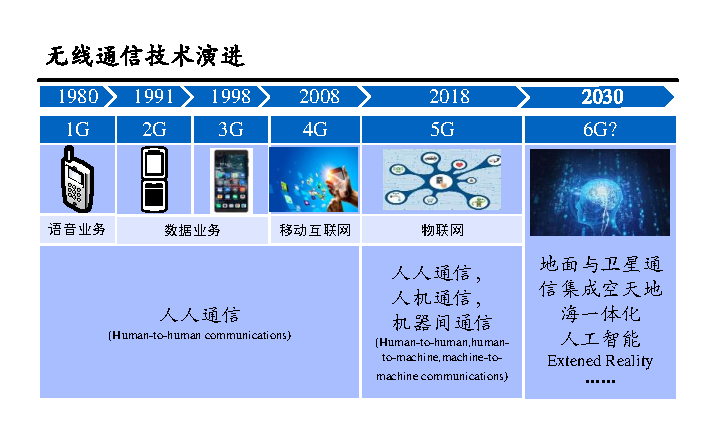
\includegraphics[width=16cm]{figures//chap1//无线通信技术演进.pdf}
\caption{无线通信技术演进。}
\label{无线通信技术演进}
\end{figure}
\supercite{陈进2020浅析中国城市智能交通系统产业化发展趋势}   \supercite{Integrationofelectric}

随着我国科学技术的快速发展,车联网的研发成为现代智能交通发展的重要途 \cite{陈进2020浅析中国城市智能交通系统产业化发展趋势}
通信行业产生的电力消耗巨大,预计到 2025 年,通信行业将消耗全球 20\%的电力 \cite{吕婷5G基站节能技术研究}
5G与LTEV2X将共同承载车联网业务    \cite{5G+MEC承载车联网业务传输性能测试与验证}
通信之道杨学志 \cite{杨学志2016通信之道}
\end{comment}
%{\CJKfamily{AR PL UKai CN}\color[RGB]{255,0,0}{红}}
\textcolor[RGB]{202,12,22}{}
随着科技的不断进步和社会的发展,现代车辆技术正经历着前所未有的变革 \supercite{SystematicSurvey10225497,DeepReinforcement9146378}。从传统燃油车到电动汽车,再到智能化驾驶系统,车辆技术的创新正在为我们的出行提供更加安全、高效、环保的选择。现代车辆技术不仅仅包括车辆的设计和制造,还涵盖了车辆动力系统、智能交通系统、车联网技术等多个方面。这些技术的综合应用使得车辆具备更高的性能、更低的排放、更智能的驾驶体验 \supercite{Autonomous9351818}。交通事故一直是社会的重要公共安全问题。通过引入智能化驾驶辅助系统和先进的驾驶辅助技术,车辆技术正在助力提高交通安全水平,减少交通事故的发生 \supercite{SecurityandPrivacy}。车辆越来越依赖于互联网和车联网技术。
道路车辆之间数据的的共享已成为一个重要的技术挑战,文献 \cite{刘雪娇186}中研究者在车联网数据共享与卸载进行了深入的研究 。
随着5G技术的逐渐商用,车联网将进入一个更加高速、低时延的通信时代。未来,6G技术的应用将为车联网提供更大的带宽和更先进的通信能力 \supercite{6GforVehicle}。更智能化的交通基础设施,包括智能交通信号灯、智能路牌等,将与车辆技术相互协作,提高整体交通效率。

2023年中国汽车出口量实现了显著的增长,首次在数量上超越日本,成为世界第一汽车出口国,实现了历史性的跨越。新能源汽车的上半场革命电气化正在如火如荼的进行的同时,下半场智能化已悄然拉开序幕,智能座舱与智能辅助驾驶为未来智能化汽车的发展奠定了基础。在商用车领域,萝卜快跑、美团外卖等平台使用自动驾驶实现更高效的工作效率与良好的用户体验。在乘用车领域,基于车道保持与自适应巡航控制(Adaptive Cruise Control, ACC)发展而来的智能辅助驾驶目前可以帮助驾驶员识别路面及周边信息,智能化的判断后进行转向变道刹车的动作 \supercite{SurveyofDeep8951131},智能座舱的发展不但兼顾了座椅电动调节影音娱乐等用户舒适化体验的需求,也可以更加高效的获取碰撞预警信息并进行行车环境感知数据共享等驾驶安全信息。由物联网发展而来的车联网将成为传统汽车向着智能化转型的强有力工具。

随着车联网技术的不断发展,车联网架构正朝着全方位立体化方向发展,常见的车联网架构包括车辆终端,车内的电子控制单元(Electronic Control Unit, ECU),车外的传感器,智能座舱等进行数据
的采集,任务的请求与接收,并提供高效的人机交互 \supercite{Edge10213996}。位于网络边缘的路边基站,边缘服务器,空中基站等由于处于网络边缘,距离车辆较近,因此可以在较低的
延迟下为车辆处理部分任务请求 \supercite{EdgeComputing2019,Autonomous9756370},但是受限于性能与磁盘空间,边缘设施往往难以帮助车辆完成大负荷任务
,位于远程的云服务器有着更高性能的集群服务器,也有更加完备的储存散热与灾备能力,可以为车辆提供边缘服务器难以处理的任务请求。
\begin{comment}
这里写一些车联网的架构,然后如图 \ref{车联网网络连接架构} 所示,
\begin{figure}[H]
\centering
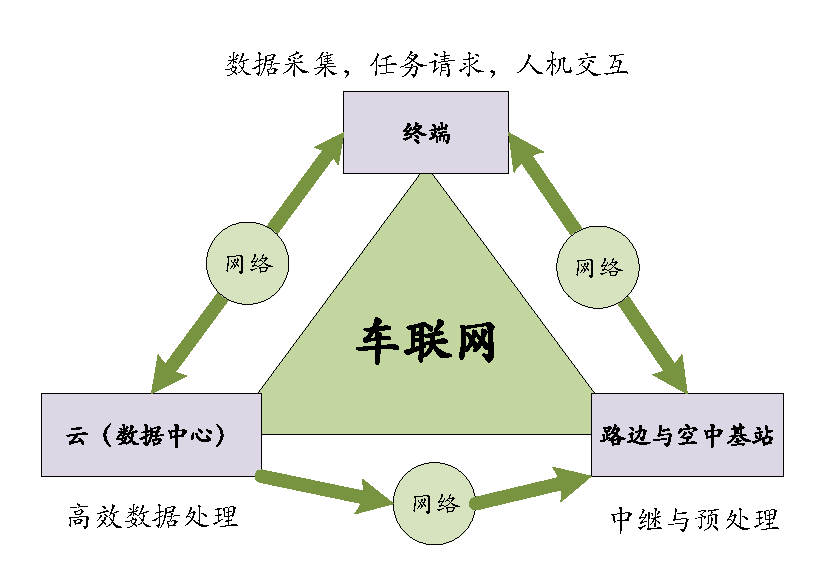
\includegraphics[width=12cm]{figures//chap1//车联网网络连接架构.pdf}
\caption{车联网网络连接架构。}
\label{车联网网络连接架构}
\end{figure}
\end{comment}


\section{国内外研究现状}\label{section1-2}
计算处理和信息交互过程 对高速行驶的车辆提出了计算密集和延迟敏感的要求。然而,车辆本身有限的计算和通信资源无法满足这些需求。
为解决这一问题,多路访问边缘计算(Multi-Access Edge Computing, MEC)技术已成为一种有前途的解决方案。最近,为了提高由云计算层和MEC层车辆网络架构组成的物联网边缘计算网络的有效性和鲁棒性,人们开展了一些研究。文献 \cite{Zhou2019}中,Zhou 等人提出了一种分层结构的车载网络计算框架,该框架由控制层、车载边缘计算服务器层和车载网络层组成。文献 \cite{Dai2022}中,Dai 等人研究了在MEC辅助服务架构中增强协同计算卸载服务,即多台MEC服务器与远程云协同实现计算密集型任务的卸载。一些研究提出了在云辅助移动边缘计算(Cloud-assisted mobile-edge computing, C-MEC)车载网络场景下提高计算卸载性能的方法。Tan和Hu 等人 \supercite{Tan2018}提出并解决了联合通信、缓存和计算问题,以优化车载网络的运行性能和成本效率,Wang 等人 将该问题表述为广义近地问题,并提出了一种博弈论算法来分析均衡问题 \supercite{Wang2020}。在文献 \cite{Wang2022}中, Wang 等人开发了一种分布式聚类机制,将车辆组织成多个合作的边缘服务器,以优化整个调度过程中的总收入。文献 \cite{Li2023}中,Li等人建立了车辆边缘服务缓存的分析模型,主要考虑了路侧单元(Road Side Unit, RSU) 之间的计算任务卸载和任务相互依赖。然而,上述方法只优化了功率控制和计算资源分配这两个指标中的一个。有些研究假定车辆保持恒定的发射功率,本文的方法采用了多方面的优化方法,包括优化车辆的发射功率和多车辆、多 MEC 服务器系统的计算资源分配。由于目标函数难以优化,因此带来了新的挑战。Nemirovski 和 Shapiro 提出了优化目标函数的凸近似方法 \supercite{Nemirovski2007}。 为了解决有两个变量的非凸问题,一些研究将原问题解耦为两个子问题,并采用块坐标下降方法(Block Coordinate Descent, BCD)来解决这两个子问题 \supercite{bertsekas1999nonlinear}。
\subsection{异构车联网络的鲁棒优化} \label{section1-2-1}
\begin{comment}
\begin{verbatim}
\end{comment}
高密度车载网络中,稀缺的频谱资源并不足以满足大量的车辆用户使用。为了应对未来道路上越来越多的车辆将接入车联网的需求,信道复用技术有望解决日益稀缺的通信频谱资源,可有效的提高频谱效率,但是,复用技术包括一对一复用,一对多复用以及多对多复用,大规模的使用信道复用技术会根据复用方式对相应的通信用户产生严重的干扰,在传统蜂窝网发展中,复杂通信的车联网干扰模型如图 \ref{复用技术下的通信干扰模型} 所示。该网络拓扑下车辆用户在某一载波信道上的干扰可以描述为:$\delta _{i}^{k}+\sum\limits_{j\ne i}{p_{j}^{k}g_{ij}^{k}}<I_{i}^{k}$,其中,$g_{ij}^{k}$为地面宏用户$j$在信道$k$上对车辆用户设备$i$的信道增益,$p_{j}^{k}$为宏用户$j$的信息发射功率,$\delta _{i}^{k}$为背景噪声,$I_{i}^{k}$为车辆用户$i$的在信道$k$上可正常通信时的最大可容忍的干扰阈值。在一些学术研究中,Zhou等人  \supercite{Zhou2017} 开发了一种5G频谱动态共享方法,并提出了专用短程通信(Dedicated Short-Range Communication, DSRC)和5G频谱的共享架构,以实现沉浸式体验驱动的车载通信。Tran等人  \supercite{Tran2019}  提出了一种综合方法来应对多服务器MEC辅助网络中任务卸载和资源分配的挑战。结果表明,当频谱资源稀缺时,有效的信道复用至关重要 \supercite{Liang2021}。 然而,这种方法通常会产生干扰,在车载通信场景中,信道复用造成的干扰往往会严重降低通信质量。为了处理中断概率约束,Xiao 等人 \supercite{Xiao2020} 假定信道状态信息(Channel State Information, CSI) 可以通过估计获得。Chen 等人 \supercite{Chen2022} 将中断约束条件转换为伯恩斯坦式不等式,以提出确定性优化问题。
\begin{figure}[H]
\centering
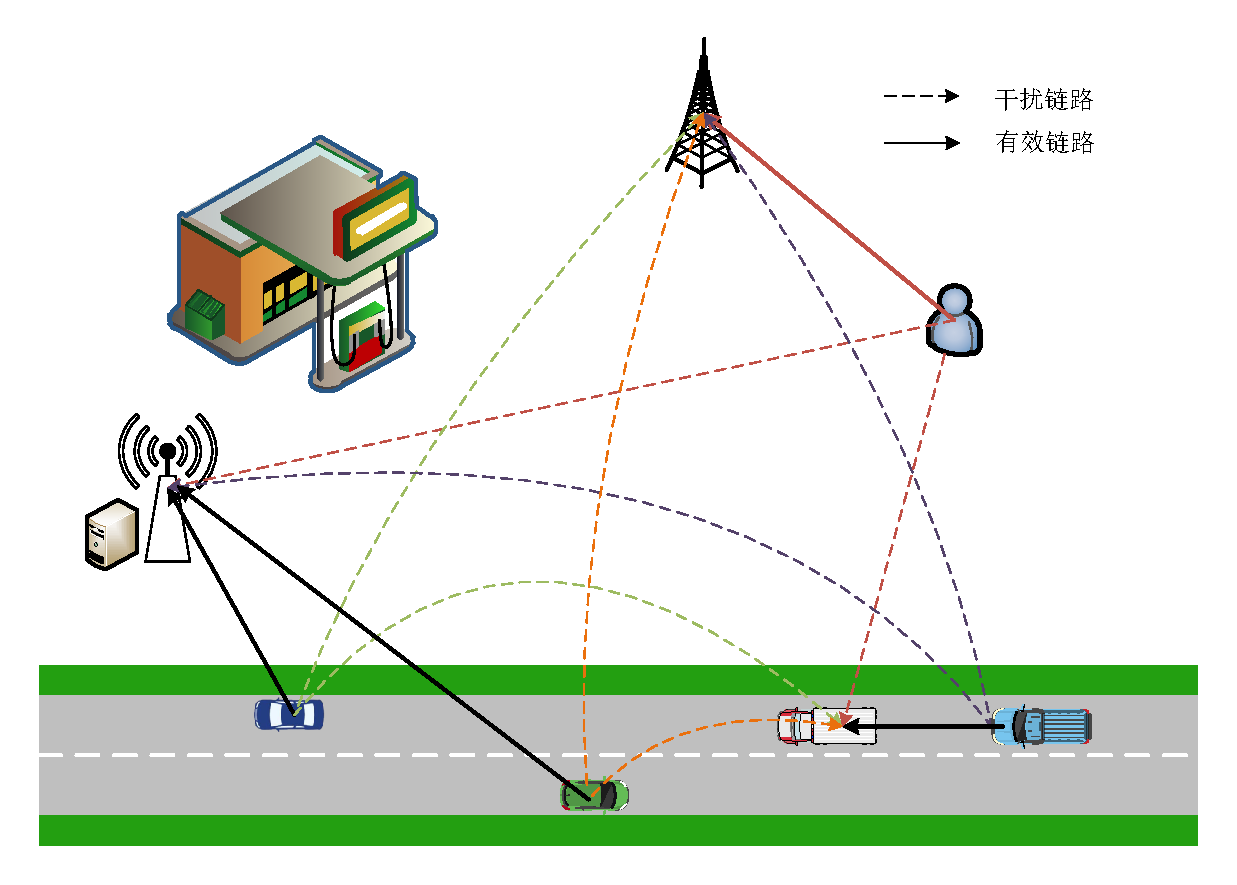
\includegraphics[width=10cm]{figures//chap1//车联网的干扰模型.pdf}
\caption{复用技术下的车联网通信干扰模型。}
\label{复用技术下的通信干扰模型}
\end{figure}
\subsection{云计算与边缘计算场景}\label{section1-2-2}
移动边缘计算MEC和移动云计算(Mobile Cloud Computing, MCC)是5G网络中崭露头角的两种新型架构,它们常应用于物联网设备的任务卸载过程中,特别在提供低延迟、高可靠性的计算服务方面发挥着关键作用。与低移动性的传统移动通信网络不同,当快速移动的车辆与不同的 MEC 服务器通信时,车辆高移动性下的多普勒效应给 C-MEC 通信带来了挑战。在具有动态特性的网络场景中,确定性信道状态信息已不足以描述信道状态。传输过程中产生的多普勒效应会严重影响 CSI 的小范围衰减,导致信道快速变化。换句话说,所使用的 CSI 已经过时。为了描述多普勒频移对信道的影响,可以使用一阶高斯$-$马尔科夫过程(First-order Gauss-Markov process)\supercite{CCO}。为了提高低通信延迟和计算延迟的性能,车载设备的延迟容忍度和传输可靠性都有所降低。因此,必须提出更高的要求。在文献 \cite{Li2020} 中 Li 等人为了确保车载通信链路的可靠性,引入了中断概率约束。当指数积分函数的精确表达式存在时,有必要考虑近似闭式表达式,使其具有可操作性,从而降低计算复杂度。

在C-MEC车载网络中,拥有频谱资源的授权车辆直接与RSU通信。然而,在高密度车载网络中,稀缺的频谱资源并不充足 \supercite{Xie2020}。Zhou等人 \supercite{Zhou2017} 开发了一种5G 频谱动态共享方法,并提出了DSRC和5G频谱的共享架构,以实现沉浸式体验驱动的车载通信。
%文献 \cite{Tran2019} 中,Tran等人提出了一种综合方法来应对多服务器MEC 辅助网络中任务卸载和资源分配的挑战。结果表明,当频谱资源稀缺时,有效的信道重用至关重要 \supercite{Liang2021}。然而,这种方法通常会产生干扰,在车载通信场景中,信道重用造成的干扰往往会严重降低通信质量。为了处理中断概率约束,Xiao 等人  \supercite{Xiao2020} 假定 CSI 可以通过估计获得。因此,将中断约束条件转化为伯恩斯坦式不等式,以提出确定性的优化问题 \supercite{Chen2022}。此外,由于不确定约束的特点,本文采用了伯恩斯坦方法。
总之,现有研究解决了云计算中的功率控制和计算资源分配问题,这有助于高动态环境下的车载网络中的 MEC。此外,也没有研究试图确保通信质量和延迟要求令人满意。
\subsection{无人机辅助车联网与轨迹优化}\label{section1-2-3}
近来,空地一体化作为提高无线通信质量最可行的解决方案之一,引起了业界和学术界的广泛关注。人们对空地一体化通信领域进行了广泛的关注和研究 \supercite{OUC,SDR}。由于具有部署灵活、远程操作和中继能力强等特点,空中无人机(Unmanned Aerial Vehicle, UAV)被选为地面网络的辅助设备 \supercite{ACO}。然而,当无人机加入异构场景时,空地一体化通信网络将面临两大挑战。首先,当采用信道复用模式提高频谱效率时,多用户干扰是一个棘手的问题。特别是在不确定的信道环境下,多用户干扰会极大地影响通信的有效性和鲁棒性,因此实现有效的干扰管理是一个重大挑战。其次,空地一体化异构车载网络(Air-Ground Heterogeneous Vehicular Network, AGHVN)是分层的,蜂窝用户(Cellular User Equipment, CUE)和车辆用户( Vehicular User Equipment, VUE)分别作为领导者和跟随者。然而,蜂窝用户和车辆用户是不同的利益相关者,他们为了各自的利益而竞争。平衡各方利益是一项挑战。因此,空地一体化异构车载网络的广泛部署仍面临紧迫挑战。

一些作者重点研究了空地一体化网络架构设计和资源管理 \supercite{OUC,OSI}。在异构蜂窝网络中,无人机被用来协助应急通信 \supercite{DSF}。在文献 \cite{SDR}中提出了一种为车辆用户动态分配频谱资源的控制框架,其中采用了 Lyapunov 优化理论。然而,尽管上述工作都重视提高 AGHVN 的性能,但将系统鲁棒性与资源分配相结合的研究却没有得到足够的重视。由于信道不确定性的存在,现有的资源分配策略很难实现鲁棒通信。因此,有必要考虑移动、遮挡、噪声等不确定因素对 AGHVN 鲁棒传输的影响。在边缘计算(MEC)架构辅助的车联网中,无人机是处理时间敏感任务的高效方法 \supercite{无人机辅助230770}。

\section{研究动机}\label{section1-3}
\begin{comment}
\textcolor[RGB]{202,12,22}{近年来,5G技术逐步商用化,无线通信技术的快速发展和应用为车联网通信的研究带来了巨大的机遇和挑战。5G移动技术可有效满足车联网的需求,为车联网的发展带来更好的解决方案。但与此同时,由于5G技术信道状态的复杂性以及车联网中移动用户的随机性使得诸多不确定因素共存于系统之中,如用户数量、信道状态、拓扑切换、可用信息以及用户信息安全等方面。可见这种高动态环境对于车联网无线可靠传输提出了新的挑战。}
\textcolor[RGB]{202,12,22}{
目前,专家学者主要困绕车联网中无线资源优化问题进行研究,通过结合5G通信技术与无线资源管理技术等来优化车联网络通信资源 \cite{RAI}。但是,并没有考虑在实际通信过程中车辆移动速度、通信环境的不确定性、以及不同信息在收发不平衡时会产生时延等情况。相比于传统的短期鲁棒优化,Lyapunov优化法是研究长期优化问题的有力方法论,它能够将长期约束转化为队列稳定性约束,并将长期目标函数转化为一系列短期子问题 \cite{ACAR}。此外,为了提升网络的稳定性和降低网络时延,传统的解决方法主要集中在物理层,通过物理层的功率控制来提升网络传输速率,稳定性,实现干扰管理等。然而,只考虑优化物理层传输速率,而忽略网络层的到达率,将导致到达率与传输数据之间的数据不平衡。数据的不平衡将导致数据积压和丢包,并最终导致网络延迟和不可靠性。因此,利用Lyapunov优化法来实现跨层资源鲁棒优化将成为5G车联网稳定高效通信的有效解决方法 \cite{Gao2020}。综上,如何基于Lyapunov优化法来满足多种用户QoS、快速收敛的分布式算法鲁棒优化算法具有实际意义。本文也将遵循这一技术路线分析算法的实现问题,针对车联网络通信场景 \cite{Song2022},在尽量减少信息交换量的前提下提出合适的迭代算法,降低5G车联网系统中节点的通信复杂程度,并实现多种性能指标的提升和折中。}
其中的参数“[width=$\backslash$textwidth]”指定图形的宽度0.6倍页宽。最后的效果如图 \ref{本文结构}所示。
\end{comment}
近年来,随着5G技术的逐步商用化,无线通信技术的迅猛发展和广泛应用为车联网通信的研究提供了前所未有的机遇,同时也伴随着诸多挑战。5G移动技术的出现,为车联网的发展提供了高效且可靠的解决方案。然而,由于5G技术信道状态的复杂性以及车联网中移动用户的随机性,系统内部存在众多不确定性因素,包括但不限于用户数量的变化、信道状态的波动、拓扑结构的频繁切换、可用信息的多样性以及用户信息安全等。这种高度动态的环境对车联网无线传输的可靠性提出了新的挑战,要求我们不断创新和优化相关技术以应对这些挑战。为了克服大规模车联网带来的挑战,一种与传统的分层博弈不同鲁棒的基于 Stackelberg 博弈的资源分配框架受到关注,斯塔克尔伯格博弈有望包括鲁棒的功率控制方案和价格机制,鲁棒的功率控制方案引入了概率约束来实现干扰管理。此外,指数积分法还将不确定形式转化为可解的封闭表达式。价格机制与功率控制方案相结合,在价格机制中,干扰被视为一种可分配给 VUE 的资源。通过对干扰收费,CUE 可以提高其效用。然而,当一个 VUE 想要通过提高传输功率来获得更高的速率时,就必须支付更多的干扰费。因此,价格机制可以限制 VUE 的自私行为,从而平衡各方利益。

云辅助移动边缘计算(C-MEC)为车载网络提供了丰富的计算资源,是一种前景广阔的任务卸载解决方案。本文提出了一种鲁棒的功率控制和任务卸载方案,以卸载计算任务并最大化 C-MEC 网络的效用。然而,不确定的信道状态会严重影响卸载任务传输的稳定性。此外,由于频谱资源有限,假设信道重用会导致复杂的同信道干扰。而且目标函数是一种非凸形式,很难求解。为了模拟信道的不确定性,考虑到车辆的移动性,采用了一阶马尔可夫过程。为了克服同信道干扰的限制,对信号链路实施了概率约束,以确保通信质量。采用伯恩斯坦近似法将原始约束条件转化为可解约束条件。在解决非凸鲁棒性优化问题时,严格采用了BCD方法和连续凸近似(Successive Convex Approximation, SCA)技术。为确定最优解,提出了一种鲁棒的功率控制和任务卸载调度算法。对提出的算法进行了数值模拟,以评估系统的性能。结果表明,与对比模型相比,该算法非常有效,尤其是在信道不确定的通信环境中。
\begin{comment}
\textcolor[RGB]{202,12,22}{根据国内外研究现状可知,对于 LTE-V2V 通信网络中的信道分配算法和功率分
配算法的研究已经取得了丰硕的成果。但上述文献对于资源分配算法研究时,信道
模型还不够多样化,不足以刻画真实的通信环境。在城市和高速公路上常见的大规
模车辆密集缓行的场景下,通信堵塞概率较高,各项通信性能急剧下降。为了解决
高密度车载网络场景下的干扰管理,本文在不确定信道环境下对 LTE-V2V通信网络
的干扰管理做出研究。
为了提高频谱资源,V2V 链路复用 CUE 信道是需要的。在不同复用规则下干
扰管理以及最优匹配的选择是重要的研究方向。本文分别对多个 V2V 车对复用一
个 CUE 信道,以及一个 V2V 车对复用一个 CUE 信道的提高频谱资源利用率的情
况进行研究。对于一对多复用情况同信道内用户数量多,干扰管理将是重点。而对
于一对一复用情况,最大化目标下匹配的选择机制是重点。在一对多复用情况下最
大化吞吐量这一优化目标是非凸的,对于一对一复用下最大化系统能效这一目标函
数也是非凸的,对于非凸目标函数的转化是需要解决的。本文针对车联网在不同优
化目标以及不同应用场景下的资源优化配置进行了研究。主要研究思路如下:首
先,针对不同通信环境场景下,根据优化问题构造出不同的优化目标函数以及为了
保证通信质量对鲁棒通信链路构造约束条件。其次,对于非凸目标函数进行凸优
化,将含有不确定性的鲁棒约束进行确定性转化,完成拉格朗日函数的构造。最
后,通过迭代算法求出最优解,仿真结果对算法可行性以及系统性能指标进行验
证。}

在5G车联网系统中,基站高密集部署大大提高了传输速率,然而节点之间频繁的通信也给整个系统的信息管理带来很大的挑战,由于动态通信环境的复杂性与时变性,往往对通信链路造成很大的干扰,导致通信系统中的参数具有不确定性。系统中参数的不确定性会严重影响用户的服务质量。不确定的信道可以有效地建模为一阶高斯-马尔可夫过程,该过程将当前信道实现描述为依赖于之前的信道实现,从而更接近于真实的信道。在V2I层通信网络中,普遍存在着数据的延迟以及较高误码率,而且通信链路受外界环境变化的影响非常大。因此,在系统建模时,必须考虑无线网络中存在的延迟问题。如何准确合理地对这些问题进行描述是解决这些问题的关键。此外,云端处理车辆的信息需要时间成本,将成本函数加入到网络总效用函数中可以以较小的时间成本获得最大的网络系统效用。
\end{comment}
%\begin{comment}

\textcolor[RGB]{202,12,22}{}
无人机,云边计算与车联网三者之间有着紧密的关系,无人机具有高机动性,能量受限,可以提供视距链路等特点,云计算与边缘计算具有高效率,高安全性,低时延等特点,而车联网的特点是大规模,高动态,高复杂性的拓扑结构,
%如图 \ref{5G通信与车联网融合挑战}所示,
这些因素都会影响车联网用户信息的可靠传输。由此,在含有多种信道不确定性因素的动态车联网络环境中,能够提供高速率、高可靠、低时延的移动通信是一个亟需解决的问题。
\begin{comment}
\begin{figure}[H]
\centering
\includegraphics[width=8cm]{figures//chap1//5G通信与车联网融合挑战.eps}
\caption{无人机辅助的车联网络任务卸载的融合挑战}
\label{5G通信与车联网融合挑战}
\end{figure}
%简单的说,\LaTeX 是一种对文字进行排版处理的程序语言,尽管它的功
\end{comment}
\section{论文结构安排}\label{section1-4}
本文以5G环境下的车联网为背景,在可视路径下充分体现了车辆用户的移动性,分别研究了无人机辅助静态车辆密集网络、动态环境下云计算边缘计算背景下车辆任务卸载、无人机辅助动态车辆任务卸载三个通信场景,在考虑了功率约束、无人机移动性约束、车辆用户服务质量约束等条件下,以吞吐量、系统能效为指标,对无人机轨迹、车辆功率控制、边缘服务器资源分配进行联合优化,通过博弈论、拉格朗日法、SCA法、交替优化法、贝恩斯坦近似法、积分变换法等方法提升车联网的高效性与可靠性。本文结构如下:

第2章主要研究了基于鲁棒博弈论的功率分配方案。构建了一个空地一体网络,无人机充当空中基站为地面的车辆用户提供任务卸载,车辆对无人机(Vehicle to Unmanned Aerial Vehicle, V2U)链路复用蜂窝宏用户的频谱资源,使用Stackelberg博弈来建模宏用户与车辆之间的关系,宏用户将其基站所能接受的最大干扰通过定价的方式出售给车辆用户,车辆用户根据其购买的干扰额度来决定自己的最佳发射功率,可以在最大可能的提高自己的通信服务质量的同时也让宏用户收获最大的收益。当车辆用户给基站造成的跨层干扰总量超出设定的干扰阈值时,基站会采取提高干扰定价的策略,以此来减少车辆用户购买的干扰份额。反之,如果干扰总量低于干扰阈值,基站则会降低干扰定价,鼓励车辆与无人机链路增加其购买的干扰份额。通过数值仿真,验证了这一算法的稳定性和实用性。

第 3 章主要研究了云计算与边缘计算协同的通信车辆的功率分配与计算卸载的方案,在本章中,充分考虑了车辆的高速移动性,使用小尺度衰落建模了非理性情况下车辆用户与路边边缘服务器之间的信道衰落模型,同时通过分簇的方式将每个V2R链路共享同样的频谱资源,并通过Bernstein 近似方法进行干扰管理,处理了复杂的干扰造成的非凸中断概率约束,SCA法近似了复杂难以求解的目标函数,最后通过Lagrange 法迭代更新了最优的车辆功率分
配与云服务器提供的最优的计算资源分配。仿真结果验证了算法的有效性并通过对比发现了车辆高速移动性带来的消极影响。

第 4 章主要研究无人机辅助的车辆用户任务卸载与轨迹规划方案,本章考虑了更加实际的物理场景,通过优化每个时隙的无人机飞行轨迹、车辆发射功率以及时隙资源分配来最大化系统的能量效率,并且考虑了双向车道的场景,无人机空中基站与地面基站同时帮助车辆进行任务卸载,随着逐渐驶离地面基站的车辆通信质量越来越差,无人机可以调整飞行姿态以靠近这部分车辆来提供任务卸载。然后通过积分变换将非凸的中断概率约束转化成简单可解的形式,通过泰勒展开将难以求解的无人机轨迹问题展开成凸问题。最后仿真结果验证了算法的有效性并通过对比展示了无人机轨迹规划方案效果优于其他两种方案。


\begin{comment}
本文的整体结构流程如图 \ref{结构安排}所示。    占用的正交信道
\begin{figure}[H]
\centering
\includegraphics[width=16cm]{figures//chap1//总体结构安排2.eps}
\caption{研究内容的总体结构安排。}
\label{结构安排}
\end{figure}
\end{comment}
\begin{comment}


本文采用的技术路线是考虑V2I通信链路中的移动边缘计算、中断概率以及信道增益不确定性的实际应用背景,根据通信系统中参数不确定性的特点,采用最优化理论与通信技术相结合的研究方法。本项目在理论分析的基础上,以数值仿真方法进行验证,开展V21通信链路研究。综上所述,本项目拟采用的技术路线如下图 \ref{技术路线图}所示:
\begin{figure}[H]
\centering
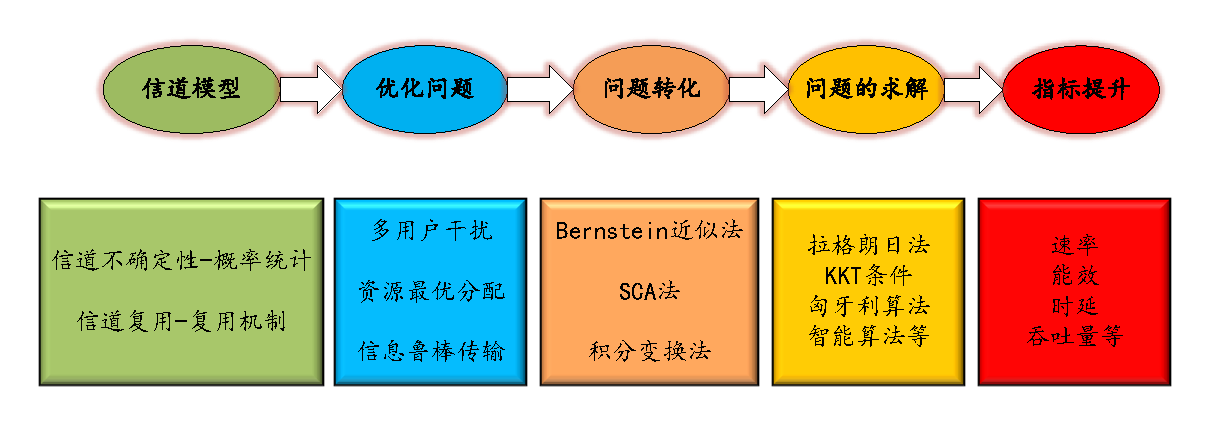
\includegraphics[width=16cm]{figures//chap1//技术路线图.pdf}
\caption{技术路线图。}
\label{技术路线图}
\end{figure}
\end{comment}

\begin{comment}


\textcolor[RGB]{202,12,22}{
在处理长期优化问题时,李雅普诺夫优化是目前应用广泛的一种有力方法论,它能够将长期约束转化为队列稳定性约束。通过Lyapunov优化法,包括构造联合向量、Lyapunov 漂移函数,Lyapunov漂移惩罚函数,可以将长期的优化目标(目标函数和约束条件)转化为队列稳定性条件,最终拆分为一系列短期子问题。在满足不同用户的服务质量要求和业务队列稳定性条件下,基于Lyapunov优化法所提出的跨层资源策略可以揭示吞吐量和传输时延等性能指标之间的权衡关系。经过上述非凸问题的转化过程,我们可以得到由闭式表达式组成的确定性鲁棒优化问题,再利用传统的求解方式,如:穷举法,KKT条件,构造拉格朗日函数法,匈牙利算法等,便可以获得转化后优化问题的最优解。整体的技术路线图如图\ref{技术路线图}所示。}


\begin{verbatim}
以下是解决pdf文件复制乱码问题(方便论文查重,我已经按照第一种办法做了,如果有个别同学还是不成功,请按照后边方法,照做一下)!!!下面是另外两种办法,共三种办法!!!
(1) 在YSUthesis.cls的Line142,加上``\setCJKmainfont{新宋体}第一种办法!''
%%上面一行是解决pdf文件复制乱码问题!!!下面是另外两种办法,共三种办法!

(2) 在template.tex文件的\begin{document}前边,加上
``\usepackage{ccmap}删掉前边的注释!为了解决论文查重,PDF文件复制出现乱码问题,请去掉这行前面的注释,编译完成后,使用Adobe Acrobat 删掉论文前面多余的两页即可!!!不知道是什么原因,但是这样可以解决问题,有待大家找到更好的解决办法!!!这种方法在编译过程中会终止,需要回车一下!!!''

(3) 在template.tex文件的\classification{O226}前边,加上
``为了解决论文查重,PDF文件复制出现乱码问题,请去掉这行前面的注释,编译完成后,使用Adobe Acrobat 删掉论文前面多余的两页即可!!!不知道是什么原因,但是这样可以解决问题,有待大家找到更好的解决办法!!!''
\end{verbatim}
\end{comment}


%注意!第一章不要有``本章小结"!!!

%!Mode:: "TeX:UTF-8"
%\chapter{车联网技术的网络资源优化理论基础}
%\chapter{基于博弈论的鲁棒干扰管理异构车载网络中的大规模空地一体化通信异构车载网络}  基于博弈论的
\chapter{基于博弈论的无人机辅助异构车联网络的鲁棒功率控制}
\begin{comment}
\label{chap:figures}
插图主要涉及到:单个居中图形;两个并排图形;两个以上的并排或者堆叠的图形;图题;图形的引用;
\end{comment}
\section{引言}\label{section2-1}
作为智能交通系统(Intelligent Traffic Systems, ITS)最有前途的解决方案,车联网(Internet of Vehicles, IoV)有望满足快速增长的需求,如交通效率、
驾驶体验和事故处理。然而,由于车辆密度和用户需求的快速增加,单小区网络的频谱效率变得较低 \supercite{TFL}。因此,异构车联网络的部署已成为一种趋势 \cite{ACAR}。

近年来,空地一体化作为提高无线通信质量的最可行的解决方案之一,引起了工业界和学术界的广泛关注。由于无人机具有部署灵活、远程操作和中继能力,选择空中无人机来辅助地面网络可提升网络效率 \supercite{ACO}。然而,当无人机加入异构场景时,空地综合通信网络将
面临两大挑战。首先,当使用信道复用模式来提高频谱效率时,多用户干扰是一个棘手的问题。有效和鲁棒的通信在很大程度上受到多用户干扰的影响,特别是在不确定的信道环境中,因此实现有效的干扰管理是一个重大挑战\supercite{CCO}。 其次,空地集异构车辆网络(AGHVN)是分层的,其中蜂窝用户CUE和车辆用户VUE分别充当领导者和追随者。然而,CUE和VUE是不同的利益相关者,他们为自己的利益而竞争,平衡各方利益是一项挑战,使用博弈论的决策方法可以有效的构建CUE和VUE之间复杂利
益关系 \supercite{胡益恺智能车辆决策方法研究综述}。因此,空地一体化异构车载网络的广泛部署仍然带来紧迫的挑战。
\begin{comment}
\subsection{NOMA技术的理论基础}\label{section2-1-1}
大多数情况下,需要插入的图形是单个的时候可以使用如下环境:

\subsection{CR技术的理论基础}\label{section2-1-2}
其中的参数“[width=$\backslash$textwidth]”指定图形的宽度0.6倍页宽。最后的效果如图\ref{ysulogo}所示。
\begin{figure}[hptb!]
 \centering\small
 
\includegraphics[width=0.6\textwidth]{ysulogo}
 \Figcaption{单个居中图形}\label{ysulogo}
\end{figure}
\subsection{MEC技术的理论基础}\label{section2-1-3}

最终结果如图\ref{fig-dbfig}所示。
\begin{figure}[hptb!]
  \centering\small
  \begin{minipage}[t]{0.5\linewidth}
    \centering
    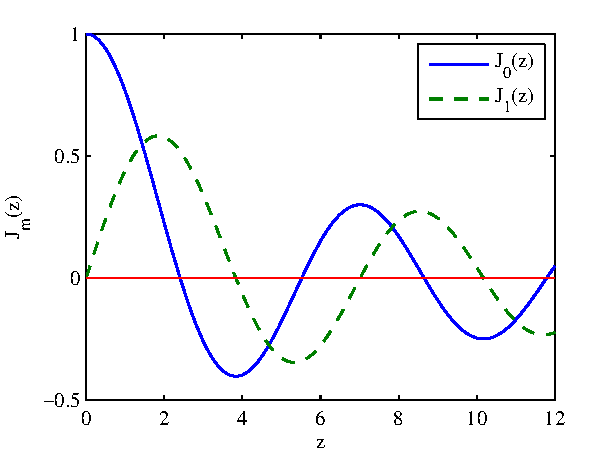
\includegraphics[width=\textwidth]{chp-2_bessel_j}
    (a) 子图a图题子图a图题子图a图题
  \end{minipage}%
  \begin{minipage}[t]{0.5\textwidth}
    \centering
    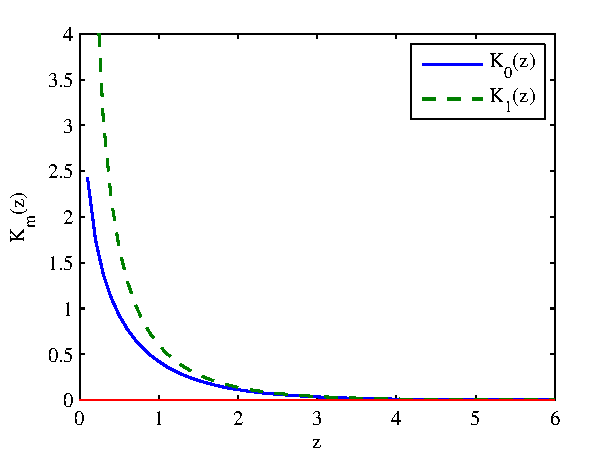
\includegraphics[width=\textwidth]{chp-2_bessel_k}
    (b) 子图b图题子图b图题子图b图题
  \end{minipage}
    \Figcaption{两个并排图形}\label{fig-dbfig}
 \end{figure}
\end{comment}
\section{系统模型与问题描述}\label{section2-2}
\subsection{系统及信道模型}\label{section2-2-1}
本章考虑了一种上行链路空地一体化通信场景,在这种场景中,众多车对无人机(V2U)小区覆盖在一个宏蜂窝之下。
如图 \ref{天地网络系统模型} 所示,无人机固定悬停并部署在交通拥堵路段,负责接收其覆盖范围内车辆的信号并
将其发送到基站(Base Station, BS)。值得注意的是,所有无人机都是双工的,配备有接收天线和发射天线,因此接收和发射过程
可以同时完成。通信中的CUE和VUE集合分别索引为$\mathcal{S}_0= \{0\}$ 和$\mathcal{S}_l=\{1, 2,..., N\}$。
为了提高频谱利用率,实现多用户联合通信,V2U 通信重复使用了CUE 的上行信道。但是会产生严重的多用户干扰,
限制了信号链路的通信。如图 \ref{天地网络系统模型} 所示,信号链路(蜂窝链路和同信道 V2U 链路)和干扰链路(CUE-V 链路、V-BS 链
路和 V2U 干扰链路)被区分开来。

假设无人飞行器的飞行高度为 $H_n$,则 VUE$_{k}$ 与 UAV$_{n}$ 之间的距离为:
\begin{eqnarray}\label{E2-1}
h_{k,n}=\sqrt{H_n^2+(\|W_k-W_n\|)^2},           &k, n\in \mathcal{S}_l
\end{eqnarray}
其中 $W_k$ 和 $W_n$ 是 VUE$_{k}$ 与 UAV$_{n}$的位置信息,  CUE 与BS之间的距离为:
\begin{eqnarray}\label{E2-2}
h_{0,0}=\sqrt{H_0^2+(\|W_0-W_{BS}\|)^2}
\end{eqnarray}
其中,$W_0$ 和 $W_{BS}$ 为 CUE 和 BS 的位置,$H_0$ 为 BS 上信号接收器的垂直高度。VUE$_{k}$ 与 BS 之间的距离为 $h_{k,0}$,CUE 与 UAV$_{n}$ 之间的距离为 $h_{0,n}$,$h_{k,0}$和$h_{0,n}$的表达式类似于 \eqref{E2-1}和 \eqref{E2-2}。

\begin{figure}[H]
\centering
\includegraphics[width=10cm]{figures//chap2//第二章系统模型.eps}
\caption{空地网络系统模型}
\label{天地网络系统模型}
\end{figure}
\begin{comment}
\begin{figure}[hptb!]
 \centering\small
 \includegraphics[width=0.6\textwidth]{figures//chap2//cchina1.pdf}
 \Figcaption{无人机的系统模型}\label{sysjktemuav}
\end{figure}
\end{comment}

蜂窝链路和同信道 V2U 链路的大规模衰落可分别表示为:
\begin{eqnarray}\label{E2-3}
g_{0,0}=L_{0,0}h_{0,0}^{-\alpha}
\end{eqnarray}
\begin{eqnarray}\label{E2-4}
g_{n,n}=L_{k,n}h_{k,n}^{-\alpha},          &k, n\in \mathcal{S}_l, k=n
\end{eqnarray}
其中,$L_{0,0}$ 和 $L_{n,n}$ 是蜂窝链路和同信道 V2U 链路的阴影衰减效应。$\alpha$ 是路径损耗指数。虽然车辆与无人机之间的传输链路可视为借助无人机在道路上空进行的 LoS 通信,
但仍存在一些影响信道增益的因素,如通信终端的相对移动、信道估计误差以及不可避免的信道不确定性。因此,小尺度衰落不容忽视。根据文献 \cite{CCO},它遵循截断指数分布。为了描述信
道增益的不确定性,引入了一个参数 $G$,$G$ 是一个独立的同分布随机变量,其概率密度函数为 $f_G (x)=e^{-x}$ 。信号链路 $n$ 的实时信干噪比(Signal to Interference plus Noise Ratio ,SINR)可表示为:
\begin{eqnarray}\label{E2-5}
\gamma_{n}(p_n)=\frac{p_{n}G g_{n,n}}{I_n}, k\in\mathcal{N},n\in\mathcal{N}
\end{eqnarray}
其中,$g_{n,n}$ 是给定时隙内的估计增益。同信道 V2U 链路 $n$ 的干扰可视为测量值,其表达式为:
\begin{eqnarray}\label{E2-6}
I_n=p_0 g_{0,n}+\!\!\!\sum\limits_{k=1,k\neq n}^N\!\!\!\! p_k g_{k,n}+\delta^2, \quad k\in\mathcal{N},n\in\mathcal{N}
\end{eqnarray}
其中,$p_k$ 表示第 $k$ 个 VUE 的传输功率。$p_0$ 是 CUE 的传输功率。$\delta^2$ 是噪声干扰。

为处理不确定参数 $G$,确保 V2U 通信质量,引入了以下中断概率约束,
\begin{eqnarray}\label{E2-7}
\textrm{Pr}\left\{\gamma_{n} \leq \gamma_{th}\right\}\geq1-\varepsilon,\quad  n\in\mathcal{S}_l
\end{eqnarray}
其中,$\textrm{Pr}\{\cdot\}$为概率约束,$\gamma_{n}$ 表示第 $n$ 个同频 V2U 链路的瞬时 SINR。$\gamma_{th}$是给定的目标 SINR阈值,。$\varepsilon$ 是中断概率阈值,$\varepsilon \in (0,1)$ 。

为了考虑不确定的信道增益,并使用遍历容量来显示网络性能,
\begin{eqnarray}\label{E2-8}
R_{er}=\int_{0}^{\infty} W \log(1+\gamma_{n})\Pr(\gamma_{n})\, d(\gamma_{n})
\end{eqnarray}
其中,$W$ 是复用信道的带宽,$\Pr(\gamma_{n})$ 是 $\gamma_{n}$ 的概率分布函数。
根据詹森不等式可知,
\begin{comment}

\begin{eqnarray}\label{E2-9}
 \begin{array}{lll}
&\!\!\!\!\!\!\mathbb{E}\{W \log(1+\gamma_{n}\}=\int_{0}^{\infty} W \log(1+\gamma_{n})\ \Pr(\gamma_{n})\, d(\gamma_{n})\\
&\quad\quad\quad\quad\quad\quad\quad\!\!<W\log(1+\mathbb{E}\{\gamma_{n}\})\\
&\quad\quad\quad\quad\quad\quad\quad\!\!=W\log(1+\bar{\gamma}_{n})
 \end{array}
\end{eqnarray}

\end{comment}
\begin{align} \label{E2-9}
\mathbb{E}{W \log(1+\gamma_{n})} &= \int_{0}^{\infty} W \log(1+\gamma_{n})\ \Pr(\gamma_{n}), d(\gamma_{n}) \\
&< W\log(1+\mathbb{E}{\gamma_{n}})   \notag \\
&= W\log(1+\bar{\gamma}_{n})                \notag
\end{align}
其中 $\bar{\gamma}_{n}\!=\mathbb{E}\{\!\frac{p_{n}G g_{n,n}}{I_n}\}
\!=\!\frac{p_{n}g_{n,n}}{I_n}$ ,是香农容量是遍历容量的上限,通过信道编码技术可以使遍历容量接近上限。
因此,根据香农定理计算出的 VUE 的确定性等效传输速率为:
\begin{eqnarray}\label{E2-10}
R_{n}=W\log(1+\bar{\gamma}_{n}(p_n)),\quad  n\in\mathcal{N}
\end{eqnarray}
\subsection{博弈论问题的描述}\label{section2-2-2}
在空地一体化异构的车载网络(AGHVN)中,频谱所有者 CUE 可以对干扰进行定价,并将 VUE 的收费作为其利润。在 V2U 小区中,VUE 的效用是传输速率与购买干扰成本之间的差额。
考虑到 CUE 和 VUE 都是自私自利的,它们都愿意为自己的利益而竞争。因此,数学框架符合 Stackelberg 博弈模型,其中 CUE 和 VUE 分别是领导者和追随者。此外,还考虑了
 CUE 的通信约束。第$n_{th}$ 个V2U 单元的下子博弈可表述为:
\begin{comment}
\begin{eqnarray}\label{11}
\end{comment}
\begin{align} \label{E2-11}
&P_1: \max\limits_{p_{n}} U_{n}=R_{n}\!\!-c_{n} p_n g_{n,0}                                                          \\
&\text { s.t. }
\quad \!\!\!\!\! \textrm{Pr}\left\{\gamma_{n}(p_n) \geq \gamma_{th}\right\}\geq1-\varepsilon  \tag{\ref{E2-11}{-1}}  \label{E2-11-1}\\
& \quad \quad \quad \!\!\!\!\! 0\leq p_n\leq p_{n,\textrm{max}}                               \tag{\ref{E2-11}{-2}}  \label{E2-11-2}
\end{align}
其中,$U_{n}$ 是第 $n$ 个 V2U 信号链路的效用,$p_{n,\textrm{max}}$ 是车辆发射功率的上限。

作为领导者,价格策略应保证每个用户都有正收益。因此,蜂窝网络的上子博弈可以表述为:
\begin{align} \label{E2-12}
&P_2: \max\limits_{\mathbf{c}} U_0=\sum\limits_{n=1}^N c_{n} p_n(c_{n}) g_{n,0}                    \\
& \text { s.t. }
\quad \!\!\!\!\! R_{n}\{p_n(c_{n})\} \geq c_{n} p_n(c_{n}) g_{n,0}          \tag{\ref{E2-12}{-1}}  \label{E2-12-1}\\  %信噪比中断概率约束
& \quad \quad \quad \!\!\!\!\! 0\leq c_n\leq c_{n,\textrm{max}}             \tag{\ref{E2-12}{-2}}  \label{E2-12-2}  %功率阈值
\end{align}
其中,$U_{0}$ 是蜂窝链接的效用,$c_{n,\textrm{max}}$ 是价格上限。

此外,通过寻找子博弈的纳什均衡(Nash Equilibrium, NE),可以得到所提出的斯塔克尔伯格博弈的博弈均衡(Game Equilibrium, GE)。关于NE和GE在文献 \cite{RAI}中有如下的详细描述:

设 $c_i^*$ 是上层子博弈优化问题 \eqref{E2-12} 的解,$p_i^*$ 是下层子博弈优化问题 \eqref{E2-11} 的解。那么,对于任意 $(c_i,p_i)$,如果满足以下条件,点 $(c_i^*,p_i^*)$就是所提议的斯台克尔伯格博弈的 GE:
\begin{equation} \label{E2-13}
U_0\left(c_i^*, \mathbf{c}_{-i}^*, \mathbf{p}_i^*\right) \geq U_0\left(c_i, \mathbf{c}_{-i}^*, \mathbf{p}_i^*\right), \quad i \geq 1, i \in \mathcal{I}
\end{equation}
\begin{equation} \label{E2-14}
U_{\text {sum }}\left(p_i^*, \mathbf{p}_{-i}^*, \mathbf{c}_i^*\right) \geq U_{\text {sum }}\left(p_i, \mathbf{p}_{-i}^*, \mathbf{c}_i^*\right) \quad i \geq 1, i \in \mathcal{I}
\end{equation}
%一般来说,可以通过确定子博弈的完美纳什均衡(NE)来获得 Stackelberg 博弈的通用均衡。在 Stackelberg 博弈中,车辆用户和宏用户以非合作博弈竞争。下层网络中的每个用户都希望通过调整其功率策略来实现效用总和的最大化。对于非合作博弈,NE 被定义为没有一方能提高其效用的可行点。在此点上,任何一方都无法通过单方面改变策略来提高其效用。  调整一下这句话使其更加通顺

一般而言,为了获取Stackelberg博弈的通用均衡,首先需要确定其子博弈的完美纳什均衡。在Stackelberg
博弈框架下,车辆用户和宏用户进行非合作博弈,竞争各自的利益。在下层网络中,每个用户均致力于通过优化其功率策
略,实现效用总和的最大化。对于非合作博弈而言,纳什均衡(NE)是一个至关重要的概念,它代表了一种策略组合,在
该组合下,没有任何一方能够通过单方面改变其策略来获得更高的效用。

%因此,GE 的计算过程如下 :在领导者与追随者的博弈中,领导者宣布非统一价格 领导者$-$追随者博弈中宣布非统一价格,首先计算第 $i$ 个追随者的最佳响应 $p_i$。然后,领导者观察并调整干扰定价策略 $c_i$,其目的是最大化上层网络的总效用。根据上层网络的总效用最大化结果,跟随者也可预见调整后的价格策略,并反复执行上述过程,直到最优价格策略 $c_i^*$ 和最优 功率策略$p_i^*$ 得出。
因此,通用均衡(GE)的计算过程如下:在领导者与追随者构成的Stackelberg博弈中,领导者首先宣布非统一价格策略。随后,
计算第$i$ 个追随者在给定领导者价格策略下的最佳响应$p_i$,接着,领导者根据观察到的追随者响应,调整其干扰定价策略$c_i$,
旨在最大化上层网络的总效用。基于上层网络总效用的最大化结果,追随者能够预见领导者调整后的价格策略,并据此
调整自身的功率策略。这一过程反复进行,直至达到最优价格策略$c_i^*$和最优功率策略$p_i^*$
,从而确保Stackelberg博弈达到均衡状态。
\section{博弈问题求解}\label{section2-3}
\subsection{概率约束的转化}\label{section2-3-1}
从 \eqref{E2-6}和 \eqref{E2-7}可以看出,中断概率约束可以表示为:
\begin{equation}\label{E2-15}
\textrm{Pr}\left\{\frac{p_{n}G g_{n,n}}{I_n} \geq \gamma_{th}\right\}\geq1-\varepsilon
\end{equation}
由于 $G$ 的概率密度函数为 $f_G (x)=e^{-x}$,因此可通过变量积分得到:
\begin{equation}\label{E2-16}
\int_{0}^{\frac{\gamma_{th}I_{n}}{p_n g_{n,n}}} e^{-x}\, dx\leq\varepsilon
\end{equation}
%可以认为:
\begin{equation}\label{E2-17}
\frac{p_n g_{ n,n}}{I_{n}}\geq\frac{-\gamma_{th}}{\ln(1-\varepsilon)}
\end{equation}

因此,中断概率约束的确定性表达式可求得如下:
\begin{equation}\label{E2-18}
\frac{-\gamma_{th} I_{n}}{\ln(1-\varepsilon)}-p_n g_{n,n}\leq0,\quad\forall n\in\mathcal{N}
\end{equation}
\subsection{求解下层子问题}\label{section2-3-2}
通过转换概率约束条件,可以得到一个资源分配的确定性优化问题。
\begin{align}  \label{E2-19}
&P_3: \max \limits_{p_{n}} R_{n}\!\!-c_{n} p_n g_{n,0}              \\
&\text { s.t. }
 \quad \!\!\!\!\! \frac{-\gamma_{th} I_{n}}{\ln(1-\varepsilon)}-p_n g_{n,n}\leq0 \tag{\ref{E2-19}{-1}} \label{E2-19-1}\\ %信噪比中断概率约束
& \quad \quad \quad \!\!\!\!\! 0\leq p_n\leq p_{n,\textrm{max}}                  \tag{\ref{E2-19}{-2}} \label{E2-19-2}  %功率阈值
\end{align}

由于 $P_3$ 是一个标准的凸优化问题,因此可以构造拉格朗日函数来求解最优解。 式 \eqref{E2-19} 的拉格朗日函数表述为:
\begin{eqnarray}\label{E2-20}
\begin{array}{lll}
\textit{L}_n(p_n, \lambda_n)=R_{n}\!\!-\!\!c_{n} p_n g_{n,0}\!\!-\!\!\lambda_n \left(\frac{-\gamma_{th} I_{n}}{\ln(1-\varepsilon)}-p_n g_{n,n}\right)
\end{array}
\end{eqnarray}
其中,$\lambda_n$ 是拉格朗日乘数,$\lambda_n \geq 0$。

使用次梯度法,可以得到拉格朗日乘数的迭代更新表达式,
\begin{equation}\label{E2-21}
\begin{array}{lll}
     \lambda_n^{(t+1)}=[\lambda_n^{(t)}\!\!+\!K_{\lambda}^{(t)}(\frac{-\gamma_{th} I_{n}^{(t)}}{\ln(1-\varepsilon)}-p_n^{(t)} g_{n,n})]^+
\end{array}
\end{equation}

其中 $I_{n}^{(t)}=$$p_0 g_{0,n}+\sum_{k=1,k\neq n}^N p_k^{(t)} g_{k,n}$。
$P_3$ 的卡鲁什$-$库恩$-$塔克(Karush-Kuhn-Tucker, KKT)条件为,
\begin{equation}\label{E2-22}
\begin{array}{rl}
\left\{
\begin{array}{lll}
     \frac{\partial \textit{L}_n(p_n, \lambda_n)}{\partial p_n}\!=\!\frac{W g_{n,n}}{p_n g_{n,n}+I_n}\!-\!c_n g_{n,0}\!-\!\lambda_n g_{n,n}\!=\!0\\
     \lambda_n \big(\frac{-\gamma_{th} I_{n}}{\ln(1-\varepsilon)}-p_n g_{n,n}\big)=0\\
     \lambda_n \geq 0
\end{array}
\right.
\end{array}
\end{equation}

每个 VUE 的最优传输功率为,
\begin{equation}\label{E2-23}
\begin{array}{*{21}{ll}}
 p_n^{*}=\frac{W}{c_n g_{n,0}-\lambda_n^{*}g_{n,n}}-\frac{I_n^{*}}{g_{n,n}}
\end{array}
\end{equation}

此外,迭代表达式如下,
\begin{eqnarray}\label{E2-24}
\begin{array}{lll}
\qquad p_n^{(t+1)}=\frac{W}{c_n g_{n,0}-\lambda_n^{(t+1)}g_{n,n}}-\frac{I_n^{(t+1)}}{g_{n,n}}
\end{array}
\end{eqnarray}

要证明 \eqref{E2-23}是 GE,就要讨论 NE 的存在性和唯一性。

存在性: 类似于文献 \cite{GT} 的描述,在 Stackelberg子博弈 \eqref{E2-12}中存在一个NE,其条件为:

1) $\mathbf{P}$ 是某个欧几里得空间 $\mathcal{R}^N$ 的非空凸紧凑子集,

2) $U_{\textrm{n}}(p_n)$ 在 $\mathbf{P}$ 中是连续的,在 $p_n$ 中是凹的。

\begin{proof}

1) 功率策略空间为 $\mathbf{P}=\{p_n:0\leq p_n \leq p_{n,\textrm{max}}\}$, 它是欧几里德空间 $\mathcal{R}^N$ 的一个非空、凸和紧凑子集。
2) 得到效用关于 $p_n$ 的一阶导数、
\begin{equation}\label{25}
\frac{\partial U_{n}}{\partial p_n}=\frac{Wg_{n,n}}{p_n g_{n,n}+I_n}-c_ng_{n,0}
\end{equation}
得到关于 $p_n$ 的二阶导数、
\begin{equation}\label{26}
\frac{\partial^2 U_{n}}{\partial p_n^2}=-\frac{W(g_{n,n})^2}{\big(p_n g_{n,n} +I_n\big)^2}<0
\end{equation}
由于 $U_{\textrm{n}}(p_n)$ 相对于 $p_n$ 的二阶导数总是小于 0,所以 $U_{\textrm{n}}(p_n)$ 在 $p_n$ 中是凹的。因此,在 Stackelberg子博弈 \ref{E2-12}中存在一个NE 。
\end{proof}\par

唯一性: 当$g_{n,n}$$>$$\sum\limits_{k=0,k\neq n}^N g_{k,n}$时,在所提的 Stackelberg子博弈中,NE是唯一的。

\begin{proof}
令 $p_{-n}(t)=[p_k(t)]_{k\in\mathcal{K},k\neq n}$,则
\begin{equation} \label{E2-27}
G_{-n}p_{-n}(t)=\sum\limits_{k=1,k\neq n}^N g_{k,n}p_k(t)
\end{equation}
其中 $G_{-n}=[g_{k,n}]_{k\in\mathcal{N},k\neq n}^T$ ,定义 $\Delta p_{n}(t)=p_{n}(t)-p_{n}^*$ ,可以得到:%\par
\begin{eqnarray}\label{E2-28}
\hspace{-0.2cm}
 \begin{array}{lll}
&\!\!\!\!\!\!\!|\Delta p_{n}(t+1)|=|p_{n}(t+1)-p_{n}^*|\\
&\quad \quad \quad \quad =\Big|\frac{\sum_{k=0,k\neq n}^N g_{k,n}(p_k^{(t)}-p_k^*)}{g_{n,n}}\Big|\\
&\quad \quad \quad \quad =\Big\|\frac{\sum_{k=0,k\neq n}^Ng_{k,n}}{g_{n,n}}\Big\|_\infty \big\|\sum_{k=0,k\neq n}^N\Delta p_{k}(t)\big\|_\infty
\end{array}
\end{eqnarray}

一般情况下,V2U 信号链路的信道增益大于干扰链路,所以 $g_{n,n}$$>$$\sum_{k=0,k\neq n}^N g_{k,n}$ 是可行的。然后,可以得到 $\|\frac{G_{-n}}{g_{n,n}}\|$$<$$1$ 。
$\big\|\sum_{k=0,k\neq n}^N\Delta p_{k}(t)\big\|_\infty=\max [\Delta p_{k}(t)]_{k\in\mathcal{N},k\neq n}$。因此,    %根据$l_\infty-$norm的定义,可以得出
$\delta p_{n}(t+1)$ 在迭代一段时间后可以趋近于零,而 $p_{n}(t+1)$ 可以趋近于唯一的最优点 $p_{n}^*$。因此,在 Stackelberg 子博弈中,NE 是唯一的。
\end{proof}
\subsection{求解上层子问题}\label{section2-3-3}
由\ref{section2-3-2}得到的VUE 的最优传输功率 $p_n$可用来求解上层子问题。
在上层网络中,根据 VUE 的最优传输功率 $p_n$,原来的上层子博弈可以重写为,
\begin{align}  \label{E2-29}
& \!\!\!\!\!\!\!P_4:\max\limits_{\mathbf{c}} \quad \sum\limits_{n=1}^N c_{n} p_n(c_{n}) g_{n,0}                    \\
\text { s.t. }
& W\log(1+\frac{p_{n}(c_{n}) g_{n,n}}{I_n}) \geq c_{n} p_n(c_{n}) g_{n,0}         \tag{\ref{E2-29}{-1}} \label{E2-29-1}\\  %信噪比中断概率约束
& p_n(c_{n})\!\!=\!\!\frac{W}{c_n g_{n,0}-\lambda_n g_{n,n}}-\frac{I_n}{g_{n,n}}  \tag{\ref{E2-29}{-2}} \label{E2-29-2}\\ %功率阈值
& 0\leq c_n\leq c_{n,\textrm{max}}                                                \tag{\ref{E2-29}{-3}} \label{E2-29-3}
\end{align}

每个子问题的拉格朗日函数表示如下,
\begin{comment}
\begin{eqnarray}\label{28}
 \begin{array}{lll}
&\!\!\!\textit{L}_n(c_n, \mu_n)=(1-\mu_n)c_{n} g_{n,0}\left(\frac{W}{c_n g_{n,0}-\lambda_n g_{n,n}}-\frac{I_n}{g_{n,n}}\right)\\
&\quad \quad \quad \quad \quad +\mu_n W \log\left(\frac{W g_{n,n}}{I_n (c_n g_{n,0}-\lambda_n g_{n,n}) }\right) ,
\end{array}
\end{eqnarray}
\end{comment}
\begin{eqnarray}\label{E2-30}
\begin{array}{lll}
\!\!\!\!\textit{L}_n(c_n, \mu_n)=(1-\mu_n)c_{n} g_{n,0}\left(\frac{W}{c_n g_{n,0}-\lambda_n g_{n,n}}-\frac{I_n}{g_{n,n}}\right)
+\mu_n W \log\left(\frac{W g_{n,n}}{I_n (c_n g_{n,0}-\lambda_n g_{n,n}) }\right)
\end{array}
\end{eqnarray}
其中,
\begin{comment}
\begin{eqnarray}\label{29}
 \begin{array}{lll}
&\!\!\!\mu_n^{(t+1)}=\Big[\mu_n^{(t)}\!\!+\!K_{\mu}^{(t)}\big(c_{n}^{(t)} g_{n,0}(\frac{W}{c_n^{(t)} g_{n,0}-\lambda_n g_{n,n}}-\frac{I_n}{g_{n,n}})\\
&\quad \quad \quad \quad \quad -\mu_n^{(t)} W \log(\frac{W g_{n,n}}{I_n (c_n^{(t)} g_{n,0}-\lambda_n g_{n,n}) })\big)\Big]^+ .
\end{array}
\end{eqnarray}
\end{comment}
\begin{eqnarray}\label{E2-31}
\begin{array}{lll}
\!\!\!\mu_n^{(t+1)}=\Big[\mu_n^{(t)}\!\!+\!K_{\mu}^{(t)}\big(c_{n}^{(t)} g_{n,0}(\frac{W}{c_n^{(t)} g_{n,0}-\lambda_n g_{n,n}}-\frac{I_n}{g_{n,n}})-\mu_n^{(t)} W \log(\frac{W g_{n,n}}{I_n (c_n^{(t)} g_{n,0}-\lambda_n g_{n,n}) })\big)\Big]^+
\end{array}
\end{eqnarray}

通过使用卡鲁什$-$库恩$-$塔克(KKT)条件的类似求解过程,干扰价格的迭代表达式为,
\begin{eqnarray}\label{E2-32}
 \begin{array}{lll}
%\!\!\!\!c_n^{(t+1)}\!\!\!=\!\!\frac{g_{n,n}}{g_{n,0}}\!\!\left(\!\!\frac{ \sqrt{(W\mu_n^{(t)})^{2}\!-4W\lambda_n(\mu_n^{(t)}\!\!-\!1)^2I_n}}{(\mu_n^{(t)}-1)I_n}\!\!+\!\! %(\lambda_n\!\!\!-\!\!\frac{W\mu_n^{(t)}}{2(\mu_n^{(t)}\!\!-\!1)I_n})\!\!\right)\!\!\!\!
c_n^{(t+1)}=\frac{g_{n,n}}{g_{n,0}}\left(\frac{ \sqrt{(W\mu_n^{(t)})^{2}-4W\lambda_n(\mu_n^{(t)}-1)^2I_n}}{(\mu_n^{(t)}-1)I_n}+(\lambda_n\frac{W\mu_n^{(t)}}{2(\mu_n^{(t)}1)I_n})\right)
\end{array}
\end{eqnarray}
根据 \eqref{E2-32} 可以计算干扰价格的最优值 $c_{n}^{(t+1)}$。

$c_n$的GE证明与上一小节 \ref{section2-3-2} 中$p_n$的证明类似。此处省略相应内容。
\begin{comment}
\begin{verbatim}
要证明 \eqref{E2-21}是 GE,就要讨论 NE 的存在性和唯一性。

存在性: 正如 \cite{GT} 中所指出的,在堆积尔伯格子博弈 \eqref{E2-10}中存在一个NE,条件是

1) $\mathbf{P}$ 是某个欧几里得空间 $\mathcal{R}^N$ 的非空凸紧凑子集,

2) $U_{\textrm{n}}(p_n)$ 在 $\mathbf{P}$ 中是连续的,在 $p_n$ 中是凹的。
\end{comment}
\section{算法与仿真验证}\label{section2-4}
\subsection{斯塔克尔伯格博弈的迭代算法}\label{section2-4-1}
本节提出了一种基于斯台克尔伯格博弈的鲁棒资源分配算法来解决优化问题 \eqref{E2-13}和 \eqref{E2-14}。该算法如下所示:
\begin{center}
\begin{tabular*}{\hsize}{@{\extracolsep{\fill}}l l l l}
    \toprule
    \zihao{-5}算法2-1基于斯坦克尔伯格博弈的鲁棒资源分配算法                                                             \\
    \midrule
   \zihao{-5} Step1: 开始。                                                                                            \\
   \zihao{-5} Step2: 初始化功率$p_{n}(0)$ 和干扰价格$c_{n}(0)$                                                         \\
   \zihao{-5} Step3: 设置 $t=1$,$T=20$,$p_{n}(0)$ 为可行区域内的任意一点,且$0\leq p_{n}(0)\leq p_{n,\textrm{max}}$。\\ %, $n \in [1,2,...,N]$
   \zihao{-5} Step4: 设置$\lambda_{n}>0$ , $\mu_{n}>0$, $K_{\lambda} >0$,$K_{\mu} >0。$                             \\
   \zihao{-5} Step5: 根据  \eqref{E2-19} 更新乘子 $\lambda_{n}$。                                                      \\
   \zihao{-5} Step6: 更新第 $n$ 个 VUE 收到来自 BS 的干扰价格,然后根据 \eqref{E2-22}计算 $p_{n}^{(t+1)}$              \\
   \zihao{-5} Step7: BS 收到 VUE用户的最优响应函数和反馈信息后,根据 \eqref{E2-29}更新乘子 $\mu_{n}^{(t+1)}$      \\
   \zihao{-5} Step8: 根据 \eqref{E2-30} 计算干扰价格 $c_{n}^{(t+1)}$。                                                 \\
   \zihao{-5} Step9: 重复执行Step5至Step8。                                   \\ %直到满足$p_{n}$ 和$c_{n}$ 收敛并且 $t<T$
  \zihao{-5}  Step10:设置 $t=t+1$                                                                                      \\
  \zihao{-5}  Step11:若满足$p_{n}$ 和$c_{n}$ 收敛并且 $t<T$ ,结束。                                                   \\
  \bottomrule
\end{tabular*}
\end{center}

前面各小节的分析总结见算法2-1。值得注意的是,由于每个车辆 VUE 之间不存在信息交换,
因此,算法2-1是一种分布式算法,与集中式算法相比,其可以降低计算复杂度。
信令开销定义为一次迭代中信息互变化的次数。BS作为领导者,首先向  VUE 发送一条信息, 其中包含BS
的策略。然后,每个 VUE  做出反应,即回复一条信息给BS。因此,算法 2-1的信号开销为 $2N$,其中
$N$ 是  VUE  的数量。计算复杂度为$\mathcal{O}\left(N\right)$。 在集中式算法中,每个 VUE
都需要来自其他VUE 的状态信息。信令开销增加到 为$N^2+N$,计算复杂度为$\mathcal{O}\left(N^2\right)$。
通过以上分析,与集中式算法相比,本算法具有更低的复杂度和更少的信号开销。
\subsection{仿真分析}\label{section2-4-2}
本节将进行数值模拟,以评估基于鲁棒的斯塔克尔伯格博弈的资源分配算法的性能。在半径为500m的 BS 覆盖范围内,模拟了一个包含 1 个 CUE 和 9 个 V2U 集群的简化车辆通信模型,
用于模拟异构通信场景,其中无人机用于悬停道路上方为VUE提供任务卸载,CUE 与BS在覆盖范围内正常通信。
%系统假设VUE和 UAV的集群都只使用单天线进行发射和接收。
表 \ref{biao2-1} 列出了相应的系统仿真参数。
%加两行加两行加两行加两行加两行加两行加两行加两行加两行加两行加两行加两行加两行加两行加两行加两行加两行加两行加两行加两行加两行加两行加两行
\begin{comment}
\begin{table}[htbp!]
 \centering\small
 \renewcommand\arraystretch{1.5}   %latex三线表中各行间隔
 \Tablecaption{系统仿真参数}\label{biao2-1}
\begin{tabular*}{\hsize}{@{\extracolsep{\fill}}c c c c}
 \toprule
    \qquad\qquad \zihao{5}符号          &\qquad\qquad 参数                        & \qquad\qquad 数值         \\
 \midrule
    \qquad\qquad $R$           &\qquad\qquad \zihao{5}基站的通信范围              & \qquad\qquad 500 m        \\
    \qquad\qquad $H_n$         &\qquad\qquad {\CJKfamily{song}\zihao{5} 无人机的巡航高度}            & \qquad\qquad 30 m         \\
    \qquad\qquad $H_0$         &\qquad\qquad {\zihao{5} 基站上信号接收器的垂直高度}  & \qquad\qquad 30 m         \\
    \qquad\qquad $W$           &\qquad\qquad 信道带宽                    & \qquad\qquad 10 MHz       \\
    \qquad\qquad $L$           &\qquad\qquad 阴影衰落效果                & \qquad\qquad 0.9          \\
    \qquad\qquad $\alpha$      &\qquad\qquad 路径损耗指数                & \qquad\qquad 1.4          \\
     \qquad\qquad $\delta^2$    &\qquad\qquad 噪声方差                    & \qquad\qquad -30 dBm      \\
  % \qquad\qquad $p_{i,max}$   &\qquad\qquad 最大功率                    & \qquad\qquad 0.01 W       \\
  %  \qquad\qquad $I_{th}$      &\qquad\qquad 干扰阈值                    & \qquad\qquad ${10}^{-3}$  \\
  %  \qquad\qquad $\varepsilon$ &\qquad\qquad 中断概率阈值                & \qquad\qquad 0.1          \\
 \bottomrule
 \end{tabular*}
\end{table}
\vspace{-10pt} % 将表格向上移动10pt
\begin{center} % 仅让标题居中
       % \captionsetup{labelsep=space,justification=centering} % 设置caption格式
        表 \ref{biao2-1}(续) % 使用空的方括号[]去除默认的"Table x:"前缀
\end{center}
\vspace{-10pt} % 将表格向上移动10pt
\begin{table}[htbp!]
 \centering\small
 \renewcommand\arraystretch{1.5}   %latex三线表中各行间隔
 %\rightline{表 \ref{biao2-1}(续)} %\Tablecaption{表 \ref{biao2-1}(续表)}\label{biao2-1-1}
 %\vspace*{0.25cm}%设置了一点间距
\begin{tabular*}{\hsize}{@{\extracolsep{\fill}}c c c c}
 \toprule
    \qquad\qquad \zihao{5}符号          &\qquad\qquad 参数                        & \qquad\qquad 数值         \\
 \midrule
   \qquad\qquad $p_{i,max}$   &\qquad\qquad 最大功率                    & \qquad\qquad 0.01 W       \\
    \qquad\qquad $I_{th}$      &\qquad\qquad 干扰阈值                    & \qquad\qquad ${10}^{-3}$  \\
    \qquad\qquad $\varepsilon$ &\qquad\qquad 中断概率阈值                & \qquad\qquad 0.1          \\
 \bottomrule
 \end{tabular*}
\end{table}
\end{comment}
\begin{table}[htbp!]
 \centering%\small
 \renewcommand\arraystretch{1.5}
 \caption{\zihao{-5}系统仿真参数} % 第一个表的标题
 \label{biao2-1} % 第一个表的标签
 \begin{tabular*}{\hsize}{@{\extracolsep{\fill}}c c c c}
 \toprule
    \qquad\qquad \zihao{-5}符号            &\qquad\qquad \zihao{-5}参数                                  & \qquad\qquad \zihao{-5}数值   \\
 \midrule
    \qquad\qquad \zihao{-5} $R$      &\qquad\qquad \zihao{-5}基站的通信范围                      & \qquad\qquad \zihao{-5}500 m  \\
    \qquad\qquad \zihao{-5} $H_n$    &\qquad\qquad \zihao{-5} 无人机的巡航高度 & \qquad\qquad \zihao{-5}30 m   \\
    \qquad\qquad \zihao{-5} $H_0$    &\qquad\qquad \zihao{-5} 基站上信号接收器的垂直高度       & \qquad\qquad \zihao{-5}30 m   \\
    \qquad\qquad \zihao{-5} $W$      &\qquad\qquad \zihao{-5}信道带宽                                     & \qquad\qquad \zihao{-5}10 MHz \\
    \qquad\qquad \zihao{-5} $L$      &\qquad\qquad \zihao{-5}阴影衰落效果                                 & \qquad\qquad \zihao{-5}0.9    \\
    \qquad\qquad \zihao{-5} $\alpha$ &\qquad\qquad \zihao{-5}路径损耗指数                                 & \qquad\qquad \zihao{-5}1.4    \\
    \qquad\qquad \zihao{-5} $\delta^2$    &\quad\qquad \zihao{-5}噪声方差    & \qquad\qquad \zihao{-5}-30 dBm      \\
    \qquad\qquad \zihao{-5} $p_{i,max}$   &\quad\qquad \zihao{-5}车辆最大发射功率    & \qquad\qquad \zihao{-5}0.01 W       \\
    \qquad\qquad \zihao{-5} $I_{th}$      &\quad\qquad \zihao{-5}干扰阈值    & \qquad\qquad \zihao{-5}${10}^{-3}$  \\
    \qquad\qquad \zihao{-5} $\varepsilon$ &\quad\qquad \zihao{-5}中断概率阈值& \qquad\qquad \zihao{-5}0.1          \\
 \bottomrule
 \end{tabular*}
\end{table}
\begin{comment}
\begin{table}[htbp!]
 \centering\small
 \renewcommand\arraystretch{1.5}
 \captionsetup{labelformat=empty, labelsep=none} % 不显示表编号
% 手动减少表格上方与上一个元素的间距
\vspace{-5pt} % 这里的值可以根据需要调整
 \caption[]{表 \ref{biao2-1}(续)} \label{tab:parameters333}
\vspace{-5pt} % 这里的值可以根据需要调整
 \begin{tabular*}{\hsize}{@{\extracolsep{\fill}}c c c c}
 \toprule
    \qquad\qquad 符号          &\quad\qquad\qquad\qquad 参数        & \quad\qquad\qquad\qquad 数值         \\
 \midrule
    \qquad\qquad $\delta^2$    &\quad\qquad\qquad\qquad 噪声方差    & \quad\qquad\qquad\qquad -30 dBm      \\
    \qquad\qquad $p_{i,max}$   &\quad\qquad\qquad\qquad 车辆最大发射功率    & \quad\qquad\qquad\qquad 0.01 W       \\
    \qquad\qquad $I_{th}$      &\quad\qquad\qquad\qquad 干扰阈值    & \quad\qquad\qquad\qquad ${10}^{-3}$  \\
    \qquad\qquad $\varepsilon$ &\quad\qquad\qquad\qquad 中断概率阈值& \quad\qquad\qquad\qquad 0.1          \\
 \bottomrule
 \end{tabular*}
% 手动减少表格下方与下一个元素的间距
\vspace{-5pt} % 这里的值可以根据需要调整
\end{table}
\end{comment}

基于鲁棒斯塔克尔伯格博弈的资源分配算法的收敛性能如图 \ref{功率收敛性能} 和图 \ref{价格收敛性能} 所示。
\begin{figure}[H]
\centering
\includegraphics[width=10cm]{figures//chap2//功率.eps}
\caption{功率收敛性能}
\label{功率收敛性能}
\end{figure}

九个 VUE 的发射功率用 $p_{1}-p_{9}$ 表示,价格用 $c_{1}-c_{9}$ 表示。在图 \ref{功率收敛性能} 中,VUE的发射功率在第七步收敛到最优值,
VUE 的非均匀价格逐渐趋于稳定,最终达到收敛。因此,图 \ref{功率收敛性能} 和图 \ref{价格收敛性能} 中的结果表明,
所提出的基于鲁棒博弈的资源分配算法是快速且有效的。
\begin{figure}[H]
\centering
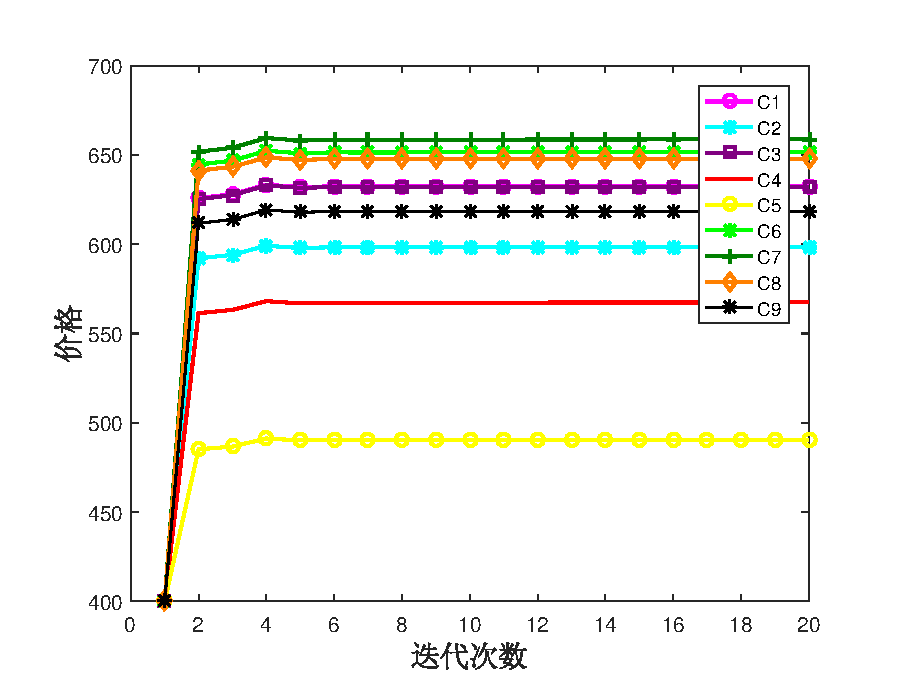
\includegraphics[width=10cm]{figures//chap2//价格.eps}
\caption{价格收敛性能}
\label{价格收敛性能}
\end{figure}

为了进一步验证所提算法的性能,图 \ref{中断概率对此} 和图 \ref{传输速率对比} 完成了对系统鲁棒性和传输速率的验证。在复杂的通信场景中,严重的多用户干扰会影响用户的信号传输,甚至造成中断。
\begin{figure}[H]
\centering
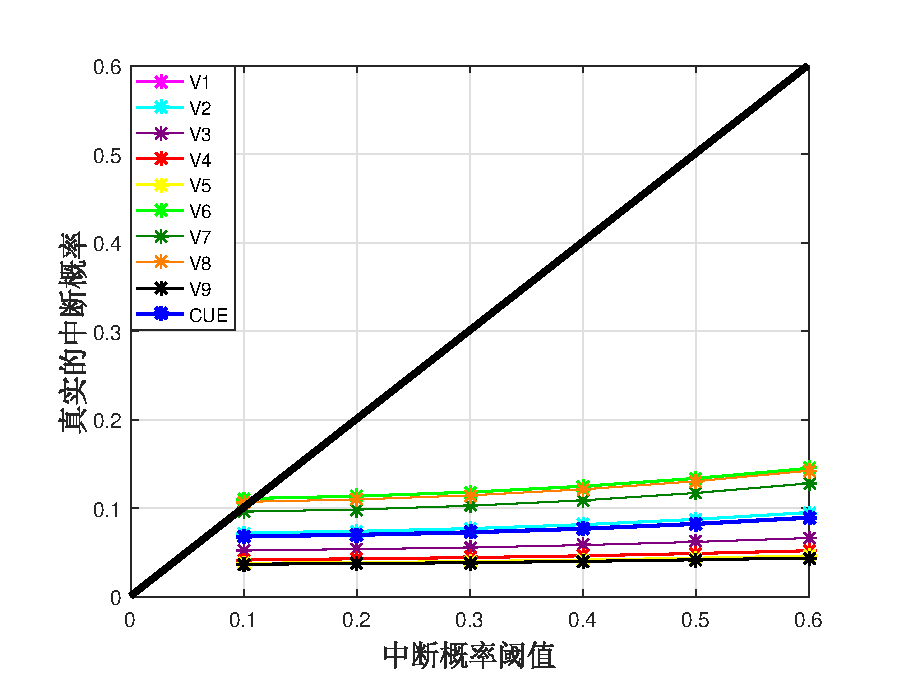
\includegraphics[width=10cm]{figures//chap2//中断概率.eps}
\caption{中断概率对此}
\label{中断概率对此}
\end{figure}
\begin{comment}
\begin{figure}[H]
\centering
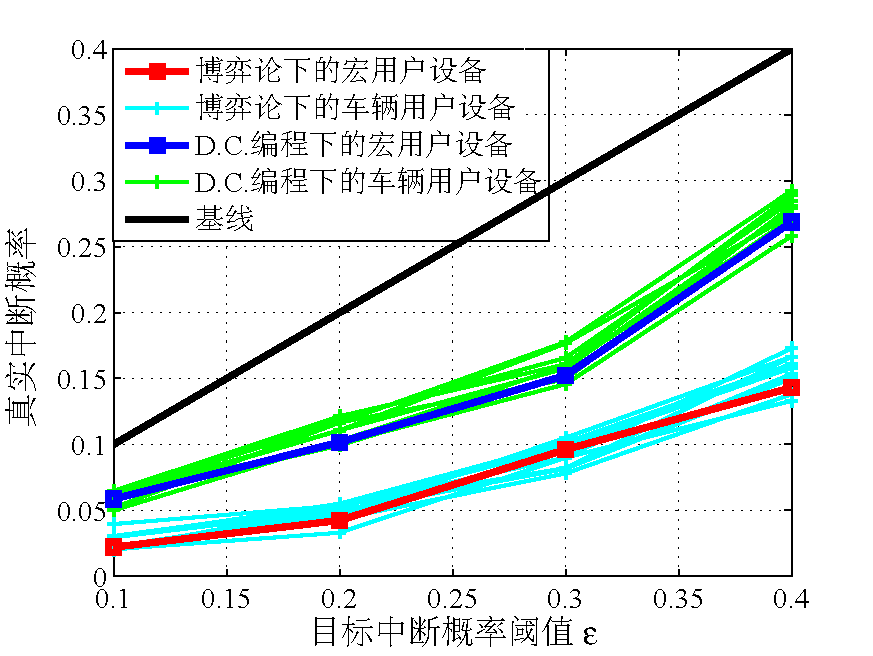
\includegraphics[width=10cm]{figures//chap2//4.pdf}
\caption{中断概率对此}
\label{F44}
\end{figure}
\end{comment}
如图 \ref{中断概率对此} 所示,当真实的阈值 $\varepsilon$ 在 0.1 到 0.6 之间变化时,用户的实际中断概率总是小于给定的阈值。结果证实,本章方法不仅实现了有效的干扰管理,还保证了传输的鲁棒性。
%通过与 \cite{PCID}和基线(目标和实际中断概率相等)比较,本章所有用户的实际中断概率都是低于基准值的。这进一步
说明本文提出的基于鲁棒博弈的算法在信道不确定性较高的实际场景中更加稳定。
\begin{figure}[H]
\centering
\includegraphics[width=10cm]{figures//chap2//传输速率对比.eps}
\caption{传输速率对比}
\label{传输速率对比}
\end{figure}

如图 \ref{传输速率对比} 所示,在不同的方案对比时,博弈论方法中的
%本文中 CUE 和 VUE 的传输速率比 \cite{PCID}和 \cite{ACAR}更均衡。这是因为本章构建了一个非合作博弈框架,在这个框架中,VUE 都是自私的,都在为自己的利益而竞争。在原问题 \eqref{E2-14}和 \eqref{E2-15}中,
价格是实现 VUE 之间平衡的关键变量。当一个 VUE 通过增加功率来提高传输速率时,它将受到来自 BS 的更
多干扰费的惩罚。通过多轮博弈,每个用户都达到了自己最满意的状态,因此用户的传输速率得到了很好的平衡,也高于文献 \cite{Ren2015}中使用的方法和 使用二分法的传输速率。

图 \ref{不同车辆} 表示了三种不同的方案下,%随着系统中车辆数量的增加,
每辆车的平均传输速率。
\begin{figure}[H]
\centering
\includegraphics[width=10cm]{figures//chap2//不同车辆.eps}
\caption{不同车辆时系统的平均传输速率}
\label{不同车辆}
\end{figure}

从图 \ref{不同车辆} 可以看出,当车辆数量增加时,
会对车联网系统中的车辆通信的平均传输速率产生一定的消极影响,所提出的鲁棒博弈论的方案在受到系统中越来越多车辆干扰时也能保持
较高的传输速率。%\textcolor[RGB]{202,12,22}{需要添加一点}。
\section{本章小结}\label{section2-5}
在章节中,提出了一种基于博弈的鲁棒的资源分配算法,以实现 AGHVN 中的有效信息传输。该算法以用户间的博弈关系为核心,制定了实时功率分配和定价策略,
在所提出的优化方案中实现了用户利益的最大化。具体而言,为了保证系统的鲁棒性,引入了概率约束,以确保用户服务的可靠性和稳定性。由于信道不确定性的存在,
概率形式非凸且难以处理,因此在凸优化过程中采用了指数积分法。根据仿真结果,功率值和价格在几步内收敛到最优值。还可以得出结论,斯塔克尔伯格博弈优化方
案表现出更好的鲁棒性。因此,所提出的基于鲁棒博弈的资源分配算法在具有复杂多用户干扰和信道不确定性的空地一体化异构车载通信场景下是有效的。
























\begin{comment}
\begin{verbatim}
\begin{figure}[hptb!]
  \centering\small
  \begin{minipage}[t]{0.5\linewidth}
    \centering
    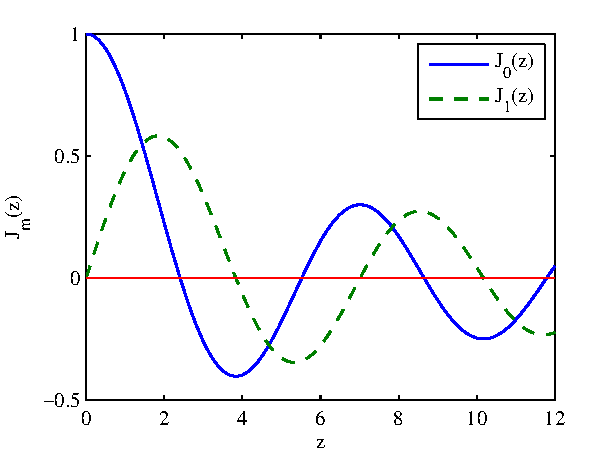
\includegraphics[width=\textwidth]{chp-2_bessel_j}
    (a) 子图a图题
  \end{minipage}%
  \begin{minipage}[t]{0.5\textwidth}
    \centering
    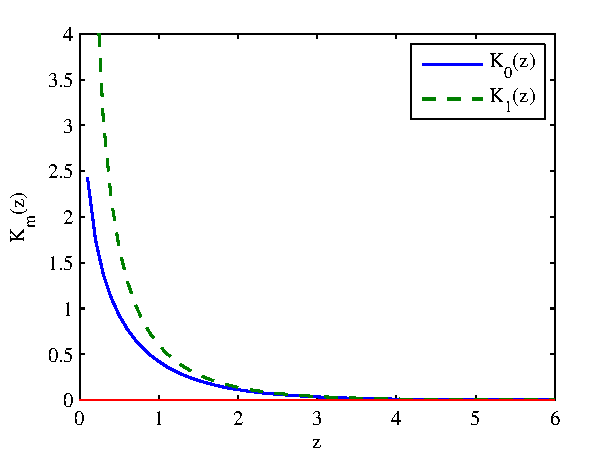
\includegraphics[width=\textwidth]{chp-2_bessel_k}
    (b) 子图b图题
  \end{minipage}  \\
  \begin{minipage}[t]{0.5\textwidth}
    \centering
    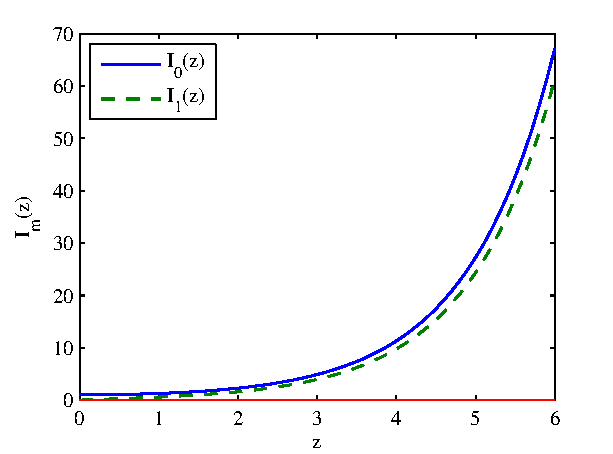
\includegraphics[width=\textwidth]{chp-2_bessel_i}
    (c) 子图c图题子图c图题子图c图题
  \end{minipage}%
  \begin{minipage}[t]{0.5\textwidth}
    \centering
    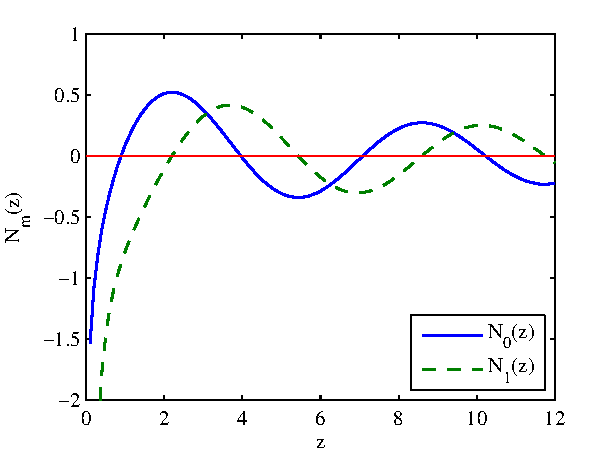
\includegraphics[width=\textwidth]{chp-2_bessel_n}
    (d) 子图d图题子图d图题子图d图题
  \end{minipage}
\Figcaption{贝塞尔函数}  \label{fig-bessel-function}
\end{figure}
\end{verbatim}
注意其中与一对并排图形不同的地方,加入了换行命令“$\backslash\backslash$”。
最终效果如图\ref{fig-bessel-function}所示。
\begin{figure}[hptb!]
  \centering\small
  \begin{minipage}[t]{0.5\linewidth}
    \centering
    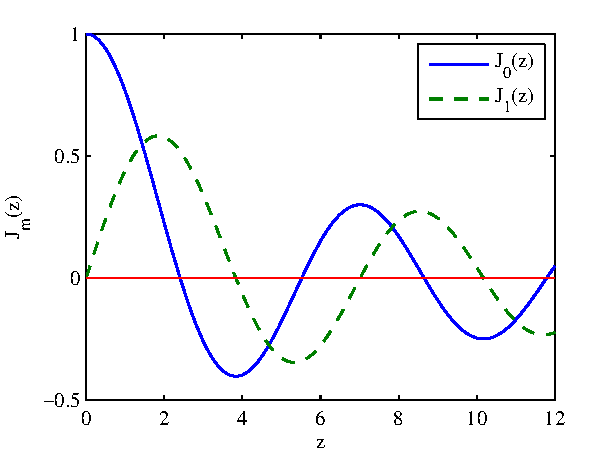
\includegraphics[width=\textwidth]{chp-2_bessel_j}
    (a) 子图a图题
  \end{minipage}%
  \begin{minipage}[t]{0.5\textwidth}
    \centering
    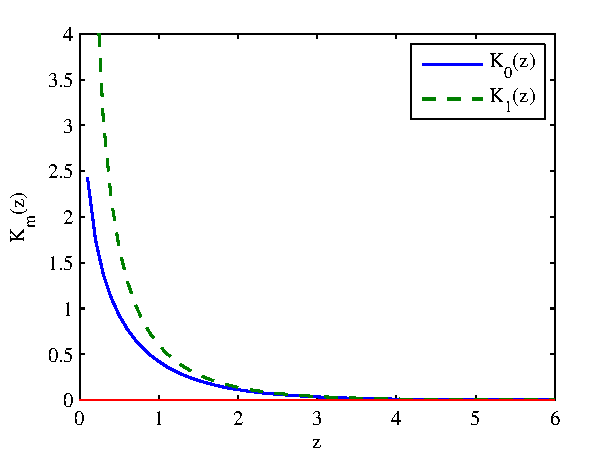
\includegraphics[width=\textwidth]{chp-2_bessel_k}
    (b) 子图b图题
  \end{minipage}  \\
  \begin{minipage}[t]{0.5\textwidth}
    \centering
    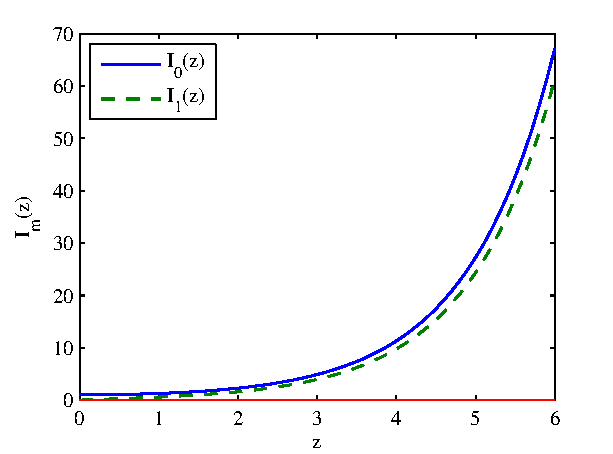
\includegraphics[width=\textwidth]{chp-2_bessel_i}
    (c) 子图c图题子图c图题子图c图题
  \end{minipage}%
  \begin{minipage}[t]{0.5\textwidth}
    \centering
    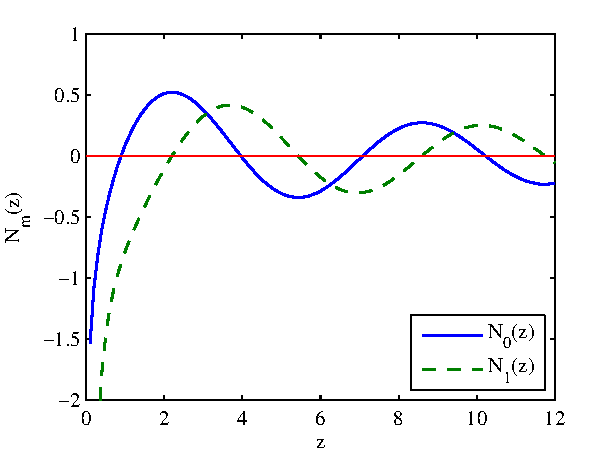
\includegraphics[width=\textwidth]{chp-2_bessel_n}
    (d) 子图d图题子图d图题子图d图题
  \end{minipage}
\Figcaption{贝塞尔函数}  \label{fig-bessel-function}
\end{figure}

其它类似的多个图形并排或者堆叠均可以灵活的运用minipage照猫画虎获得。

\section{图题}\label{section2-4}
其实上边的例子中已经包含了图题的引用命令\verb|\Figcaption|。
例如图\ref{fig-bessel-function}中:
\begin{verbatim}
    \Figcaption{贝塞尔函数}\label{fig-bessel-function}
\end{verbatim}
为当前的图形添加中文图题“贝塞尔函数”。同时添加标签“fig-bessel-function”。对图形的引用就是通过标签来实现的。

\section{图形的引用}\label{section2-5}
在已知图形的标签的基础之上,通过命令:
\begin{verbatim}
\ref{label}
\end{verbatim}
来引用标签为“label”的图形。\LaTeX 会自动将其替换为图形的编号。例如:
\begin{verbatim}
贝塞尔函数的图形如图\ref{fig-bessel-function}所示。
\end{verbatim}
的效果如下:\\
贝塞尔函数的图形如图\ref{fig-bessel-function}所示。


\section{本章小结}\label{section2-6}
注意!从第二章开始应有``本章小结",主要总结本章所做的主要研究工作,研究成果等内容!!!

%

\end{comment}


% !Mode:: "TeX:UTF-8"
\chapter{云辅助的车辆网络功率控制与任务卸载} \label{chap:table 第三章}  %\cite{yaojianquan2009}

\section{引言}\label{section3-1}
云辅助移动边缘计算(C-MEC)为车载网络提供了丰富的计算资源,是一种前景广阔的任务卸载解决方案。本章提出了一种鲁棒的功率
控制和任务卸载方案,以卸载计算任务并最大化 C-MEC 网络的效用。然而,不确定的信道状态会严重影响卸载任务的传输稳定性。为
了模拟信道的不确定性,采用了一阶马尔可夫过程,并考虑了车辆的移动性。此外,由于频谱资源有限,假设信道重用会导致复杂的同
信道干扰。为了克服这些限制,对信号链路实施了概率约束,以确保通信质量。采用伯恩斯坦近似法将原始约束转化为可解约束。此外,
还进一步采用了块坐标下降(BCD)方法和连续凸近似(SCA)技术来解决非凸鲁棒性优化问题。为确定最优解,提出了一种鲁棒功率控
制和任务卸载调度算法。对提出的算法进行了数值仿真,以评估系统的性能。结果表明,与基准模型相比,该算法非常有效,尤其是在
信道不确定的通信环境中。移动边缘计算(MEC)和移动云计算(MCC)作为新兴的5G 网络的两种新架构,通常用于支持物联网设备的任
务卸载、特别是提供低延迟、高可靠性的计算服务。MEC 可以充当网络中心边缘的云服务提供商,提供存储、图像、缓存和第三方访问
功能,这不仅减轻了无线网络的带宽压力,还提供了低延迟、高可靠性的计算服务 \cite{基于车辆边缘计算的任务卸载策略研究}。
并且MEC 在网络中心的边缘,可以减少传输延迟,并为车辆分配计算资源,以缓解计算压力 \cite{CCO}。 然而,当计算任务要求较高时,
MEC 的计算资源仍显不足。由于高性能计算由云服务器提供,基于云的计算网络已被部署以满足爆炸式增长的计算卸载需求 \supercite{Towards2024,SurveyMEC2017,SurveyMEC2018,DistributedTask2024}。
然而,云计算中心往往远离主干道,导致云计算延迟较长并造成网络拥堵与隐私泄露等问题 \supercite{Qian2023, 曹宇慧车载边缘计算环境下任务协同卸载方法研究,云计算隐私10418975}。
在高动态车联网中,车辆传输的数据必须实时处理。因此,在网络架构中部署C-MEC,以提供丰富的计算资源并减少传输延迟。

本章提出了一种鲁棒的云功率控制和任务卸载算法,以辅助高动态车辆网络中的 MEC。 与现有的功率控制或资源分配计算方面的单边研
究不同,本章研究了一个非常强调协作的网络系统,并通过满足概率约束保证了通信延迟和计算延迟;在该框架中,车辆的服务质量(QoS)
也得到了保证。 综上所述,本章的主要贡献可概述如下:
%\begin{itemize}
%\item

(1) 考虑了用于计算卸载架构的实用 C-MEC 车辆网络。 由于 MEC 层部署在网络附近并具有计算能力,因此 MEC 层可作为车辆与云服务器之间的桥梁。 云计算层处理 MEC 层无法处理的对延迟不敏感的大规模数据。 这种网络结构缩短了传输时间,并提供了大量的计算资源。

(2) 采用一阶马尔可夫过程来处理 C-MEC 车辆网络环境高速移动引起的信道不确定性。 为了模拟C-MEC 车载网络的动态特性,采用Bernstein 方法逼近大规模动态车载网络环境中的非凸中断约束。

(3) 提出了一种处理传输任务的高效结构,并开发了一种鲁棒的功率控制和任务卸载调度算法,以接近最优解。 在 C-MEC 车辆网络下,当任务发起车辆无法独立完成任务时,利用 V2R 传输来减少延迟。 模拟验证了系统卸载效用的提高。
%\end{itemize}
\section{系统模型与问题描述}\label{section3-2}
本文研究的C-MEC 车载网络如图 \ref{F1} 所示,由MEC 层和云计算层分层计算卸载架构组成。众多车辆在RSU 的覆盖范围内被划分为多个地理区域,每个RSU 下覆盖一个小区,每个RSU 配备一台MEC 服务器,为车辆提供计算卸载服务。我们将移动系统中的两组车辆和MEC 服务器分别记为$\mathcal{V}=\left\{1,2,..., V\right\}$ 和$\mathcal{M}=\left\{1,2,..., M\right\}$。 高速移动无线通信链路称为 V2RSU (V2R)链路,固定有线连接链路称为 RSU 到云(R2C)链路。详细的卸载过程描述如下。首先,车辆通过无线接口向云发送卸载请求信息,其中包括所需的通信资源、任务 ID 和提交时间,以及任务的最大可容忍服务时间。其次,MEC 服务器根据接收到的请求信息进行调度,包括任务上传服务器和任务计算服务器。最后,任务上传后,任务被推送到服务器队列中,直到服务器执行任务。
% 此外,本文中使用的一些术语如表所示。
\begin{figure}[H]
\centering
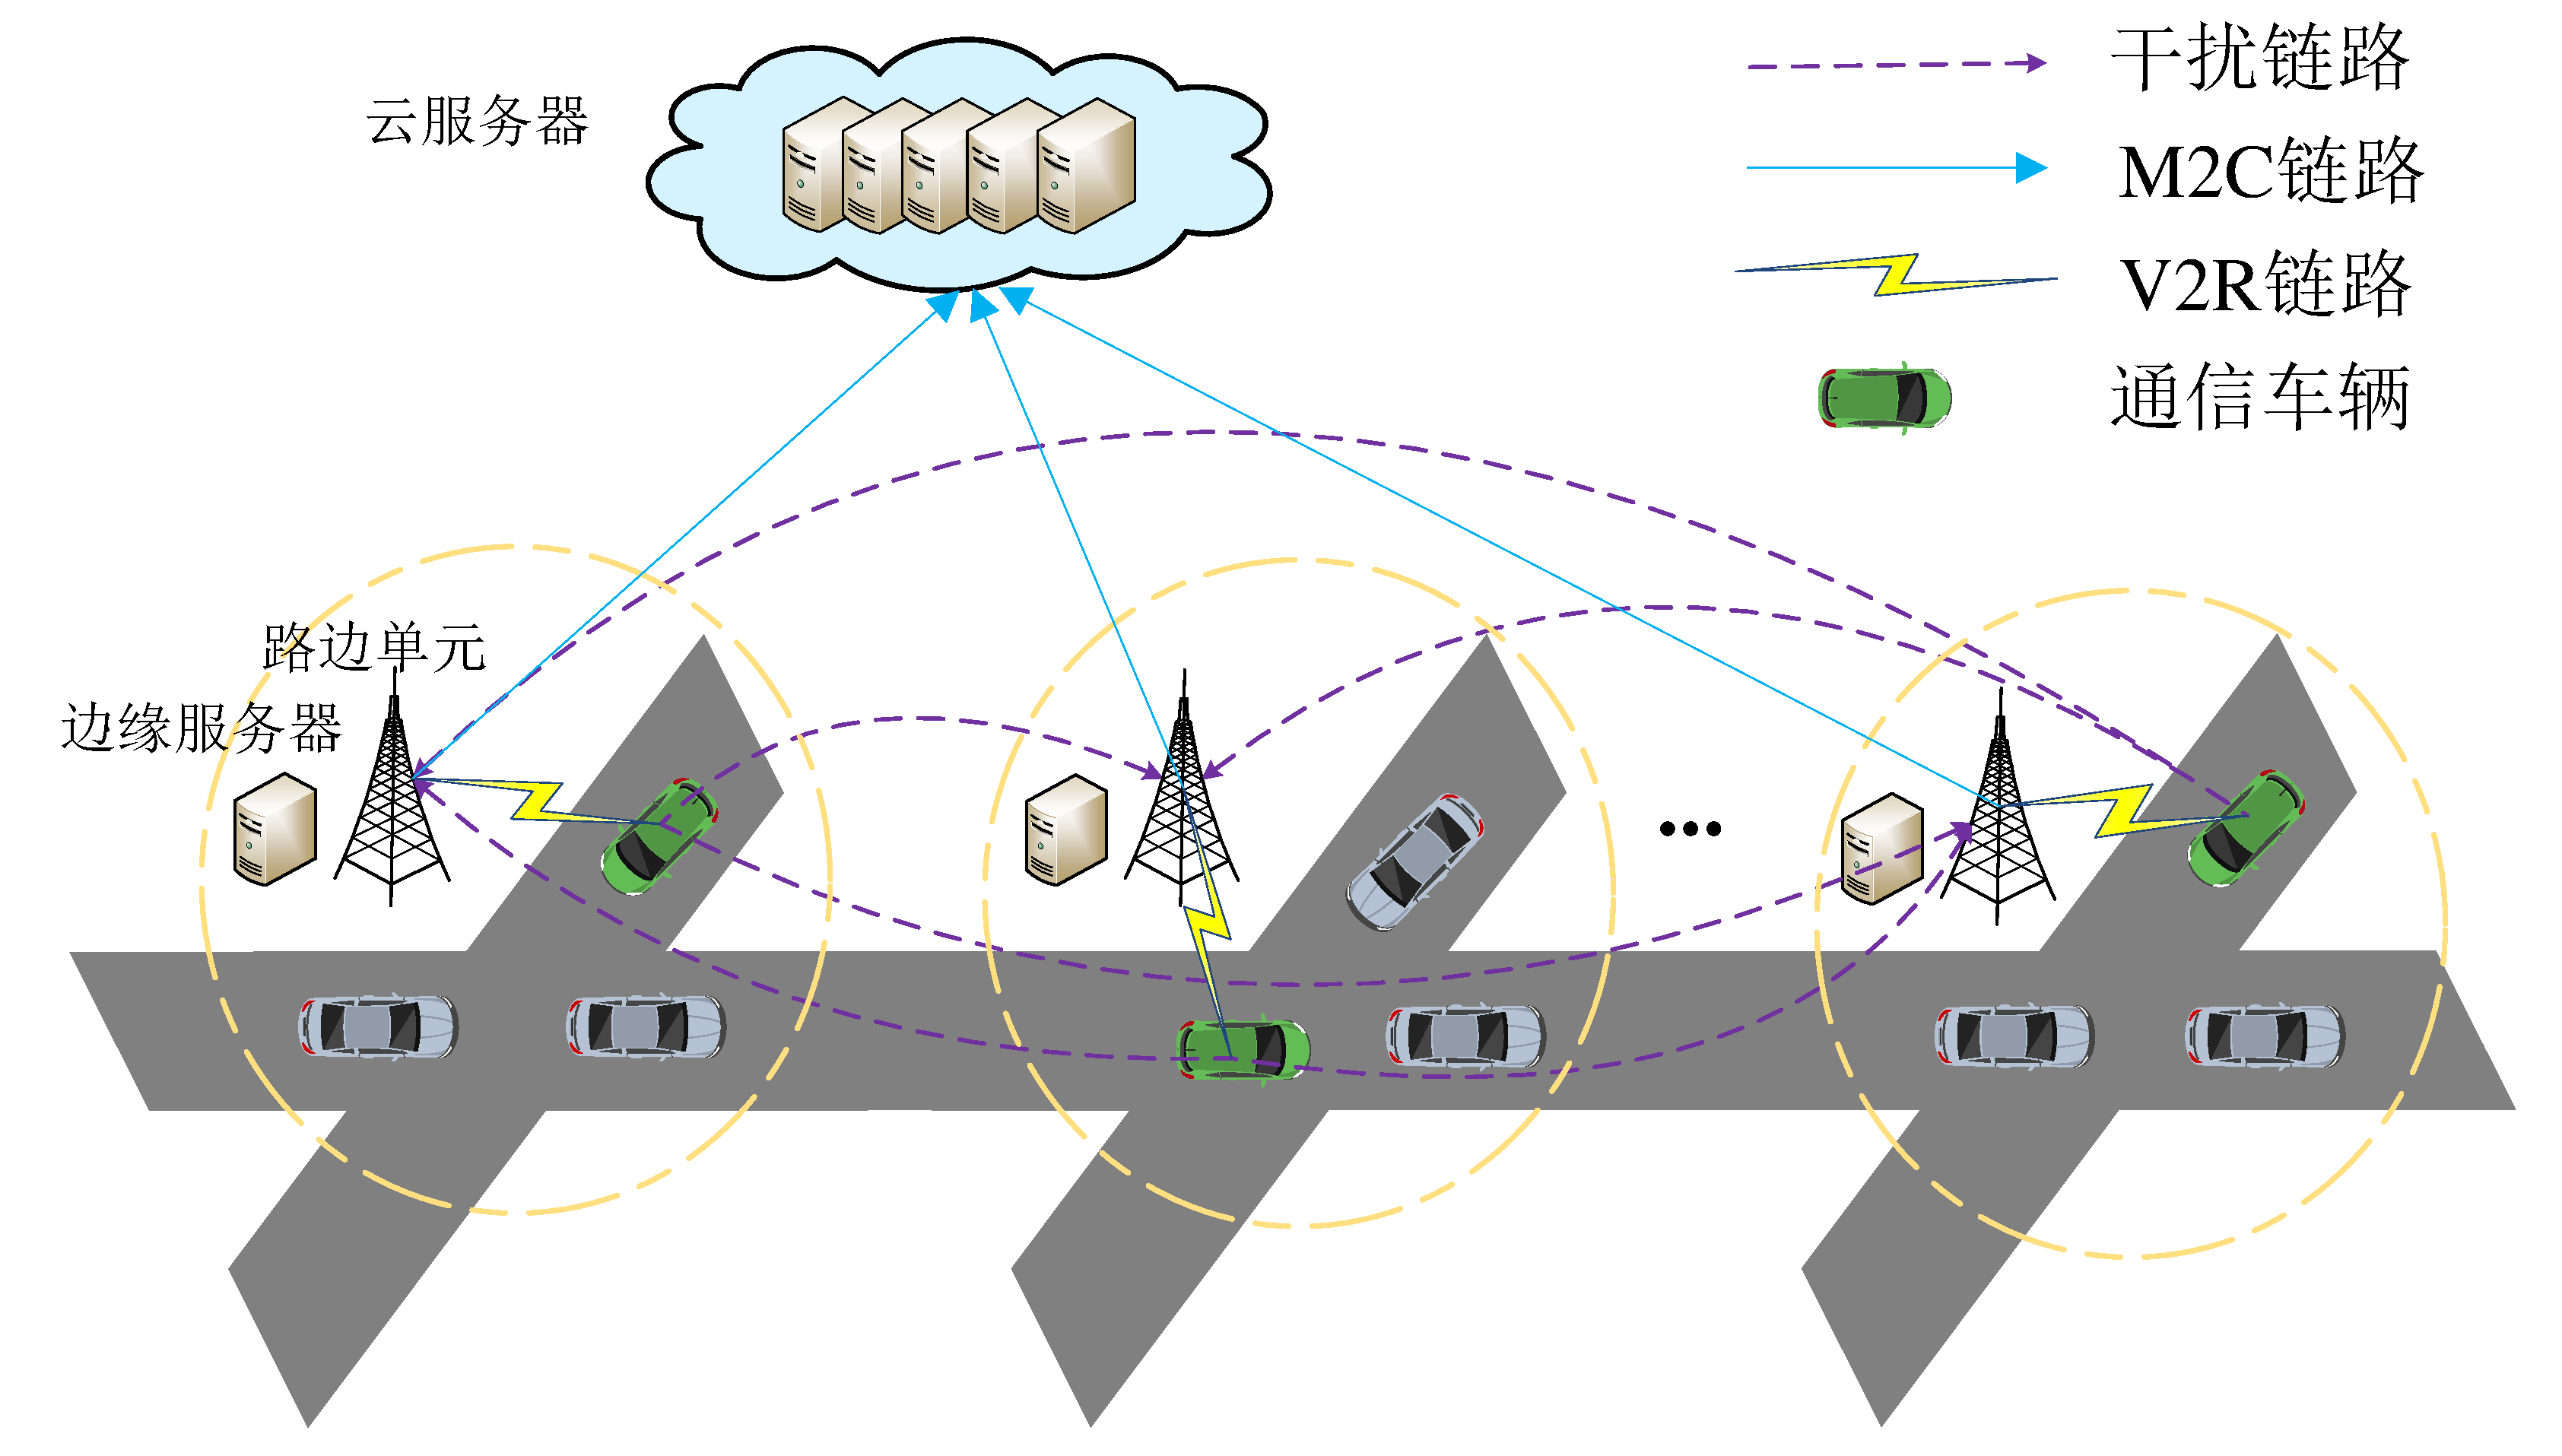
\includegraphics[width=12cm]{figures//chap3//文章一在用model2.pdf}
\caption{C-MEC 系统模型图}
\label{F1}
\end{figure}

\subsection{通信模型}\label{section3-2-1}
由于车辆移动速度快,通信模式与传统的蜂窝通信不同。因此,很难直接获得 CSI。 其中,RSU 仅能准确获取车辆到 RSU 链路的大尺度衰落 $L^2$,而小尺度衰落 $h$ 受多普勒效应引起的快速信道变化影响较大。我们假设CSI 是通过信道估计获得的,因此,我们利用一阶高斯- 马尔可夫过程\cite{Kim2011} 对每个传输时间间隔内的小尺度衰落信道估计$h$ 建模如下,
\begin{eqnarray}\label{E1}
h=\xi{\widetilde{h}}+\sqrt{1-\xi^2}\zeta
\end{eqnarray}
我们假设估计的信道增益 $\widetilde{h}$ 表示对 $h$ 的估计,${\widetilde{h}}^2$ 是指数分布,具有单位平均值\cite{Sakr2014}。 此外,$\xi\in\left(0,1\right)$ 表示 V2R 链路上的相关系数,$\zeta$ 表示信道增益,其复高斯分布为 $\zeta\sim CN\left(0,\delta^2\right)$ ,与 $\widetilde{h}$ 无关。系数$\left(0<\zeta<1\right)$ 量化了两个连续时隙之间的信道相关性,我们假设所有车辆都存在相同的时间相关系数$\zeta$。Jakes 的衰落信道统计模型\cite{Kim2011} 指出:$\zeta=J_0\left(2\pi f_{max}T_s\right)$ ,其中$J_0$ 是第一类零阶贝塞尔函数。$f_{max}=\bar{\nu}f_c/c $ 是最大多普勒频率,其中 $\bar{\nu}$ 表示车辆速度,$f_c$ 表示 5.9 Ghz 的载波频率,$c=3\times{10}^8$m/s,$T_s$ 是周期反馈延迟。发射车和 RSU 都知道实际的 $\zeta$。

根据上述讨论,从第$ i$ 个车辆发射器到第 $j $ 个接收器的第$ k $ 个时隙内,有效链路和干扰链路的移动 V2R 信道功率增益用共享表达式表示:
\begin{eqnarray}\label{E2}
G_{i,j}^k={\widetilde{g}}_{i,j}^k+{\hat{g}}_{i,j}^k
\end{eqnarray}
其中 ${\widetilde{g}}_{i,j}^k=L_{i,j}^2{\widetilde{h}}_{i,j}^2\xi_{i,j}^2$ , ${\hat{g}}_{i,j}^k=L_{i,j}^2\left(1-\xi_{i,j}^2\right)\zeta_{i,j}^2\ $ ,$ {L_{i、 j}^k}^2 $
表示第 $k $ 个时隙的大规模衰减效应,包括阴影衰减和从道路上第 $i$ 个车辆发射器到第 $ j $ 个接收器的路径损耗。此外,${\hat{g}}_{i,j}^k$ 是观测值,${\widetilde{g}}_{i,j}^k$ 表示指数随机变量,参数为 $\frac{1}{L_{i,j}^k}^2({1-{\zeta_{i,j}^k}^2}) $ ,该参数基于 \cite{Xie2020}。

为了提高频谱利用率并实现多车联合通信,V2R 通信重复使用同一上行链路信道。换句话说,车辆 $j$ 和车辆 $i$ 共享同一个上行链路信道,从而导致它们之间产生干扰。在这种情况下,V2R 链路的信号干扰加噪声比(SINR)计算公式为,
\begin{eqnarray}\label{E3}
%\gamma_i\left(\mathbf{p}\right)=\frac{p_ig_{i,j}}{{\sum_{j=1,j\neq i}^{M}{p_jg_{j,i}}+\sigma^2}},
\gamma_i\left(\mathbf{p}\right)=\frac{p_ig_{i,m}}{{\sum_{j=1}^{M}{p_jg_{j,m}}+\sigma^2}}, m=1,2,\cdots ,M , i\in {{\mathcal{V}}_{m}}
\end{eqnarray}
% 其中,$p_j$ 表示第 j 个发射器车辆的发射功率,$\sigma^2$ 为背景噪声。因此,根据香农定理计算出车辆的确定性等效传输速率为,
其中,$g_{i,m}$ 表示 $i_{th}$ 车辆对其集群 RSU 的功率增益,而 ${p_jg_{j,m}}$ 表示其他集群车辆对当前 RSU 的干扰。
\begin{eqnarray}\label{E4}
%{R_i\left(\mathbf{p}\right)=\log}_2{\left(1+\frac{p_ig_{i,j}}{\sum_{j=1,j\neq i}^{M}{p_jg_{j,i}}+\sigma^2}\right)}.
{R_i\left(\mathbf{p}\right)=\log}_2{\left(1+ \gamma_i\left(\mathbf{p}\right) \right)}
\end{eqnarray}
当输入参数为 $d_{i,up}$ 时,车辆 $i$ 向上行链路发送任务输入时的传输时间定义为 $t_{i,up}$。

因此,每个 V2R 链路的上传时间可表述为,
\begin{eqnarray}\label{E6}
t_{i,up}=\frac{d_{i,up}}{WR_i\left(\mathbf{p}\right)}
\end{eqnarray}
其中,$W$ 表示多个 V2R 链路重复使用的信道带宽,$d_{i,up}$ 表示输入数据的大小,包括系统设置、程序代码和输入参数,这些数据是程序执行时必须传输的。

% 通信传输延迟是影响车载网络性能的一个重要因素 \cite{RAI}。 到 RSU 的数据包在传输前必须进入队列,其中传输速度为 $R_i$。 第i 个V2R 接收器的数据包到达过程遵循参数为$k_i$ 的泊松过程,数据包长度为参数为$\tau_i$ 的指数分布。由于基于$M/M/1$ 队列的方法可以保证车辆通信的可靠性,我们利用$M/M/1$ 模型对系统进行分析,并将预期时延表示为第i 条V2R 链路传输速率的函数,其表达式如下,  \cite{liu2021}
通信服务延迟严重影响了车载网络的性能 \cite{RAI}。 为确保高效传输,数据包在传输到 RSU 之前必须排队。 传输速度(用 $R_i$ 表示)受两个参数的影响:数据包到达过程和数据包长度。  第i 个V2R 接收器的数据包到达过程遵循参数为$k_i$ 的泊松过程,数据包长度为参数为$\tau_i$ 的指数分布。 由于基于$M/M/1$ 的排队方法可以保证车辆通信的可靠性 \cite{Guo2019},因此我们利用$M/M/1$ 模型对系统进行分析,并将预期时延表示为第$i$ 条V2R 链路传输速率的函数,其表达式如下、
\begin{eqnarray}\label{E7}
D_i=\frac{1}{{\tau_iR}_i-k_i}
\end{eqnarray}

\subsection{车辆计算模型}\label{section3-2-2}
我们将处理车辆 $i$ 的 1 位输入数据所需的 CPU 周期数表示为 $c_0$ \cite{Zhang2017},它不可分割,无法分解为更小的组件 \cite{Saleem2021}。
我们认为,在$ \mathcal{V}$ 中,每辆车每次都有不同的计算任务,记作 $T_i$,由两个参数组成的元组来定义,即 $\langle d_{i,up}, c_{i,e}\rangle$,其中 $c_{i,e}$ [cycles] 指定了工作量 \cite{Tran2019}。 因此,完成任务的计算成本 $c_{i,e}$ 可以通过 $c_{0}*d_{i,up}$ 得到。每个任务都被卸载到 MEC 服务器,然后传输到云服务器。通过将计算任务卸载到 MEC 服务器,车辆可以获得更多计算资源。然而,在上行链路方向传输任务输入可能会消耗额外的时间。

每个 RSU 上的 MEC 服务器按时段为车辆提供计算卸载服务。计算资源由固定速率 $\bar{f}$ (即每秒 CPU 周期数)量化。第 $i $ 辆车将每个任务的输入数据上传到最近的 RSU。RSU 首先处理小规模、对延迟敏感的数据,然后将剩余数据转发给远程云服务器。{云服务器同时为多个 RSU 提供计算服务。RSU 可用的计算资源取决于从云服务器分配的计算速率 $f_i$,}即每秒 CPU 周期数。因此,计算卸载造成的延迟可计算为,
\begin{eqnarray}\label{E8}
t_{i,exe}=\frac{c_{i,e}}{\bar{f}+f_i}
\end{eqnarray}
\subsection{功率控制与任务卸载问题的定义}\label{section3-2-3}
\begin{comment}
\begin{table}[htbp!]
 \centering\small
 \Tablecaption{燕山大学硕士学位论文参考文献规则}\label{tab:ysubof}
\begin{tabular}{llr}
 \toprule
    论文版本    & 参考文献标准    & 实施年份(年)  \\
 \midrule
    旧版        & BF7714-87       & 1987            \\
    新版        & GBT7714-2005    & 2005            \\
 \bottomrule
 \end{tabular}
\end{table}
\end{comment}
如果计算速度为 $f_i$,则车辆 $i$ 因卸载而产生的总延迟时间为,
\begin{eqnarray}\label{E9}
 t_i=\frac{c_{i,e}}{\bar{f}+f_i}+T_c
\end{eqnarray}
其中,云服务器和 RSU 之间的传输延迟定义为 $T_c$,通常设为一个常量 \cite{Xiao2020}。 因此,任务完成时间的相对效用函数的特征为,
\begin{eqnarray}\label{E10}
U_{i,exe}=\frac{t_{max}-t_{i,exe}}{t_{max}}
\end{eqnarray}
其中,$t_{max}$ 为{任务完成可容忍阈值的最长时间}。换句话说,当任务同时在 MEC 服务器和云上执行时,每辆车都能通过最小化任务执行时间获得更大的效用。否则,就会产生相应的损失。因此,车辆 $i$ 的卸载效用定义为 $\frac{U_{i,exe}}{t_{i,up}}$,即单位时间内的卸载效用函数。

本节将功率控制和任务卸载表述为一个优化问题,试图最小化网络中所有车辆由延迟和传输速率组成的总系统成本。给定上行链路功率分配向量 $\mathbf{p}$ 和计算速率向量 $\mathbf{f}$ 后,系统效用被定义为所有车辆卸载效用的加权和。
\begin{eqnarray}\label{E12}
U=\sum_{i=1}^{M}\frac{U_{i,exe}}{t_{i,up}}
\end{eqnarray}
其中,$U$ 是更大的执行时间效用,上传时间成本较小。我们将鲁棒优化问题,即功率控制和任务卸载问题,表述为系统效用最大化问题,
\begin{align}
 &\qquad\qquad\max\limits_{\mathbf{p},\mathbf{f}}\sum_{i=1}^{M}\frac{U_{i,exe}}{t_{i,up}}                                   \label{E3-13}\\
\text { s.t. }
& \textrm{Pr}\left\{\gamma_i\geq\gamma_{th}\right\}\geq1-\varepsilon_1                                         \tag{\ref{E3-13}{-1}}      \label{E3-13-1}\\  % 信噪比中断概率约束
& \textrm{Pr}\left\{\frac{1}{\tau_iR_i-k_i}+\frac{c_{i,e}}{\bar{f}+f_i}\le D_{max}\right\}\geq1-\varepsilon_2  \tag{\ref{E3-13}{-2}}      \label{E3-13-2}\\  % 功率阈值
& \sum_{i=1}^{N}f_i\le f_{total}                                                                                \tag{\ref{E3-13}{-3}}      \label{E3-13-3}\\  % 时隙分配加起来是一
& \le p_i\le p_{max}                                                                                          \tag{\ref{E3-13}{-4}}      \label{E3-13-4} % 这个是时隙的约束
\end{align}
%& q_U^{n\mathrm{\ }+1}-q_U^{n\mathrm{\ }}\le tV_{max}, \forall m         \tag{\ref{E2-13end}{-5}}      \label{E2-13end5}    % 无人机飞行轨迹
其中,$U$ 表示网络效用。\eqref{E3-13} 中的约束条件解释如下: 约束条件 \eqref{E3-13-1} 保证了车辆的 QoS 要求。然而,网络拓扑结构的时变会导致大量计算。在车辆通信场景中,实时 SINR 难以量化获取。由于 CSI 反馈的时间间隔非常小,因此用长期 SINR 代替实时 SINR。 我们用 $\gamma_i$ 表示第$i$ 个 V2R {链路的平均 SINR,使用较小的 CSI 反馈时间间隔}。为确保任务成功卸载到 RSU,SINR 必须大于 SINR 阈值 \cite{liu2021}。$\gamma_{th}$ 是检测 V2R 链路通信的 SINR 阈值。$\textrm{Pr}\left\{\cdot\right\}$ 定义了输入 SINR 的概率。中断概率约束保证了车辆链路的可靠性。$D_{max}$ 表示第 $i$ 个 V2R 链路在数据传输过程中允许的最大延迟。此外,$\varepsilon_1$ 和$\varepsilon_2$ 分别是与SINR 和延迟约束相关的中断概率阈值,其中$\varepsilon_1,\varepsilon_2\in\left(0,1\right)$。 约束 \eqref{E3-13-2} 表示通信和计算的总延迟大于延迟阈值。约束 \eqref{E3-13-3} 确保云服务器必须为与其相关联的 RSU 分配计算资源,约束 \eqref{E3-13-3} 还确保分配给所有相关联 RSU 的总计算资源不得超过云服务器的计算能力。因此,特定边缘云所服务的应用数量必须低于其容量。在约束条件 \eqref{E3-13-4} 中,$p_{max}$ 是车辆通信网络中发射车辆的最大发射功率,且发射功率大于零。

\begin{comment}
实现代码如下:
\end{comment}
\section{功率控制与任务资源分配问题的求解}\label{section3-3}
在本节中,我们提出了一种基于 BCD 的算法来求解优化问题 \eqref{E3-13}。BCD 方法将复杂的原问题分解为一系列较简单的子问题。BCD 方法首先将所有变量分成两块,交替优化。

为了解决 \eqref{E3-13} 问题,可以通过固定计算率向量 $\mathbf{f}$ 的优化变量来优化问题。该问题通过交替优化两个子问题来解决。去掉向量 $\mathbf{f}$ 后,问题 \eqref{E3-13-1} 可以转化为下面的问题,
\begin{align}
& \textbf{P1}:\qquad\max\limits_{\mathbf{p}}\sum_{i=1}^{M}\frac{U_{i,exe}}{t_{i,up}}                                  \label{E3-14}\\
\text { s.t. }
& \textrm{Pr}\left\{\gamma_i\geq\gamma_{th}\right\}\geq1-\varepsilon_1                                         \tag{\ref{E3-14}{-1}}      \label{E3-14-1}\\  % 信噪比中断概率约束
& \textrm{Pr}\left\{\frac{1}{\tau_iR_i-k_i}+\frac{c_{i,e}}{\bar{f}+f_i}\le D_{max}\right\}\geq1-\varepsilon_2  \tag{\ref{E3-14}{-2}}      \label{E3-14-2}\\  % 功率阈值
& 0\le p_i\le p_{max}                                                                                          \tag{\ref{E3-14}{-3}}      \label{E3-14-3}  %\\  % 时隙分配加起来是一
%& 0\le p_i\le p_{max},                                                                                          \tag{\ref{E3-13}{-4}}      \label{E3-13-4} % 这个是时隙的约束
%& q_U^{n\mathrm{\ }+1}-q_U^{n\mathrm{\ }}\le tV_{max}, \forall m         \tag{\ref{E2-13end}{-5}}      \label{E2-13end5}    % 无人机飞行轨迹
\end{align}

\subsection{目标方程中的连续凸逼近方法}\label{section3-3-1}
由于$t_{i,up}$ 中的香农定理的形式,目标函数\eqref{E3-14} 是对数形式,因此\eqref{E3-14-1} 是一个非凸和非确定多项式困难(NP-hard)问题。这里使用 SCA 方法将问题 \eqref{E3-14-1} 简化为可解问题。利用近似约束来近似原始函数如下,
\begin{eqnarray}\label{E15}
\begin{array}{ll}
\alpha \ln{\left(z\right)}+\beta\le \ln{\left(1+z\right)},\\
\end{array}
\end{eqnarray}
其中 $\alpha=\frac{z_0}{1+z_0}$ 并且 $\beta=\ln{\left(1+z_0\right)}-\frac{z_0}{1+z_0}\ln{\left(z_0\right)}$。 \eqref{E15} 中的每个项都可以通过连续凸近似转换为 $A_k\ln\left(\gamma_k\left(e^{\widetilde{\mathbf{p}}}\right)\right)+B_k$ 。 其中,$A_k$ 和$B_k$ 分别选为$A_k=\gamma_i/\left(1+\gamma_i\right)$ 和$B_k=\ln{\left(1+\gamma_i\right)}-A_k\ln{\left(\gamma_i\right)}$,其中$A_k=1$,$B_k=0$。目标函数的每项都可以写成如下,
\begin{eqnarray}\label{E16}
\frac{1}{\ln{2}}\sum_{i=1}^{M}{\frac{U_{i,exe}}{d_{i,up}}\left.\left[{A_k\ln{\left(\gamma\left(p\right)\right)}+B}_k\right.\right]},
\end{eqnarray}
由于 \eqref{E3-14} 中的目标函数是 SINR 的分数,因此不容易直接计算。因此,我们使用变量替换法,即 ${\hat{p}}_i=\ln{p_i}$,
$p_i=e^{{\hat{p}}_i}$, and ${\hat{p}}_i\le \ln{p_{max}},\ \forall\ \ 1\le i\le M$
\begin{eqnarray}\label{E17}
U=\max\frac{1}{\ln{2}}\sum_{i=1}^{M}\left.\frac{U_{i,exe}}{d_{i,up}}\left[{A_k\ln{\left(\gamma\left(e^{\widetilde{P}}\right)\right)}+B}_k\right.\right]
\end{eqnarray}

\begin{comment}
\begin{table}[htbp!]
\centering\small
\Tablecaption{带有合并列的三线表}\label{tab:test}  % 合并列通常见于表格的第一行,在适当的位置使用\verb|\multicolumn| 命令即可。
\begin{tabular}{llr} \toprule
\multicolumn{2}{c}{Item} \\ \cmidrule(r){1-2}
Animal & Description & Price (\$)\\ \midrule
Gnat & per gram & 13.65 \\
& each & 0.01 \\
Gnu & stuffed & 92.50 \\
Emu & stuffed & 33.33 \\
Armadillo & frozen & 8.99 \\ \bottomrule
\end{tabular}
\end{table}
\end{comment}


\subsection{中断概率的近似}\label{section3-3-2}
\begin{comment}
\begin{table}[htbp!]
\end{comment}
由于 \eqref{E3-14-1} 是不确定的,而目标函数 \eqref{E3-14} 又是一个非凸问题,因此优化 \eqref{E3-14} 十分困难。有必要设计一种复杂度较低的算法来求解 \eqref{E3-14}。 为了描述不确定信道增益,考虑到快速衰落,采用统计约束来描述不确定性 \eqref{E3-14-1}。 为了进一步简化 \eqref{E3-14-1},引入了矩阵形式。信道增益的一般形式描述为:
\begin{eqnarray}\label{E18}
\textrm{Pr}\left\{\left(\textbf{G}_m\right)^Te^{\widetilde{p}}+\sigma^2\le0\right\}\geq1-\varepsilon_1
\end{eqnarray}
其中 $\textbf{G}_m=\left[G_{1,m},G_{2,m},\ldots,-\frac{G_{m,m}}{\gamma_{th}},\ldots,G_{M,m}\right]^T$。
此外,还采用伯恩斯坦方法来近似考虑信道不确定性的概率约束。

%\begin{theorem}
所有 V2R 链路的中断概率表示为 $\textrm{Pr}\left\{\gamma_i\geq\gamma_{th}\right\}\geq1-\varepsilon_1$
可以重新表述为可分离的约束条件,
\begin{eqnarray}\label{E19}
\!\!\!\sigma^2+\!\sum_{i\neq j}^{M}{\chi_{i,j}e^{{\widetilde{p}}_i}}+\sqrt{2\ln\left(\frac{1}{\varepsilon_1}\right)}\left(\sum_{i\neq j}^{M}\left(\sigma_{i,j}\beta_{i,j}p_i\right)^2\right)^\frac{1}{2}\!\!\!\!\!\le0
\end{eqnarray}
其中 $\chi_{i,j}=\mu_{i,j}^+\alpha_{i,j}+\beta_{i,j}+g_{i,j}$. 参数(即 $\sigma_{i,j}$ 和 $\alpha_{i,j}$)在 \cite{CCO} 中被推导为正值。假设 $G_{i,j}$ 的截断分布具有有界范围 $\left[{\widetilde{g}}_{i,j}^k+\alpha_{i,j},{\widetilde{g}}_{i,j}^k+\beta_{i,j}\right]$,${\widetilde{g}}_{i,j}^k$ 是 $G_{i,j}$ 的估计值。常数 $\alpha_{i,j}=\frac{1}{2}\left(b_{i,j}-a_{i,j}\right)$, $\beta_{i,j}=\frac{1}{2}\left(b_{i,j}+a_{i,j}\right)$ 用于将范围归一化为 $\left[-1,1\right]$ 如下,
\begin{eqnarray}\label{E20}
\xi_{i,j}=\frac{G_{i,j}-{\widetilde{g}}_{i,j}^k-\beta_{i,j}}{\alpha_{i,j}}\in\left[-1,1\right]
\end{eqnarray}
%\end{theorem}

在 \eqref{E19} 的最后一项中,变量 $p_i$ 是非线性耦合的。因此,当 $k$ 增加且车辆数量较多时,用伯恩斯坦方法确定一个可接受的良好解 \eqref{E3-14-1} 非常耗时。因此,有必要为 $\mathbb{R}^k$ 中的任意 $\mathbf{x}$ 引入一个 $\ell_2$ 准则近似问题。因此,包含向量 $\mathbf{x}=\left[\sigma_{i,1}\beta_{i,1}p_i,\cdots,\sigma_{i,M}\beta_{i,M}p_i\right]$ 进一步近似为 $\parallel x\parallel_2 \le \parallel x\parallel_1$. \eqref{E3-14} 中的约束条件被进一步表述为 \eqref{E21},复杂度降低,可靠性提高。
\begin{eqnarray}\label{E21}
\sigma^2+\sum_{i\neq j}^{M}{\chi_{i,j}e^{{\widetilde{p}}_i}}+\sqrt{2\ln\left(\frac{1}{\varepsilon_1}\right)}\sum_{i\neq j}^{M}{\left|\sigma_{i,j}\beta_{i,j}\right|e^{{\widetilde{p}}_i}}\le0
\end{eqnarray}

为了得到问题 \eqref{E21} 的简单形式,我们定义,
\begin{eqnarray}\label{E22}
\ \mathrm{\Pi}_i=\sigma^2+\sqrt{2\ln\left(\frac{1}{\varepsilon_1}\right)}\sum_{i\neq j}^{M}{\left|\sigma_{i,j}\beta_{i,j}\right|e^{{\widetilde{p}}_i}}
\end{eqnarray}

利用积分变换法重新表述了约束条件 \eqref{E3-14-2}。 根据约束条件 \eqref{E3-14-2},$X={\widetilde{h}}^2$ 是一个具有单位均值的指数随机变量,即 其中 $D_{max}=D_1+D_2 $,$D_1=\frac{1}{\tau_iR_i-k_i} $,$D_2=\frac{c_{i,e}}{f_i} $。 我们可以确定通信延迟概率的可行功率区域如下,
\begin{eqnarray}\label{E23}
\left.\left[\ln\left(1-\varepsilon_2\right)-{\hat{g}}_{i,j}^k\right.\right]e^{{\widetilde{p}}_i}+D^\ast\ \le0
\end{eqnarray}
证明求解过程如下,
\begin{equation}\label{E24}
\begin{array}{ll}
\qquad\qquad\qquad\qquad\quad\textrm{Pr}\left\{\frac{1}{\tau_iR_i-k_i}+\frac{c_{i,e}}{f_i}\le D_{max}\right\}\\
\qquad\qquad\qquad\qquad\quad=\textrm{Pr}\left\{R_i\geq\frac{1}{R_i\left(D_{max}-D_2\right)}+\frac{k_i}{\tau_i}\right\}\\
\qquad\qquad\qquad\qquad\quad\!\le1\!-\!\textrm{Pr}\left\{p_i{\widetilde{g}}_{i,j}^k\le\left(I_{th}+\sigma^2\right)2^\frac{1+k_i\left(D_{max}-D_2\right)}{\tau_i\left(D_{max}-D_2\right)}-p_i{\hat{g}}_{i,j}^k\right\}\\
\qquad\qquad\qquad\qquad\quad=\!1\!-\!\int_{0}^{\left(I_{th}+\sigma^2\right)2^\frac{1+k_i\left(D_{max}-D_2\right)}{\tau_i\left(D_{max}-D_2\right)}-p_i{\hat{g}}_{i,j}^k}{e^{-x}dx}\!\geq\!1-\varepsilon_2
\end{array}
\end{equation}
不等式函数 \eqref{E24} 等价于 \eqref{E25} 为,
\begin{eqnarray}\label{E25}
\left.\left[\ln\left(1-\varepsilon_2\right)-{\hat{g}}_{i,j}^k\right.\right]e^{{\widetilde{p}}_i}+D^\ast\ \le0
\end{eqnarray}
其中 $D^\ast=\left(I_{th}+\sigma^2\right)2^\frac{1+k_i\left(D_{max}-D_2\right)}{\tau_i\left(D_{max}-D_2\right)}$。

因此,将方程 \eqref{E3-26} 给出的鲁棒功率控制的确定性优化问题进行变换,我们可以将目标函数、停电概率约束和延迟约束重新表述如下:
\begin{align}
&\textbf{P1}:\max\limits_{\mathbf{p}}\frac{1}{\ln{2}}\sum_{i=1}^{M}\left.\frac{U_{i,exe}}{d_{i,up}}
\left[{A_k\ln{\left(\gamma\left(e^{\widetilde{P}}\right)\right)}+B}_k\!\!\right.\right]                         \label{E3-26}\\
\text { s.t. }
& \sum_{i=1}^{M}{\chi_{i,j}e^{{\widetilde{p}}_i}}+\mathrm{\Pi}_i\le0                                           \tag{\ref{E3-26}{-1}}      \label{E3-26-1}\\  % 信噪比中断概率约束
& \left.\left[\ln\left(1-\varepsilon_2\right)-{\hat{g}}_{i,j}^k\right.\right]e^{{\widetilde{p}}_i}+D^\ast\le0  \tag{\ref{E3-26}{-2}}      \label{E3-26-2}\\  % 功率阈值
& -\infty\le{\widetilde{p}}_i\le \ln{p_{i,max}}                                                                \tag{\ref{E3-26}{-3}}      \label{E3-26-3}  %\\  % 时隙分配加起来是一
\end{align}
\subsection{优化功率问题}\label{section3-3-3}
为了解决问题 \eqref{E3-26},我们使用了一种迭代算法,即拉格朗日法,当给出两个系数 $X_i$ 和 $Y_i$ 时,最大化原目标的下限。对这两个系数进行更新,以保证下限性能的单调增长。

因此,具有固定系数 $X_i$ 和 $Y_i$ 的 \eqref{E3-26} 的拉格朗日函数可表述为:
\begin{comment}
\begin{align}\label{E27}  % 没有左对齐的公式
L\left(\widetilde{\mathbf{p}},\lambda,\mu\right)=\frac{1}{\ln{2}}\sum_{i=1}^{M}{\frac{U_{i,exe}}{d_{i,up}}\left[A_k\ln{\left({\bar{\gamma}}_k\left(e^{\widetilde{\mathbf{p}}}\right)\right)}+B_k\right]}\\
\notag-\mu_k\Big[\left(\ln\left(1-\varepsilon_2\right)-{\hat{g}}_{i,j}^k\right)e^{{\widetilde{p}}_i}+D^\ast\Big]\\
-\lambda_k\Big[\sum_{i=1}^{M}{\chi_{i,j}e^{{\widetilde{p}}_i}}{+\mathrm{\Pi}}_i\Big]\notag,
\end{align}
\end{comment}

\begin{align}\label{E27}
L\left(\widetilde{\mathbf{p}},\lambda,\mu\right)&=\frac{1}{\ln{2}}\sum_{i=1}^{M}{\frac{U_{i,exe}}{d_{i,up}}\left[A_k\ln{\left({\bar{\gamma}}_k\left(e^{\widetilde{\mathbf{p}}}\right)\right)}+B_k\right]}\\
&\notag-\mu_k\Big[\left(\ln\left(1-\varepsilon_2\right)-{\hat{g}}_{i,j}^k\right)e^{{\widetilde{p}}_i}+D^\ast\Big]\\
&-\lambda_k\Big[\sum_{i=1}^{M}{\chi_{i,j}e^{{\widetilde{p}}_i}}{+\mathrm{\Pi}}_i\Big]\notag
\end{align}
其中 $\lambda_k$ 和 $\mu_k$ 是拉格朗日乘数,分别为 $\lambda_k\geq0$ 和 $\mu_k\geq0$ 。

微分方程 \eqref{E28} 用于求解迭代函数的幂向量 $\mathbf{p}$ 。
\begin{comment}
\begin{align}\label{E28}
\frac{\partial L\left(\mathbf{p},\lambda,\mu\right)}{\partial p_i}=A_i-\Bigl[\sum_{j=1,j\neq i}^{M}\left(A_j\frac{{\bar{\gamma}}_j\left(e^{\widetilde{p}}\right){\bar{G}}_{k,j}}{e^{{\widetilde{p}}_j}{\bar{G}}_{j,j}}\right)\\
+\lambda_i\mathrm{\Pi}_ie^{-{\widetilde{p}}_i}+\mu_i{\hat{g}}_{i,j}^k\Bigl]e^{{\widetilde{p}}_i}=0\notag,
\end{align}
\end{comment}
\begin{align}\label{E28}
\frac{\partial L\left(\mathbf{p},\lambda,\mu\right)}{\partial p_i}=A_i-\Bigl[\sum_{j=1,j\neq i}^{M}\left(A_j\frac{{\bar{\gamma}}_j\left(e^{\widetilde{p}}\right){\bar{G}}_{k,j}}{e^{{\widetilde{p}}_j}{\bar{G}}_{j,j}}\right)
+\lambda_i\mathrm{\Pi}_ie^{-{\widetilde{p}}_i}+\mu_i{\hat{g}}_{i,j}^k\Bigl]e^{{\widetilde{p}}_i}=0
\end{align}
根据 \eqref{E28},功率分配通过以下方式迭代更新,
\begin{comment}
\begin{align}\label{E29}
{\widetilde{p}}^{\left(t+1\right)}=\Big[\ln{A_i}+\ln\left(\sum_{j=1,j\neq i}^{M}\left(A_j\frac{{\bar{\gamma}}_j\left(e^{\widetilde{p}}\right){\bar{G}}_{k,j}}{e^{{\widetilde{p}}_j}{\bar{G}}_{j,j}}\right)
\notag\Big.\notag\right.\\
\phantom{=\;\;}\Big.+\lambda_i\mathrm{\Pi}_ie^{-{\widetilde{p}}_i}\Big.+\mu_i\hat{g}\Big)
\Big]_{-\infty}^{\ln{p_{max}}},
\end{align}
\end{comment}
\begin{align}\label{E29}
{\widetilde{p}}^{\left(t+1\right)}=\Big[\ln{A_i}+\ln\left(\sum_{j=1,j\neq i}^{M}\left(A_j\frac{{\bar{\gamma}}_j\left(e^{\widetilde{p}}\right){\bar{G}}_{k,j}}{e^{{\widetilde{p}}_j}{\bar{G}}_{j,j}}\right)\Big.\right.\phantom{=\;\;}\Big.\!\!\!\!\!\!\!\!\!\!\!+\lambda_i\mathrm{\Pi}_ie^{-{\widetilde{p}}_i}\Big.+\mu_i\hat{g}\Big)
\Big]_{-\infty}^{\ln{p_{max}}}
\end{align}

我们可以用次梯度法更新拉格朗日乘数 $\lambda$ 和 $\mu$ ,具体方法如下:
\begin{equation}\label{E30}
\lambda_i^{\left(t+1\right)}=\left[\lambda_i^{\left(t\right)}+K_\lambda^{\left(t\right)}\left(\sum_{j\neq i}^{M}{\chi_{i,j}e^{{\widetilde{p}}_j}}+\mathrm{\Pi}_i\right)\right]^+
\end{equation}
\begin{equation}\label{E31}
\mu_{i,j}^{\left(t+1\right)}=\!\left[\mu_{i,j}^{\left(t\right)}+\!K_\mu\!\left(\left(\ln\left(1-\varepsilon_2\right)-{\hat{g}}_{i,j}^k\right)e^{{\widetilde{p}}_i}+D^\ast\right)\right]^+
\end{equation}
其中 $K_\lambda$ 和 $K_\mu$ 代表拉格朗日乘法器的步长,$K_\lambda\geq0$ 和 $K_\mu\geq0$。 变量 $t$ 是迭代指数,变量 $x$ 的正部分定义为 $\left[x\right]^+=\max{\left[0,x\right]} $ 。
\subsection{计算资源分配}\label{section3-3-4}
在得到最优向量 $\mathbf{p}$ 之后,与向量 $\mathbf{f}$ 有关的问题被重新表述为,
\begin{align}
& \textbf{P2}:\max\limits_{\mathbf{f}}\sum_{i=1}^{N}\frac{U_{i,exe}}{t_{i,up}}                                      \label{E3-32}\\
\text { s.t. }
& \textrm{Pr}\left\{\frac{1}{\tau_iR_i-k_i}+\frac{c_{i,e}}{\bar{f}+f_i}\le \!\!D_{max}\right\}\geq1-\varepsilon_2  \tag{\ref{E3-32}{-1}}      \label{E3-32-1}\\  % 信噪比中断概率约束
& \sum_{i=1}^{N}f_i\le f_{total}                                                                                   \tag{\ref{E3-32}{-2}}      \label{E3-32-2}  % 功率阈值
%& -\infty\le{\widetilde{p}}_i\le \ln{p_{i,max}}.                                                                \tag{\ref{E3-32}{-3}}      \label{E3-32-3}  %\\  % 时隙分配加起来是一
\end{align}
注意到 \eqref{E3-32-1} 和 \eqref{E3-32-2} 中的约束条件是凸的。通过使用 $f_i$ 的二阶导数,采用拉格朗日函数来确定最优计算资源。因此,\eqref{E3-32} 的拉格朗日函数表述如下:
\begin{comment}
\begin{equation}\label{E33}
\begin{aligned}
Q\left(\mathbf{f},\xi,\varphi\right)=\frac{1}{\ln{2}}\sum_{i=1}^{M}\frac{R_i\left(P\right)}{ d_{i,up}}
\left[1-
\left(\frac{c_{i,e}}{t_{max}\left(\bar{f}+f_i\right)}
\right.\right.\\
\left.\left.
+\frac{T_c}{t_{max}}
\right)
\right]-\xi_k\left(\frac{1}{\tau_iR_i-\lambda_i}+\frac{c_{i,e}}{\bar{f}+f_i}-D_{max}\right)\\
-\varphi_k\left[\sum_{i=1}^{M}f_i-f_{total}\right].
\end{aligned}
\end{equation}
\end{comment}
\begin{equation}\label{E33}
\begin{aligned}
Q\left(\mathbf{f},\xi,\varphi\right)=\frac{1}{\ln{2}}\sum_{i=1}^{M}\frac{R_i\left(P\right)}{ d_{i,up}}
\left[1-
\left(\frac{c_{i,e}}{t_{max}\left(\bar{f}+f_i\right)}
\right.\right.
\left.\left.
+\frac{T_c}{t_{max}}
\right)
\right]\\
-\xi_k\left(\frac{1}{\tau_iR_i-\lambda_i}+\frac{c_{i,e}}{\bar{f}+f_i}-D_{max}\right)
-\varphi_k\left[\sum_{i=1}^{M}f_i-f_{total}\right]
\end{aligned}
\end{equation}
为了证明 \eqref{E3-32-1} 的凹性,我们考虑了$Q\left(\mathbf{f},\xi,\varphi\right)$ 关于$f_i$ 的一阶导数,
\begin{equation}\label{E34}
\!\!\frac{\partial Q\left(\mathbf{f},\xi,\varphi\right)}{\partial f_i}=\frac{c_{i,e}}{\ln{2} d_{i,up}t_{max}\left(\bar{f}+f_i\right)^2}=\frac{\mathrm{\Omega}_i}{\left(\bar{f}+f_i\right)^2}
\end{equation}
其中 $\mathrm{\Omega}_i=\frac{c_{i,e}}{\ln{2}d_{i,up}t_{max}}$, 二阶偏导数为,
\begin{equation}\label{E35}
\frac{\partial^2Q}{\partial f_i^2}=-\frac{2\cdot\mathrm{\Omega}_i}{\left(\bar{f}+f_i\right)^3}\le0
\end{equation}
其中 $Q\left(\mathbf{f},\xi,\varphi\right)$ 关于 $f_i$ 的二阶导数总是小于零。因此,$Q\left(\mathbf{f},\xi,\varphi\right)$ 是一个关于 $f_i$ 的凹函数。因此,\eqref{E3-32} 是一个凸优化问题,可以用卡鲁什$-$ 库恩$-$ 塔克条件求解。
\begin{equation}\label{E36}
\frac{\partial\left(\mathbf{f},\xi,\varphi\right)}{\partial f_i}=\frac{\mathrm{\Omega}_iR_i\left(P\right)}{\left(\bar{f}+f_i\right)^2}-\xi_k\frac{c_{i,e}}{\left(\bar{f}+f_i\right)^2}-\sum_{i=1}^{N}\varphi_k=0
\end{equation}
让$\frac{\partial \left(\mathbf{f},\xi,\varphi\right)}{\partial f_i}=0$,最佳计算资源分配为,
\begin{equation}\label{E37}
{f_i}^\ast=\sqrt{\frac{\mathrm{\Omega}_yR_i\left(P\right)-{c_{i,e}\xi}_k}{\sum_{i=1}^{N}\varphi_k}}-\bar{f}
\end{equation}
根据 \eqref{E37},第 $(t+1)$ 次迭代的最优计算率分配为,
\begin{equation}\label{E38}
{\tilde{f}}^{\left(t+1\right)}=\left[\sqrt{\frac{\mathrm{\Omega}_yR_i\left(P\right)
-{c_{i,e}\xi}_k}{\sum_{i=1}^{M}\varphi_k}}-\bar{f}\right]_0^{f_{total}\ }
\end{equation}
第$(t+1)$ 次迭代时的拉格朗日乘数 $\eta$, $\xi_i^{\left(t+1\right)}$ 和 $\varphi_{i,j}^{\left(t+1\right)}$ 是通过子梯度法更新的,具体方法如下,
\begin{equation}\label{E39}
\xi_i^{\left(t+1\right)}=\left[\xi_i^{\left(t\right)}\!+\!K_\xi^{\left(t\right)}\!\left(\frac{1}{\tau_iR_i
-\lambda_i}\!+\!\frac{c_{i,e}}{\bar{f}+f_i}\!-\!D_{max}\!\right)\!\right]^+
\end{equation}
\begin{equation}
\varphi_{i,j}^{\left(t+1\right)}=\left[\varphi_{i,j}^{\left(t\right)}+K_\varphi\left(\sum_{i=1}^{M}f_i
-f_{total}\right)\right]^+
\end{equation}
\section{算法与仿真验证}\label{section3-4}
\subsection{鲁棒的功率控制任务卸载调度算法}\label{section3-4-1}
在将原问题转化为两个凸子问题后,提出了另一种迭代算法来解决这两个凸子问题,该算法总结为算法3-1。
首先通过初始化的拉格朗日乘子$\lambda, \mu$ 以及物理初值求解第二个子问题的最优解,然后将求得最优解带入第一个子问题,如此反复迭代求解最终的最优值。

\vspace*{0.25cm}% 设置了一点间距
\begin{tabular*}{\hsize}{@{\extracolsep{\fill}}l l l l}
    \toprule
    算法3-1 鲁棒的功率控制任务卸载调度算法                                              \\
    \midrule
    Step1: 开始。                                                                      \\
    Step2: 初始化最大迭代次数$\mathcal{T}_{max}$ 和迭代初值 $\mathbf{f}$.              \\
    Step3: 初始化$\lambda, \mu$ 和 $\mathbf{f}$ 的可行解。                             \\ %, $n \in [1,2,...,N]$
    Step4: 求解问题 $\mathbf{P1}$,并得到最优解  ${{\tilde{p}}^{(t+1)}}$               \\%                                   ${\tilde{p}}^{\left(t+1\right)}$。 \\
    Step5: 初始化$\xi, \varphi$ 和 $\mathbf{p}$ 的可行解。                             \\
    Step6: 求解问题 $\mathbf{P2}$,并得到最优解 ${\widetilde{f}}^{\left(t+1\right)}$。 \\
    Step7: 重复执行Step5 至Step8,直到满足算法收敛或 $t\geq\mathcal{T}_{max}$。        \\
    Step8: 输出$\mathbf{f},\mathbf{p}$。                                               \\
    Step9: 结束。                                                                      \\
    \bottomrule
\end{tabular*}

\vspace*{0.25cm}% 设置了一点间距
算法3-1 的时间复杂度由其重复循环中的最大循环次数$\mathcal{T}_{max}$ 决定。由于算法3-1 涉及 $V$ 集群进行功率迭代优化,其计算复杂度为 $O(V\mathcal{T}_{max})$。
\begin{comment}
\begin{table}[htbp!]
	\centering\small
	\Tablecaption{The relation of $E({{L}_{q}})$ with ${{p}_{2}}$ and $\theta$}\label{tab.2}
	\begin{tabular*}{\columnwidth}{@{\extracolsep{\fill}}@{~~}cccccccc@{~~}}
		\toprule
		\multicolumn{7}{c}{ \hspace{2cm} The expected waiting queue length $E({{L}_{q}})$}\\
		\cline{2-8}
		\raisebox{1ex}[0pt]{$\theta$}  &$p_2=0.1$     &$p_2=0.15$  &$p_2=0.2$   &$p_2=0.25$
        &$p_2=0.3$  &$p_2=0.35$   &$p_2=0.4$\\
		\midrule
		0.3     &16.4830  &5.1232   &2.9232   &1.9704   &1.4339   &1.0886   &0.8479\\
		0.5     &9.0488   &3.7848   &2.2906   &1.5839   &1.1723   &1.9035   &0.7146 \\
		0.7     &7.4321   &3.3256   &2.0528   &1.4338   &1.0686   &0.8291   &0.6607 \\
		\bottomrule
	\end{tabular*}	
\end{table}
\end{comment}
\subsection{仿真分析}\label{section3-4-2}
本节将通过数值仿真对算法3-1 的性能进行评估。我们将一个基于 MEC 的车载网络系统作为基本仿真场景,该系统在给定时隙内由五个集群组成。主要系统参数如表 \ref{biao3-1} 所示。在数值仿真中,
带宽 $W$ 设置为 10 MHz。 系统假设车辆和 RSU 都只使用一根天线进行发射和接收。此外,我们还假设车辆的速度在参考时间间隔内几乎没有变化。除非另有说明,路径损耗模型假定为 $d^{-\theta}$。

\begin{comment}
\begin{table}[htbp!]
 \centering\small
 \renewcommand\arraystretch{1.5}   %latex 三线表中各行间隔
 \Tablecaption{系统仿真参数}\label{biao3-1}
\begin{tabular*}{\hsize}{@{\extracolsep{\fill}}c c c c}
 \toprule
    \qquad\qquad 符号            &\qquad\qquad 参数                & \qquad\qquad 数值         \\
 \midrule
    \qquad\qquad $R_a$           &\qquad\qquad 基站的通信范围      & \qquad\qquad 300 m        \\
    \qquad\qquad $f_c$           &\qquad\qquad 载波频率            & \qquad\qquad 5.9 GHz      \\
   % \qquad\qquad $I_{th}$        &\qquad\qquad 干扰阈值            & \qquad\qquad ${10}^{-3}$  \\
   % \qquad\qquad $\varepsilon_1$ &\qquad\qquad 中断概率阈值        & \qquad\qquad 0.1          \\
    %\qquad\qquad $\varepsilon_2$ &\qquad\qquad 中断概率阈值        & \qquad\qquad 0.1          \\
 \bottomrule
 \end{tabular*}
\end{table}
\vspace{-3pt} % 将表格向上移动10pt
\begin{center} % 仅让标题居中
       % \captionsetup{labelsep=space,justification=centering} % 设置caption 格式
表 \ref{biao3-1} (续) % 使用空的方括号[] 去除默认的"Table x:" 前缀
\end{center}
\vspace{-10pt} % 将表格向上移动10pt
\begin{table}[htbp!]
 \centering\small
 \renewcommand\arraystretch{1.5}   %latex 三线表中各行间隔
  %\rightline{表 \ref{biao3-1} (续表)} % 这个是靠右续表                          \Tablecaption{表 \ref{biao2-1} (续表)}\label{biao2-1-1}
 %\vspace*{0.25cm}% 设置了一点间距
 %\Tablecaption{系统仿真参数}\label{biao3-1}
\begin{tabular*}{\hsize}{@{\extracolsep{\fill}}c c c c}
 \toprule
    \qquad\qquad 符号            &\qquad\qquad 参数                & \qquad\qquad 数值         \\
 \midrule
          \qquad\qquad $T$             &\qquad\qquad 车辆的 CSI 反馈周期 & \qquad\qquad 1 ms         \\
    \qquad\qquad $\nu$           &\qquad\qquad 平均车速            & \qquad\qquad 30 m/s       \\
    \qquad\qquad $L$             &\qquad\qquad 阴影衰落效果        & \qquad\qquad 0.9          \\
     \qquad\qquad $\theta$        &\qquad\qquad 路径损耗指数        & \qquad\qquad 3            \\
    \qquad\qquad $\delta^2$      &\qquad\qquad 噪声方差            & \qquad\qquad -30 dBm      \\
    \qquad\qquad $p_{i,max}$     &\qquad\qquad 最大功率            & \qquad\qquad 0.01 W       \\
    \qquad\qquad $I_{th}$        &\qquad\qquad 干扰阈值            & \qquad\qquad ${10}^{-3}$  \\
    \qquad\qquad $\varepsilon_1$ &\qquad\qquad 中断概率阈值        & \qquad\qquad 0.1          \\
    \qquad\qquad $\varepsilon_2$ &\qquad\qquad 中断概率阈值        & \qquad\qquad 0.1          \\
 \bottomrule
 \end{tabular*}
\end{table}
\end{comment}

\begin{table}[htbp!]
 \centering\small
 \renewcommand\arraystretch{1.5}
 \caption{系统仿真参数} % 第一个表的标题
 \label{biao3-1} % 第一个表的标签
 \begin{tabular*}{\hsize}{@{\extracolsep{\fill}}c c c c}
 \toprule
    \qquad\qquad 符号  &\quad\qquad\qquad\qquad 参数           & \quad\qquad\qquad\qquad 数值    \\
 \midrule
    \qquad\qquad $R_a$ &\quad\qquad\qquad\qquad 基站的通信范围 & \quad\qquad\qquad\qquad 300 m   \\
    \qquad\qquad $f_c$ &\quad\qquad\qquad\qquad 载波频率       & \quad\qquad\qquad\qquad 5.9 GHz \\
 \bottomrule
 \end{tabular*}
\end{table}

\begin{table}[htbp!]
 \centering\small
 \renewcommand\arraystretch{1.5}
% 手动减少表格上方与上一个元素的间距
\vspace{-5pt} % 这里的值可以根据需要调整
 \captionsetup{labelformat=empty, labelsep=none} % 不显示表编号
 \caption[]{表 \ref{biao3-1} (续)}
 \label{tab:parameters2}
\vspace{-5pt} % 这里的值可以根据需要调整
 \begin{tabular*}{\hsize}{@{\extracolsep{\fill}}c c c c}
 \toprule
    \qquad\qquad 符号            &\quad\qquad\qquad\qquad 参数                & \quad\qquad\qquad\qquad 数值         \\
 \midrule
    \qquad\qquad $T$             &\quad\qquad\qquad\qquad 车辆的 CSI 反馈周期 & \quad\qquad\qquad\qquad 1 ms         \\
    \qquad\qquad $\nu$           &\quad\qquad\qquad\qquad 平均车速            & \quad\qquad\qquad\qquad 30 m/s       \\
    \qquad\qquad $L$             &\quad\qquad\qquad\qquad 阴影衰落效果        & \quad\qquad\qquad\qquad 0.9          \\
    \qquad\qquad $\theta$        &\quad\qquad\qquad\qquad 路径损耗指数        & \quad\qquad\qquad\qquad 3            \\
    \qquad\qquad $\delta^2$      &\quad\qquad\qquad\qquad 噪声方差            & \quad\qquad\qquad\qquad -30 dBm      \\
    \qquad\qquad $p_{i,max}$     &\quad\qquad\qquad\qquad 最大功率            & \quad\qquad\qquad\qquad 0.01 W       \\
    \qquad\qquad $I_{th}$        &\quad\qquad\qquad\qquad 干扰阈值            & \quad\qquad\qquad\qquad ${10}^{-3}$  \\
    \qquad\qquad $\varepsilon_1$ &\quad\qquad\qquad\qquad 中断概率阈值        & \quad\qquad\qquad\qquad 0.1          \\
    \qquad\qquad $\varepsilon_2$ &\quad\qquad\qquad\qquad 中断概率阈值        & \quad\qquad\qquad\qquad 0.1          \\
 \bottomrule
 \end{tabular*}
% 手动减少表格下方与下一个元素的间距
\vspace{-5pt} % 这里的值可以根据需要调整
\end{table}

图 \ref{F2} 和图 \ref{F3} 分别显示了算法3-1 中每个车载发射机的功率分配和云分配给RSU 的相应计算资源。从图中可以看出,云端分配的计算资源在第五次迭代时达到峰值,
并在达到云端总计算资源 $f_{total}$ 的限制后开始下降。由于鲁棒功率控制和任务卸载调度的计算资源分配,相应的计算资源分配也发生了变化。
\begin{figure}[H]
\centering
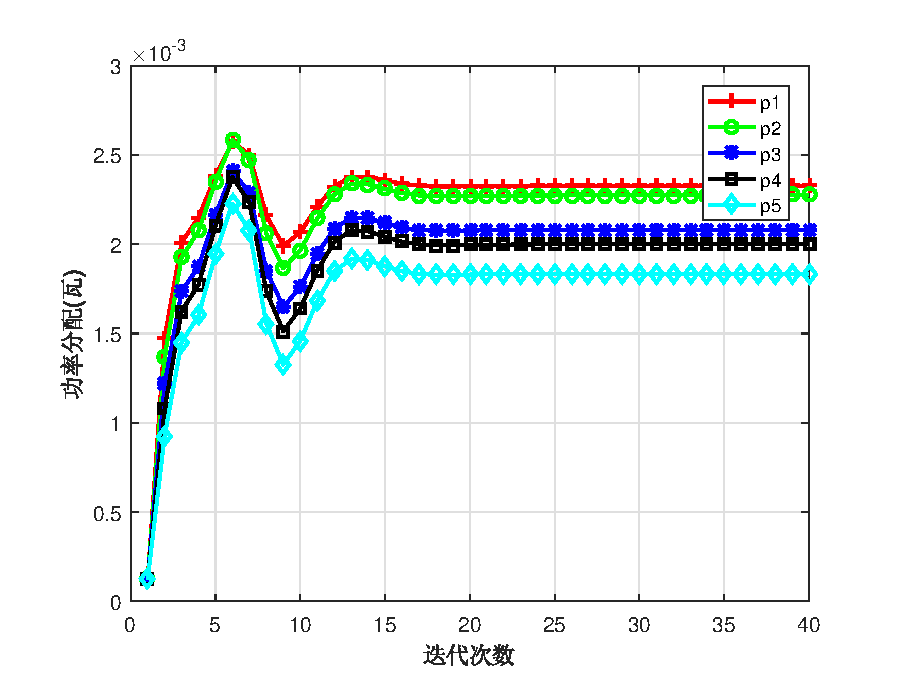
\includegraphics[width=10cm]{figures//chap3//pp.eps}
\caption{功率收敛性能}
\label{F2}
\end{figure}

图 \ref{F4} 显示了联合优化时系统总效用的收敛情况。从图中可以看出,网络系统总效用的收敛趋势与功率分配和计算率分配有关。观察到这一现象是合理的,因为方程 \eqref{E12} 给出了 $U$ 的定义。随着功率矢量 $\mathbf{p}$ 的增加,$R_i$ 也会对数增加,从而导致边际收益递减。因此,随着迭代次数的增加,效用值的增量会越来越小,最终导致效用值趋于稳定。当功率矢量$\mathbf{p}$ 和分子部分的执行效用$t_{i,exe}$ 随着计算功率矢量$\mathbf{f}$ 的增加而成反比减少时,$U$ 的分母会减少,分子会随着矢量$\mathbf{f}$ 的增加而增加。
\begin{figure}[H]
\centering
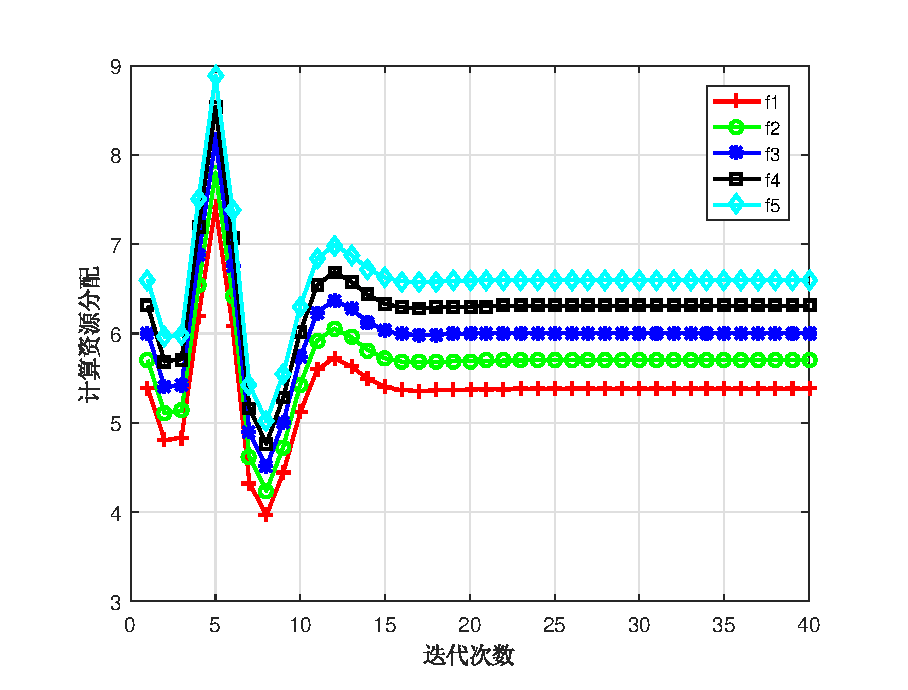
\includegraphics[width=10cm]{figures//chap3//ff.eps}
\caption{分配给RSU 的计算资源分配的收敛.}
\label{F3}
\end{figure}

\begin{figure}[H]
\centering
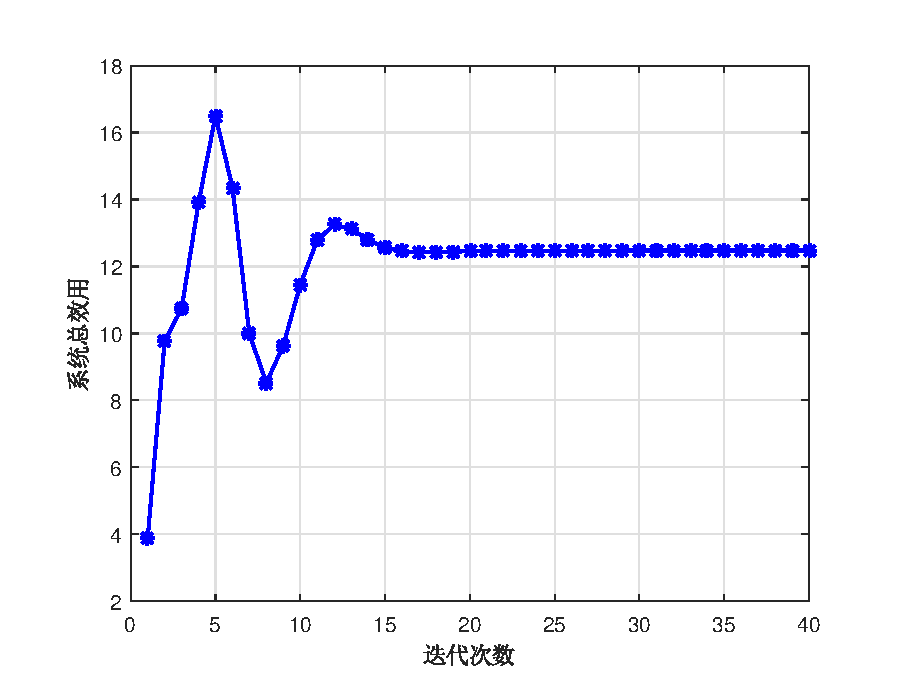
\includegraphics[width=10cm]{figures//chap3//ee.eps}
\caption{系统总效用的收敛.}
\label{F4}
\end{figure}

在支持 MEC 的车载云系统中,有必要考虑车辆的移动性。接下来,我们探讨了车辆移动对系统性能的影响。我们假设在指定时间段内车辆速度的任何变化都是微不足道的。为了进一步明确速度引起的多普勒频移对系统性能的影响,我们模拟了在系统中车辆速度恒定的条件下,基准值与增速测量值之间的比较。

图 \ref{F5} 展示了高流动性车辆环境下不同速度对系统性能的影响。
车辆环境下不同速度对系统性能的影响。由于 V2R 链路中的相对速度为零,且同一网络中所有车辆的速度相同,因此不存在多普勒效应。如图 \ref{F5} 所示,通信过程中的车速分别设置为20 m/s、30 m/s、40 m/s、50 m/s 和60 m/s。 因为车速越快,网络内的多普勒频移越大,这反过来又会导致信道不确定性增加,效用值随之下降。
\begin{figure}[H]
\centering
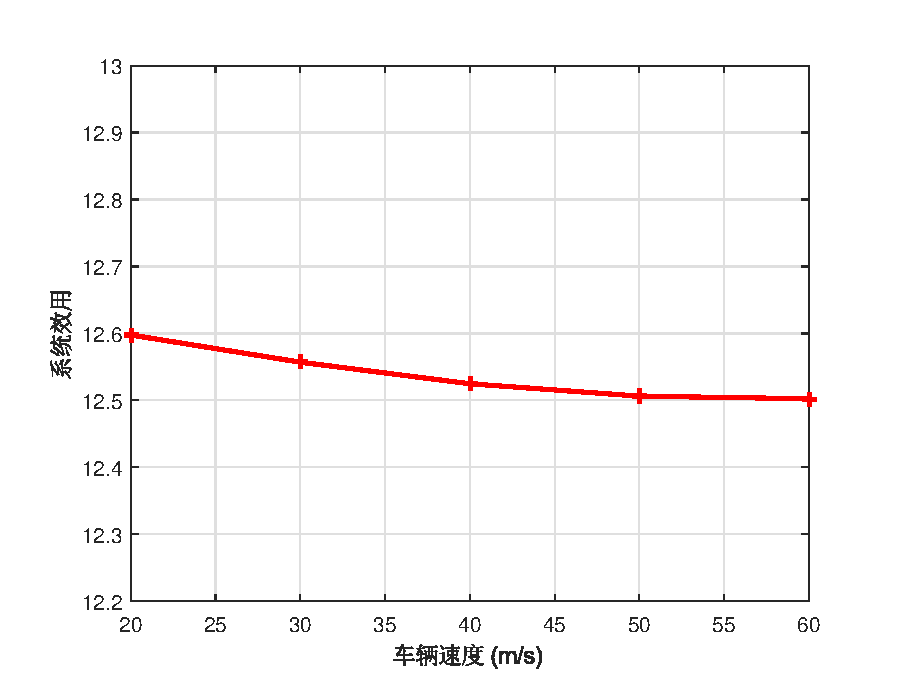
\includegraphics[width=10cm]{figures//chap3//diffspeed1.eps}
\caption{不同速度下系统总效用的对比.}
\label{F5}
\end{figure}

在考虑了车辆的流动性之后,进一步验证了所提方案的性能。图 \ref{F6} 显示了在使用不同的$\varepsilon_1$ 时,每辆车的相同速度和不同速度对总效用的影响。
\begin{figure}[H]
\centering
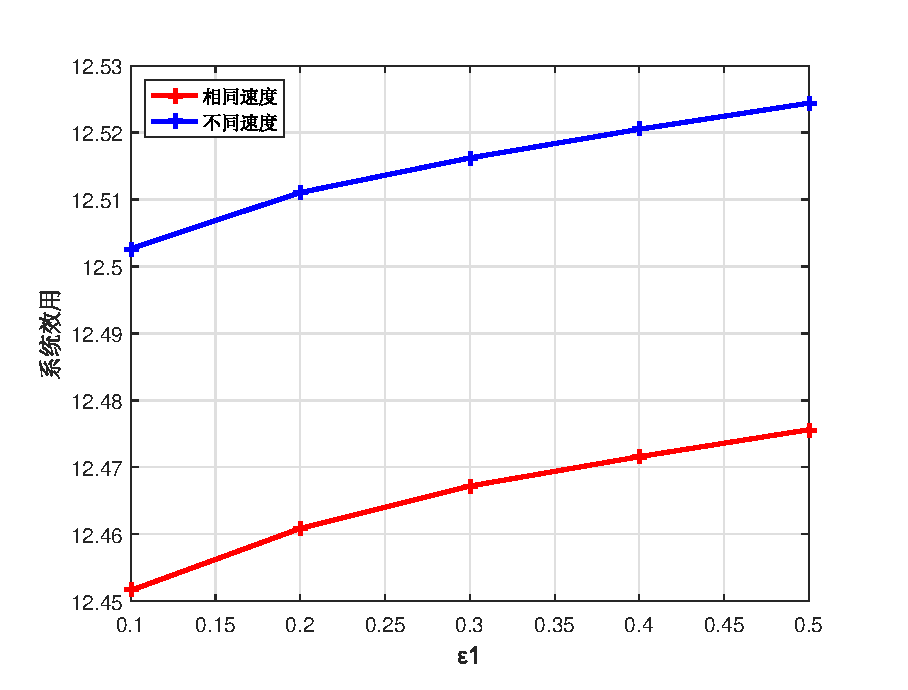
\includegraphics[width=10cm]{figures//chap3//diff_e1.eps}
\caption{不同 $\varepsilon_1$ 下系统总效用的变化.}
\label{F6}
\end{figure}

从图中可以看出,当 $\varepsilon_1$ 发生变化时,系统效用也会发生变化。每辆车在不同速度下的效用都高于所有车辆在相同速度下的效用。这一结果说明所提出的方法在复杂动态车辆网络中实施时具有很高的鲁棒性。

在计算率分配方面,我们选择默认的任务输入大小为 $d_u=420$KB (可参考 \cite{Xu2015})。它试图展示我们提出的算法的收敛性能。仿真结果表明,我们提出的方法优于三种基准方案。基准方案描述如下,
\begin{comment}
\begin{itemize}
\item[1)] 独立卸载和功率控制"(简称 "IOP"),即车辆独立执行功率控制和计算率分配,而不考虑彼此的最优值。
\item[2)] 在 " 无车辆功率控制"(简称 "Without-VPC")情况下,车辆的发射功率设定为卸载期间的平均功率。
\item[3)] 无计算速率分配"(表示为 "Without-CRA"),即在卸载过程中将云的计算速率分配设为固定值。
    %Similar to [?]Jiang2016  Similar to: \cite{Jiang2016},
\end{itemize}
\end{comment}

(1) 独立卸载和功率控制"(简称 "IOP"),即车辆独立执行功率控制和计算率分配,而不考虑彼此的最优值。

(2) 在 " 无车辆功率控制"(简称 "Without-VPC")情况下,车辆的发射功率设定为卸载期间的平均功率。

(3) 无计算速率分配"(表示为 "Without-CRA"),即在卸载过程中将云的计算速率分配设为固定值。

图 \ref{F7} 显示了不同情况下系统总效用的迭代收敛情况,图中显示鲁棒联合优化性能优于其他三种方案。从图中可以看出,四种方法在迭代后期都收敛到了一个稳定的值,其中建议方案的性能最好。

为了反映更真实的情况,每辆车所需的 CPU 任务负载(Megzcycles)往往不同,因此我们将五辆车的 CPU 任务负载(Megzcycles)分别设置为 1600、1700、1800、1900 和 2000。

\begin{figure}[H]
\centering
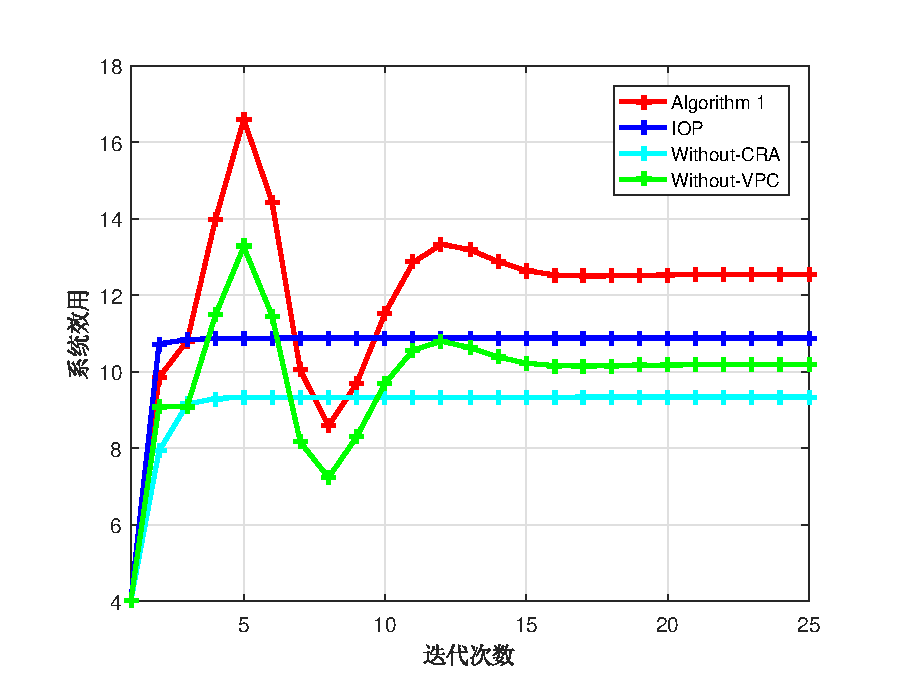
\includegraphics[width=10cm]{figures//chap3//compare.eps}
\caption{不同方案下系统总效用的收敛.}
\label{F7}
\end{figure}

从 \ref{F7} 可以看出,随着迭代次数的增加,车辆的平均系统效用逐渐发生变化并趋于稳定。在独立优化过程中,首先进行的是计算率分配,此时还不知道最优功率分配。采用功率和计算率交替优化的方法,每次迭代都能得到相应的最优值。单独优化首先优化功率向量 $\mathbf{p}$。 得到结果后,利用该结果优化计算率分配,然后优化计算率,得到系统。但是,如果采用联合优化,则两个变量都能达到最优值。

图 \ref{F8} 中绘制了不同任务输入大小 $d_u$ 时四种竞争方案的平均系统效用。图 \ref{F9} 显示了不同 $f_{total}$ 时的系统总成本比较。
\begin{figure}[H]
\centering
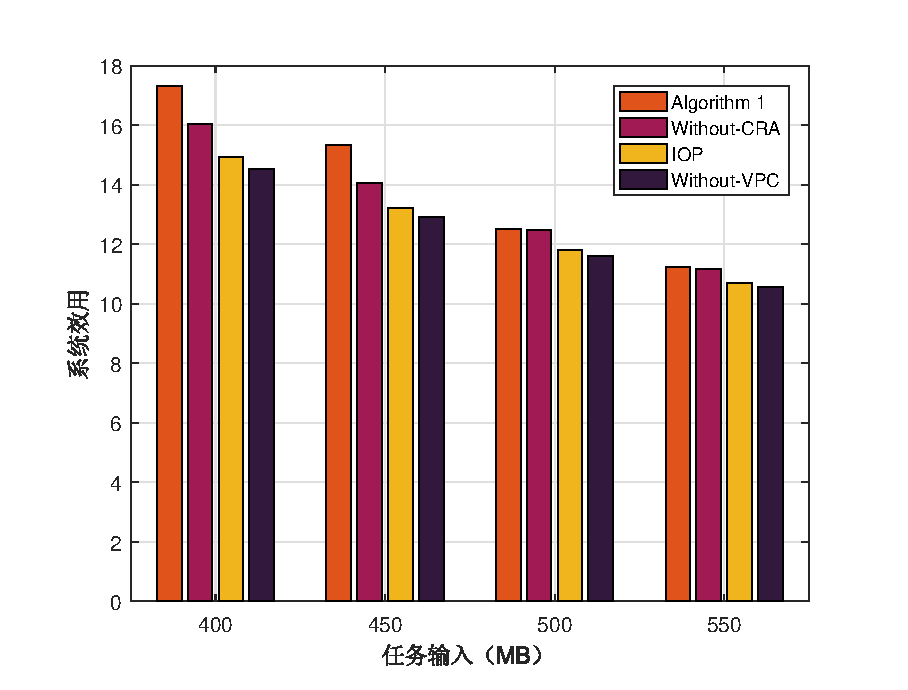
\includegraphics[width=10cm]{figures//chap3//diff_dup.eps}
\caption{不同输入数据 $d_u$ 下的系统效用.}
\label{F8}
\end{figure}
\begin{figure}[H]
\centering
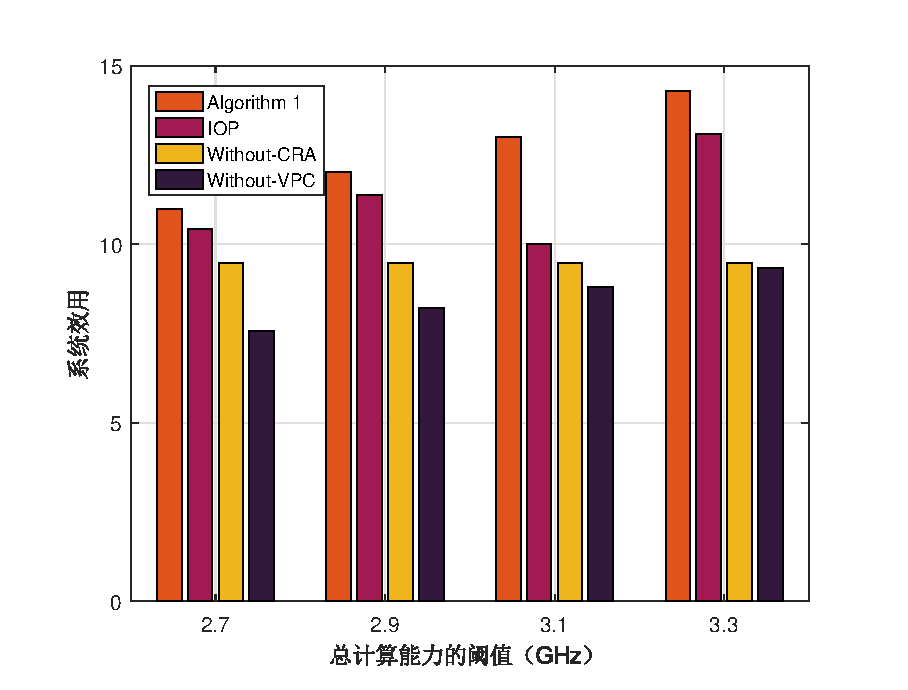
\includegraphics[width=10cm]{figures//chap3//diff_total.eps}
\caption{不同计算能力约束下的 $f_{total}$ 系统效用.}
\label{F9}
\end{figure}

从图 \ref{F8}中可以看出,所有方案的平均系统效用都随着任务输入量的增加而降低。图中还显示,其他方案的性能增益也有类似的趋势。
这一现象是合理的,因为根据 \eqref{E12} 中 $U$ 的定义,工作量的增加会对系统性能产生负面影响。
在图 \ref{F9}中,由于云的计算能力有限,当计算能力较小时,系统效用较小。
从图 \ref{F10} 中我们可以清楚地看到,当数据规模增大时,系统效用较小。当数据规模较大时,计算任务需要更多的上传时间。
\begin{figure}[H]
\centering
\includegraphics[width=10cm]{figures//chap3//diff_c.eps}
\caption{不同计算数据 $c_{i,e}$ 下的系统效用.}
\label{F10}
\end{figure}

\section{本章小结}\label{section3-5}
本章研究了车载网络中云辅助 MEC 的鲁棒功率控制和任务卸载的新方法。优化方案的目的是在最大化效用的同时保证车辆的 QoS。 由于信道存在不确定性,优化受到传输速率、计算通信延迟和同信道干扰概率形式的限制。最初的优化问题被表述为鲁棒性功率控制和任务卸载调度问题,很难解决。这里应用了 SCA 技术,将变量耦合的 NP 难问题转化为可处理的凸问题。鲁棒电源控制和任务卸载调度算法用于开发可行的解决方案。仿真结果表明,我们提出的算法得到了近似最优解。与现有方法相比,系统平均卸载效用得到显著改善。
\begin{comment}
\section{表格的引用}\label{section3-6}
表格的引用同样是使用\verb|\ref{}| 命令实现的。例如“表\verb|\ref{tab:ysubof}|” 输出的结果为:表\ref{tab:ysubof}。\LaTeX 会自动将其替换为表格的编号。例如:
\begin{verbatim}
燕山大学硕士学位论文参考文献规则的表格如表\ref{tab:ysubof} 所示。
\end{verbatim}
的效果如下:\\
燕山大学硕士学位论文参考文献规则的表格如表\ref{tab:ysubof} 所示。

\section{本章小结}\label{section3-7}
注意!从第二章开始应有`` 本章小结",主要总结本章所做的主要研究工作,研究成果等内容!!!

\end{comment}

%

% !Mode:: "TeX:UTF-8"
\chapter{无人机辅助的双向车道边缘计算网络的鲁棒功率控制方法与轨迹优化}

\label{chap:table}
\section{引言}\label{section4-1}
\label{chap:introduction}
在前一个章节中,主要研究了车联网的地面通信网络,然而随着城市化建设的加深,道路网络越来越复杂,车辆的地面通信网络容易受到建筑物的遮挡,同时地面基站也难以覆盖越来越多的通信车辆。因此本章研究了作为前沿通信技术的无人机作为空中基站辅助车联网通信,并着重考虑了更加实际的双向车道的场景。无人机具有灵活与高机动性的特性,可以更好地解决如今越来越复杂的通信网络。由于本文考虑的车辆环境均为高速移动场景,固定轨迹的无人机难以适应实时变化网络拓扑环境,因此实时优化无人机的飞行的航迹有助于提高辅助车辆通信的服务质量。此外,无人机飞行与作为空中基站时均为耗能设备,所以整个系统的能量效率也应备受关注。

综上所述,本章研究了一个双向车道下无人机辅助车辆网络能效最大化的场景,在这个网络中,车辆高速行驶于双向的高速公路上,地面基站位于道路的一侧,随着对向行驶的车辆的高速移动,向右行驶的车辆会逐渐驶出当前通信小区,无法与地面基站进行通信,此时,无人机可作为空中基站以接收车辆通信信号。无人机以固定的高度平行于道路进行无障碍飞行,我们提出的算法可以实时的判断当前时隙车辆如何选择通信对象使得系统的能量效率最大化。本章的贡献可以做出如下总结:首先,本章提出了一种无人机辅助双向车道场景下规划无人机航迹的系统模型,为了提高整个网络系统的能量效率,我们采用丁克尔巴赫方法与定价机制使得系统在最小的能耗下可以最大化总吞吐量,为了保证地面车辆用户的服务质量,在优化问题中建立了时变的车辆移动模型下的概率约束,尽可能地描述信道的不确定性。
\section{系统模型}\label{section4-2}
本章考虑了一个天地一体化网络,其中车辆行驶于双向的高速公路上,无人机从基站附近起飞,缓存基站提供的资源供道路上的车辆下载,因为是双向车道,基站位于坐标原点,高度为$h_0$,路边单元RSU的位置为$dd$,$D_R$代表了路边单元的覆盖范围的半径长度,
我们规定向右为正方向,定义车道索引$L=1$为车辆向右行驶,$L=-1$为向左行驶,由于基站位置固定,随者时间的推移,不可避免地存在一个方向的车辆会远离基站,势必影响其通过基站获取信息,此时,无人机向着基站的右方飞去,进而帮助远离基站的车辆获取需要的信息。
为了决策道路上的车辆需要从无人机还是基站获取信息,我们根据由一阶马尔可夫过程预测到车辆到基站的信道状态信息与车辆与空中基站无人机视距链路得到的信道状态信息分别得出车辆与两个数据中中心通信的信噪比,车辆会选择信噪比较大的一方请求资源,$x_m\left[t\right]=1$为车辆选择无人机进行通信,反之车辆选择基站进行通信。

在时隙$t$内,无人机的水平坐标为$q_U\left[t\right]=\left\{x_u\left[t\right],y_u\left[t\right]\right\}$
无人机在距离路面高度为$H$进行无障碍飞行,其飞行最大速度为$V_{max}$,车辆$M$的初始水平位置为$q_M\left[0\right]=\left\{x_0,y_0\right\}$,
假设车辆以速度$\nu_m$匀速直线行驶,根据之前定义的车道索引可以得出车辆$M$在第$t$时刻的水
平位置变化为$x_m\left[t\right]=x_0+l\nu_m t$,车辆$M$的水平位置 $q_M=\left\{x_m\left[n\right],y_0\right\}$
根据位置信息我们可以得到在第$t$时刻的距离信息
车辆$M$在$t$时隙与路边单元的距离为${{d}_{m,R}}\left[ t \right]=\left\| {{q}_{M}}\left[ t \right]-{{q}_{R}} \right\|=\sqrt{{{x}_{m}}{{\left[ t \right]}^{2}}+{{y}_{0}}^{2}+{{H}^{2}}}$
,车辆$M$在$t$时隙与无人机的距离为
$
{{d}_{m,U}}\left[ t \right]=\left\| {{q}_{M}}\left[ t \right]-{{q}_{U}}\left[ t \right] \right\|=\sqrt{{{\left( {{x}_{m}}\left[ t \right]-{{x}_{u}}\left[ t \right] \right)}^{2}}+{{\left( {{y}_{m}}\left[ t \right]-{{y}_{u}}\left[ t \right] \right)}^{2}}+{{H}^{2}}}\
$.系统模型如图\ref{systemuav}所示。
\begin{figure}[hptb!]
 \centering\small
 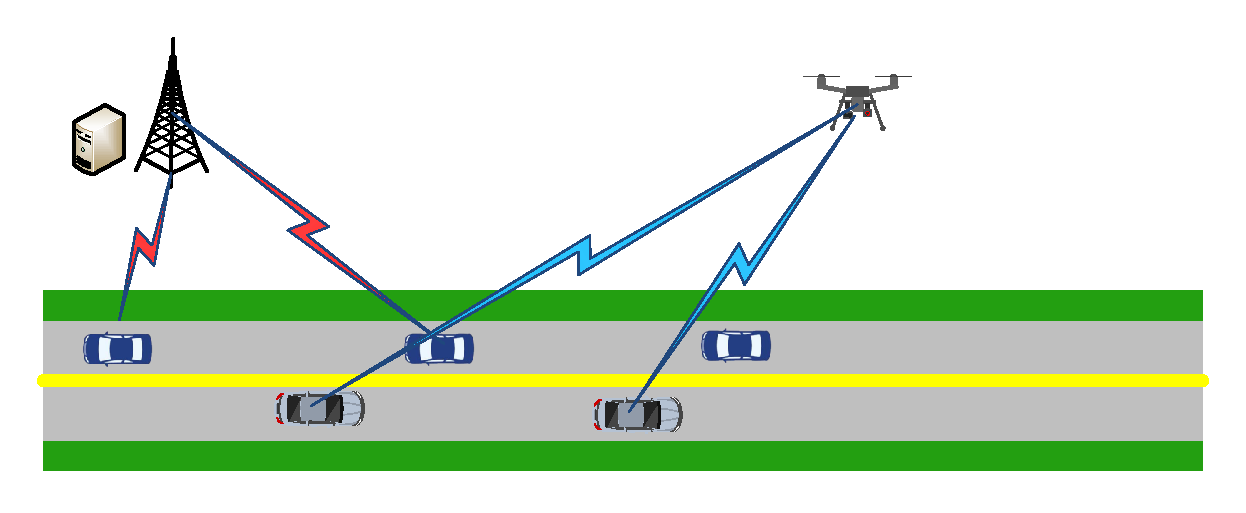
\includegraphics[width=0.6\textwidth]{systemuav}
 \Figcaption{无人机的系统模型}\label{systemuav}
\end{figure}

\subsection{车辆与地面基站通信计算与能耗模型}\label{section4-2-1}
由于车辆移动的快速性,对于车辆与路边单元的V2I通信,构建类似于前一章的一阶马尔可夫过程,在第$t$时刻的信道状态信息由前一时刻的状态预测得出,
即
\begin{equation} \label{E4-1}
%{\widetilde{g}}_{i,j}^k=L_{i,j}^2{\widetilde{h}}_{i,j}^2\xi_{i,j}^2
%h=\xi\tilde{h}+\sqrt{1-{{\xi }^{2}}}\zeta\    {\widetilde{g}}_{i,j}^k=L_{i,j}^2{\widetilde{h}}_{i,j}^2\xi_{i,j}^2
%{\widetilde{h}}_{m,R}=L_{m,R}^2{\widetilde{h}}_{m,R}^2\xi_{m,R}^2
h_{m}={\widetilde{h}}_{m}^2+{\hat{h}_{m}}^2,
\end{equation} \label{E4-2}
这里的${\widetilde{h}}_{m}$是一个观测值,${\hat{h}}_{m}$是一个服从参数为$a=\frac{1}{{L_{i,j}^k}^2({1-{\zeta_{i,j}^k}^2})}$的指数分布。
在第$t$个时隙,地面基站收到的第$m$辆车的信噪比(SNR)可以表示为:
\begin{equation}
\gamma_{m,R}\left[t\right]=\frac{p_m\left[t\right]h_{m,R}\left[t\right]}{\sigma^2}
\end{equation} \label{E4-3}
根据香农容量定理,车辆向地面基站的传输速率可以表示为:
\begin{equation}
R_{m,R}\left[t\right]=\log_2{\left(1+\gamma_{m,R}\left[t\right]\right)}
\end{equation}
车辆向地面基站传输的数据量可以表示为,
\begin{equation} \label{E4-4}
{{L}_{m,R}}={{B}_{0}}\underset{m=1}{\overset{M}{\mathop{\sum }}}\,\underset{t=1}{\overset{T}{\mathop{\sum }}}\,{{x}_{m}}\left[ t \right]R_{m,R}\left[t\right],
\end{equation}
其中$B_0$表示带宽,${{x}_{m}}\left[ t \right]=1$表示车辆当前时刻选择向地面基站传输数据,${{x}_{m}}\left[ t \right]=0$反之。


附属于路边单元的边缘服务器可以为收到的车辆数据进行数据计算处理
,因此计算卸载过程需要计算
资源,执行协作计算模型分裂的子任务。第$m$个车辆
的整个计算任务记为$A_m$,在某个时隙当其将任务分给路边单元时记为
$A_{R,m}={{z}_{m}}A_m$
我们定义$f_R$是路边单元的边缘服务器的CPU的加速频率,则计算时间可以表示为:
\begin{equation} \label{E4-4add}
t_{m}^{mec}=\frac{A_{R,m}}{f_R} \quad m \in \mathcal{M}.
\end{equation}
%同时我们使用瞬时的传输速率代替平均上传速率,由此可以得到车辆任务的上传时间为:、
%这里,我们将网络效用H(Am,i)定义为与访问子任务相关的卸载任务的计算满意度

车辆向地面基站路边单元通信时的传输能耗计算如下:
\begin{equation} \label{E4-5}
{{E}_{m,R}}=\underset{m=1}{\overset{M}{\mathop{\sum }}}\,\underset{t=1}{\overset{T}{\mathop{\sum }}}\,{{x}_{m}}\left[ t \right]{{p}_{m}}\left[ t \right]\
\end{equation}
\subsection{车辆与无人机通信与能耗模型}\label{section4-2-2}
对于车辆与无人机之间的通信中间没有障碍物遮挡,属于视距链路,构建了空中射频链路模型,
在第$t$个时隙,第$m$个车辆到无人机的信道增益为
\begin{equation} \label{E4-6}
h_{m,U}\left[t\right]=\frac{\varsigma_0}{{d_{m,U}\left[t\right]}^2}
\end{equation}
这里的$\varsigma_0$为单位距离1米下的功率增益,
%无人机与第$m$辆车之间的实时动态距离通过以下公式计算:
通过以上信息,无人机到车辆的传输速率为
\begin{equation} \label{E4-7}
R_{m,U}\left[t\right]=\log_2{\left(1+\gamma_{m,U}\left[t\right]\right)},
\end{equation}其中
\begin{equation} \label{E4-8}
\gamma_{m,U}\left[t\right]=\frac{p_m\left[t\right]h_{m,U}\left[t\right]}{\sigma^2},
\end{equation}表示车辆到无人机通信的信噪比,车辆向无人机空中基站传输的数据量可以表示为
\begin{equation} \label{E4-9}
%{{L}_{m,U}}={{B}_{0}}\underset{m=1}{\overset{M}{\mathop{\sum }}}\,\underset{t=1}{\overset{T}{\mathop{\sum }}}\,{{x}_{m}}\left[ t \right]{{\log }_{2}}\left( 1+{\gamma_{m,U}}\left[ t \right] \right)\
{{L}_{m,U}}={{B}_{0}}\underset{m=1}{\overset{M}{\mathop{\sum }}}\,\underset{t=1}{\overset{T}{\mathop{\sum }}}\,{{x}_{m}}R_{m,U}\left[t\right],
\end{equation}
其中$B_0$表示带宽,车辆向空中基站无人机通信时的传输能耗计算如下:
\begin{equation} \label{E4-10}
{{E}_{m,U}}=\underset{m=1}{\overset{M}{\mathop{\sum }}}\,\underset{t=1}{\overset{T}{\mathop{\sum }}}\,{{y}_{m}}\left[ t \right]{{p}_{m}}\left[ t \right]\
\end{equation}
由于无人机与路边单元之间具有良好的视距链路,因此我们认为车辆发送给无人机的数据
可以高效的传输到地面基站并由路边单元附属的边缘服务器进行数据处理。
\subsection{问题的定义}\label{section4-2-3}
在本节中,我们为无人机辅助的双向车道车辆制定了能效最大化问题。我们的目的是通过联合优化双向车道
上的车辆的发射功率以及无人机的轨迹来使得系统的总能效最大化.
首先,该网络通信系统的能效定义为
\begin{equation} \label{E4-11}
EE(\mathbf{P}, \mathbf{Q})=
{\frac{{{L}_{m}}\left( \mathbf{P}, \mathbf{Q} \right)}
{{{E}_{m}}\left( \mathbf{P} \right)}}
%EE(P,Q)=\sum\limits_{m=1}^{M}{\sum\limits_{n=1}^{N}{\frac{{{L}_{m,R}}\left[ n \right]+{{L}_{m,U}}\left[ n \right]}{{{E}_{m}}\left[ n \right]}}}
\end{equation}
式中的${{L}_{m}={L}_{m,R}+{L}_{m,U}}$是车辆向地面基站与空中基站发送的总的数据量,${E}_{m,R}$与${E}_{m,U}$分别是车辆与地面基站空中基站的能量消耗。
由于无人机飞行过程中会有能量的消耗,因此我们会更加关注车辆与无人机通信时的能耗问题,并考虑空中基站通信与地面基站通信的能量权衡,
因此系统的总功耗表示为${{E}_{m}=(1-\theta){L}_{m,R}+\theta{L}_{m,U}}$,其中$0\le \theta \le 1$是车辆与无人机通信时的能量成本的权重系数。
当$\theta$较大时意味着我们更加关注无人机的能耗成本。
最终的系统能效最大化问题如下表述:

\begin{align}
\max _{ \mathbf{P}, \mathbf{Q}, \mathbf{X} }  & EE(\mathbf{P}, \mathbf{Q}, \mathbf{X})                \label{E4-3end}\\
\text { s.t. }
& \Pr\left\{x_m\left[t\right]\gamma_{m,R}\left[t\right]+
y_m\left[t\right]\gamma_{m,U}\left[t\right]\geq \gamma_{th}\right\}\geq1-
\varepsilon_3, \forall m,t                                               \tag{\ref{E4-3end}{-1}}      \label{E4-3end1}\\  %信噪比中断概率约束
& 0\le p_m\left[t\right]\le p_{max}, \forall m                           \tag{\ref{E4-3end}{-2}}      \label{E4-3end2}\\  %功率阈值
& x_m\left[t\right] + y_m\left[t\right]=1, \forall m                     \tag{\ref{E4-3end}{-3}}      \label{E4-3end3}\\  %时隙分配加起来是一
& \frac{D_R}{\nu_m} \geq t_{m}^{mec}+t_{wired}                           \tag{\ref{E4-3end}{-4}}      \label{E4-3end4}\\  %这个是时隙的约束
& q_U^{n\mathrm{\ }+1}-q_U^{n\mathrm{\ }}\le tV_{max}, \forall m         \tag{\ref{E4-3end}{-5}}      \label{E4-3end5}    %无人机飞行轨迹
\end{align}

上式子中的\eqref{E4-3end1}表示了保证车辆通信的中断概率约束来保证服务质量,式子\eqref{E4-3end2}给出了
车辆最大最小发射功率的约束,式\eqref{E4-3end3}则代表了每个车辆每个时刻的任务只能向无人机或者地面基站
进行卸载,
 $\gamma_{th}$是信噪比的阈值为一个固定值,\eqref{E4-3end4}表示了需要调度车辆在其驶出路边单元覆盖范围
之前服务器要完成完成数据的计算,其中$t_{wired}$是路边单元向边缘服务器发送数据时的
固定时间。无人机的飞行轨迹受到\eqref{E4-3end5}的约束,


\section{能效最大化问题求解}\label{section4-3}
在本节中,上一章节的能效最大化问题会分解为两个子问题进行求解。对于难以求解的分式规划,可以使用丁克尔巴赫方法
将其转化为易于求解的减式规划进行求解。首先固定车辆的发射功率后求解无人机的飞行轨迹,然后固定无人机的飞行轨迹再求解
车辆的发射功率,如此进行交替迭代优化,直至算法收敛。注意到前一节中问题\eqref{E4-3end}是一个非凸的问题,我们提出了
一种联合功率分配与无人机轨迹规划的方案来有效地处理这个问题,
将问题\eqref{E4-3end}解耦成两个子问题。
\subsection{概率约束的近似与车辆发射功率优化问题}\label{section4-3-1}
在前一节的式\eqref{E4-3end1}中我们发现车辆的功率功率在概率约束中存在较为复杂的耦合关系,是难以直接求解的,
针对这种情况,我们将采用积分变换的方式将复杂的概率约束问题转化为较为简单的形式。

定理:对于\eqref{E4-3end1},车辆用户的中断概率约束
\begin{align}
\Pr\left\{x_m\left[t\right]\gamma_{m,R}\left[t\right]+y_m\left[t\right]\gamma_{m,U}\left[t\right] \geq \gamma_{th}\right\}\geq1-\varepsilon_3    \notag
\end{align}
等价于:
\begin{equation} \label{E4-13}
\begin{gathered}
p_m\left[t\right]x_m\left[t\right]\ln \left(1-a \varepsilon_3\right)+(\gamma_{th}-y_m\left[t\right]\gamma_{m,U})\left[t\right] a \sigma^2
\leq a p_m\left[t\right]x_m\left[t\right]\hat{h}_{m}\left[t\right]
\end{gathered}
\end{equation}
%\textcolor[RGB]{202,12,22}{巴拉巴拉}

证明:
\begin{align} \label{E4-14}
\frac{x_m\left[t\right]p_m\left[t\right]h_{m,R}\left[t\right]}{\sigma^2}\geq \gamma_{th}-y_m\left[t\right]\gamma_{m,U}\left[t\right] \\
\Leftrightarrow
p_m\left[t\right]{\widetilde{h}}_{m}\left[t\right]\geq \frac{{(\gamma_{th}-y_m\left[t\right]\gamma_{m,U}\left[t\right])\sigma^2}}{x_m\left[t\right]}
-p_m\left[t\right]{\hat{h}}_{m}\left[t\right]   \notag
\end{align}
%$\frac{{(SNR_{th}-y_m\left[t\right]\gamma_{m,U})\sigma^2}}{x_m\left[t\right]}$
因此车辆用户的中断概率约束做出重新表述如下:
\begin{align} \label{E4-15}
\Pr\left\{x_m\left[t\right]\gamma_{m,R}\left[t\right]+y_m\left[t\right]\gamma_{m,U}\left[t\right] \geq \gamma_{th}\right\}\geq1-\varepsilon_3    \\
\Leftrightarrow
\Pr\left\{{\widetilde{h}}_{m}\left[t\right]\geq \frac{{(\gamma_{th}-y_m\left[t\right]\gamma_{m,U}\left[t\right])\sigma^2}}{p_m\left[t\right]x_m\left[t\right]}
-{\hat{h}}_{m}\left[t\right]\right\}\geq1-\varepsilon_3                          \notag
\end{align}
由于随机变量$\widetilde{h}$的概率密度函数为$f_x={{e}^{-ax}}$,通过积分变换可得:
\begin{align} \label{E4-16}
&\int_{0}^{\frac{{(\gamma_{th}-y_m\left[t\right]\gamma_{m,U})\sigma^2}}{p_m\left[t\right]x_m\left[t\right]}
-{\hat{h}}_{m}\left[t\right]}{e^{-ax}dx}\le \varepsilon_3 \\
\Leftrightarrow
&p_m\left[t\right]x_m\left[t\right]\ln \left(1-a \varepsilon_3\right)+(\gamma_{th}-y_m\left[t\right]\gamma_{m,U}\left[t\right]) a \sigma^2
\leq a p_m\left[t\right]x_m\left[t\right]\hat{h}_{m}\left[t\right]   \notag
%GVRR.* P_m.*X' >= SNRth*Delta+ GVUU.*P_m.*Y'+log(1-e1)*P_m.*X'
\end{align}
为了表达方便,我们定义$\gamma_{m,U}\left[t\right]=p_m\left[t\right]\eta_{m,U}\left[t\right]$,其中$\eta_{m,U}\left[t\right]=h_{m,U}\left[t\right]/{\sigma^2}$,
将式子\eqref{E4-16}改写为:
\begin{equation} \label{E4-17}
p_m\left[t\right]x_m\left[t\right]\ln \left(1-a \varepsilon_3\right)+(\gamma_{th}-y_m\left[t\right]p_m\left[t\right]\eta_{m,U}\left[t\right]) a \sigma^2
\leq a p_m\left[t\right]x_m\left[t\right]\hat{h}_{m}\left[t\right]
\end{equation}

在求解车辆发射功率的过程中,需要每个时隙都要进行功
率分配与无人机轨迹规划并进行多次迭代,
关于车辆发射功率$p_m\left[t\right]$的子问题如下描述:
\begin{align} 
\max _{ \mathbf{P}} &   ={\frac{{{L}_{m}}\left( \mathbf{P} \right)}
{(1-\theta){E}_{m,R}\left( \mathbf{P} \right)+\theta{E}_{m,R}\left( \mathbf{P} \right)}}         \label{E4-4end}\\
\text { s.t. }
& \eqref{E4-3end1},\eqref{E4-3end4}                                 \tag{\ref{E4-4end}{-1}}      \label{E4-4end1}
\end{align}
注意到问题\eqref{E4-4end}是一个分式规划问题,
为了将其转化为减式规划问题,拟采用丁克尔巴赫方法求解。
\begin{align} \notag
F(\chi)= & \max _{ \mathbf{P}} \sum_{t=1}^T \sum_{m=1}^M {B}_{0}x_{m}^{\left\{ l \right\}}\left[ t \right] %x_m\left[t\right]
\log_2{\left(1+p_m\left[t\right]\eta_{m,R}^{\left\{ l \right\}}\left[t\right]\right)}                         \\       \label{E4-5end}
& + \sum_{t=1}^T \sum_{m=1}^M {B}_{0}x_{m}^{\left\{ l \right\}}\left[ t \right]
\log_2{\left(1+p_m\left[t\right]\eta_{m,U}^{\left\{ l \right\}}\left[t\right]\right)}                         \\ \notag
& -\chi \sum_{t=1}^T \sum_{m=1}^M{(1-\theta)x_{m}^{\left\{ l \right\}}\left[ t \right]p_m\left[t\right]
+\theta y_{m}^{\left\{ l \right\}}\left[ t \right]p_m\left[t\right]}                                          \\ \notag
\text { s.t. }
& \eqref{E4-3end1},\eqref{E4-3end4}                                       \tag{\ref{E4-5end}{-1}}                      \label{E4-5end1}
\end{align}

上式中的$\eta_{m,R}^{\left\{ l \right\}}\left[t\right]=h_{m,R}\left[t\right]/{\sigma^2}$,
$\eta_{m,U}^{\left\{ l \right\}}\left[t\right]=h_{m,U}\left[t\right]/{\sigma^2}$
在每$l$次迭代时视为常数,对于凸问题\eqref{E4-5end},
我们可以构建拉格朗日函数并运用拉格朗日对偶法进行求解:
\begin{align}\label{E4-20}
&L\left(\mathbf{p},\lambda\right)\\
&=\sum_{t=1}^T \sum_{m=1}^M {B}_{0}x_{m}^{\left\{ l \right\}}\left[ t \right] %x_m\left[t\right]
\log_2{\left(1+p_m\left[t\right]\eta_{m,R}^{\left\{ l \right\}}\left[t\right]\right)}+                                                      \notag
\sum_{t=1}^T \sum_{m=1}^M {B}_{0}y_{m}^{\left\{ l \right\}}\left[ t \right]
\log_2{\left(1+p_m\left[t\right]\eta_{m,U}^{\left\{ l \right\}}\left[t\right]\right)}                     \\                                \notag
&-\chi \sum_{t=1}^T \sum_{m=1}^M{(1-\theta)x_{m}^{\left\{ l \right\}}\left[ t \right]p_m\left[t\right]
+\theta y_{m}^{\left\{ l \right\}}\left[ t \right]p_m\left[t\right]} \\
&-\sum\limits_{t=1}^{T}{\sum\limits_{m=1}^{M}{{{\lambda }_{m,t}}}}\left( ({{\gamma }_{th}}-{{y}_{m}}\left[ t \right]{{p}_{m}}\left[ t \right]{{\eta }_{m,U}}\left[ t \right])a{{\sigma }^{2}}-a{{p}_{m}}\left[ t \right]{{x}_{m}}\left[ t \right]{{{\hat{h}}}_{m}}\left[ t \right]+{{p}_{m}}\left[ t \right]{{x}_{m}}\left[ t \right]\ln \left( 1-a{{\varepsilon }_{3}} \right) \right)                                                                 \notag
%&-\sum_{t=1}^T\sum_{m=1}^M\lambda_{m,t}\Big[  (\gamma_{th}-y_m\left[t\right]p_m\left[t\right]\eta_{m,U}\left[t\right]) a \sigma^2 \\
%&-a p_m\left[t\right]x_m\left[t\right]\hat{h}_{m}\left[t\right]+ p_m\left[t\right]x_m\left[t\right]\ln \left(1-a \varepsilon_3\right)\Big]  \notag,
\end{align}
其中的拉格朗日乘子$\lambda_{m,t}\geq 0$,则\eqref{E4-20}的拉格朗日对偶函数表示为:
\begin{equation} \label{E4-21}
D(\mathbf{\lambda})=\max _{\substack{0 \leq P_m[t] \leq P_{\max }}} L\left(\mathbf{p_m},\mathbf{\lambda}\right)
\end{equation}
其中\eqref{E4-21}的对偶问题为:
\begin{equation} \label{E4-22}
\min_{\substack{\lambda_{m,t}\geq 0}} D\left(\mathbf{p_m},\mathbf{\lambda}\right)
\end{equation}
问题\eqref{E4-22}是一个凸问题且满足Karush-Kuhn-Tucker(KKT)条件,
在使用KKT条件的类似求解过程中可令其一阶导数为等于零:
\begin{align}\label{E22add}
\frac{\partial D\left(\mathbf{p_m},\lambda,\mu\right)}{\partial p_i}=A_i-\Bigl[\sum_{j=1,j\neq i}^{M}\left(A_j\frac{{\bar{\gamma}}_j\left(e^{\widetilde{p}}\right){\bar{G}}_{k,j}}{e^{{\widetilde{p}}_j}{\bar{G}}_{j,j}}\right)\\
+\lambda_i\mathrm{\Pi}_ie^{-{\widetilde{p}}_i}+\mu_i{\hat{g}}_{i,j}^k\Bigl]e^{{\widetilde{p}}_i}=0\notag,
\end{align}
\textcolor[RGB]{202,12,22}{再加点橙子梯度}
\subsection{无人机飞行轨迹规划问题}\label{section4-3-2}
%\textcolor[RGB]{202,12,22}{ }
通过前一节求得车辆功率的分配时,对于无人机轨迹的优化问题可以如下求解:
当每次迭代的车辆发射功率$\left\{ {{P_m}^{\left\{ l \right\}}} \right\}$和时隙分配
%无人机的轨迹$\left\{ {{Q}^{\left\{ l \right\}}} \right\}$
给定后,关于无人机的轨迹的优化描述如下:
\begin{align} \label{E4-23}
\max _{ \mathbf{Q}} &   ={\frac{{{L}_{m,R}+{{L}_{m,U}}\left( \mathbf{Q} \right)}}
{(1-\theta){{E}_{\text{t}}}^{R,\left\{ l \right\}}+\theta{{E}_{\text{t}}}^{U,\left\{ l \right\}}}}        \\
\text { s.t. }
& \eqref{E4-3end2}                                                       \tag{\ref{E4-23}{-1}}           \label{E4-23-1}
\end{align}
其中,
\begin{equation} \label{E4-24}
{{L}_{m,U}}\left( \mathbf{Q} \right)={{\log }_{2}}\left( 1+\frac{\varphi _{m,U}^{\{l\}}\left[ t \right]}{\left\| {{q}_{M}}\left[ t \right]-{{q}_{U}}\left[ t \right] \right\|+{{H}^{2}}} \right)\
\end{equation}
这里的${\varphi _{m,U}^{\{l\}}\left[ t \right]}=\frac{p_{_{m}}^{\{l\}}\left[ t \right]\varsigma_0}{\sigma^2}$,
我们注意到问题\eqref{E4-23}目标函数的分子部分是非凹问题,拟采用连续凸逼近方法对目标函数进行近似。在
${{q}^{\left\{ l \right\}}}\left[t\right]$
的局部点处,对式\eqref{E4-23}的分子部分的对数形式进行一阶泰勒展开,过程如下:
\begin{align} \label{E4-25}
&{{\log }_{2}}\left( 1+\frac{\varphi _{m,U}^{\{l\}}\left[ t \right]}{\left\| {{q}_{M}}\left[ t \right]-{{q}_{U}}\left[ t \right] \right\|+{{H}^{2}}} \right)\ \\    \notag
&\geq\left(\omega _{_{m}}^{\{l\}}\left[ t \right] {{\left\| {{q}_{M}}\left[ t \right]-{{q}_{U}}\left[ t \right] \right\|}^{2}}-{{\left\| {{q}_{M}}\left[ t \right]-q_{U}^{\{l\}}\left[ t \right] \right\|}^{2}}+\rho _{m}^{\{l\}}\left[ t \right] \right) \\  \notag
&\triangleq R_{m,U}^{\{l\}}(\mathbf{q}[t])  \notag
\end{align}
其中,
\begin{align} \label{E4-26}
\omega _{_{m}}^{\{l\}}\left[ t \right]=\frac{-\varphi _{m,U}^{\{l\}}\left[ t \right]}{\ln 2\left( {{\left\| {{q}_{M}}\left[ t \right]-q_{U}^{\{l\}}\left[ t \right] \right\|}^{2}}+{{H}^{2}} \right)}\cdot \frac{1}{{{\left\| {{q}_{M}}\left[ t \right]-q_{U}^{\{l\}}\left[ t \right] \right\|}^{2}}+{{H}^{2}}+\varphi _{m,U}^{\{l\}}\left[ t \right]}
\end{align}
并且,
\begin{equation} \label{E4-27}
\rho_{_{m}}^{\{l\}}\left[ t \right]={{\log }_{2}}\left( 1+\frac{\varphi _{m,U}^{\{l\}}\left[ t \right]}{\left\| {{q}_{M}}\left[ t \right]-q_{U}^{\{l\}}\left[ t \right] \right\|+{{H}^{2}}} \right)\
\end{equation}
问题\eqref{E4-23}进一步转化为:
\begin{align} \label{E4-29}
\max _{ \mathbf{Q}}  &  ={\frac{{{L}_{m,R}+\sum\limits_{t=1}^{T}{\sum\limits_{m=1}^{M}{{{B}_{0}}}}y_{m}^{\left\{ l \right\}}\left[ t \right]R_{m,U}^{\{l\}}(\mathbf{q}[t])}}
{(1-\theta){{E}_{\text{t}}}^{R,\left\{ l \right\}}+\theta{{E}_{\text{t}}}^{U,\left\{ l \right\}}}}       \\
\text { s.t. }
& \eqref{E4-3end2}                                                       \tag{\ref{E4-29}{-1}}           \label{E4-29-1}
\end{align}
至此,问题\eqref{E4-23}的非凸问题部分转化成了凸的可解的形式,可以使用凸优化工具箱CVX求解。
\subsection{计算时间约束转化与时隙资源分配问题}\label{section4-3-3}
由不等式\eqref{E4-3end4}与$A_{R,m}={{z}_{m}}A_m$,我们得知时隙的分配受到服务器计算时间的制约,
因此可以很容易得到:
\begin{equation} \label{E4-30}
{{z}_{m}}=\underset{t=1}{\overset{T}{\mathop{\sum }}}{{x}_{m}}\left[ t \right]   ,\qquad\forall \!\!\!\!\!\! \quad m \in \mathcal{M}
\end{equation}
即车辆向地面基站通信的所有的时隙加起来要小于
车辆在基站的覆盖范围内。当功率 和轨迹 {}给定时,关于分配时隙的子问题如下:
\begin{align} \label{E4-31}
\max _{ \mathbf{X},\mathbf{Y}}  &  ={\frac{{{L}_{m,R}\left( \mathbf{X} \right)+{{L}_{m,U}}\left( \mathbf{Y} \right)}}
{(1-\theta){{E}_{\text{t}}}^{R,\left\{ l \right\}}\left( \mathbf{X} \right)+\theta{{E}_{\text{t}}}^{U,\left\{ l \right\}}\left( \mathbf{Y} \right)}}     \\
\text { s.t. }
& \eqref{E4-3end3},\eqref{E4-3end4}                                                        \tag{\ref{E4-31}{-1}}           \label{E4-31-1}
\end{align}
这是一个分式规划的问题,我们可以使用与问题\eqref{E4-4end}类似的丁克尔巴赫方法将原问题转化为、
易于求解的减式规划,即式子\eqref{E4-31}等价于一个可以使用凸优化工具箱(CVX)迭代求解的线性规划问题。
%\textcolor[RGB]{202,12,22}{与(3-17)类似,(3-31)中的分数形式的目标函数可以通过丁克尔巴赫方法转换为减法形式,因此可以通过使用凸优化工具包(例如CVX[51]) 迭代解决。}


\begin{comment}  %这个也可以使用,就是字体有点粗
\begin{table}[htbp!]
 \centering\small
 \renewcommand\arraystretch{1.5}   %latex三线表中各行间隔
 %\Tablecaption{系统仿真参数}\label{biao42}
\begin{tabular*}{\hsize}{@{\extracolsep{\fill}}l l l l}
 \toprule
 算法4-3基于固定节点功率分配的无人机轨迹优化方案           \\
 \midrule
    Step1:开始。                                      \\
    Step2:输入功率矩阵$P$和车辆分簇信息$C$            \\
   Step3:地面基站高度面基站高度面基站高度面基站高度  \\
    Step4:计算无人机轨迹                              \\
    Step5:地面基站高度面基站高度面基站高度面基站高度  \\
    Step6:执行$l=l+1$                         \\
   Step7:重复执行Step3至Step5,直到满足收敛条件      \\
    Step8:结束。                         \\
 \bottomrule
 \end{tabular*}
\end{table}
\end{comment}

%\subsection{计算资源分配}\label{section4-3-4}
%\section{联合资源分配方案}\label{section4-4}
%\subsection{概率约束转化}\label{section4-4-1}
%\subsection{功率分配}\label{section4-4-2}

\section{算法与仿真验证}\label{section4-5}

\subsection{总体算法设计}\label{section4-5-1}
原始的问题\eqref{E4-3end}被分为三个子问题,它们已在上述小节中分别得到解决。然后使用交替迭代的方法
\begin{comment}
\begin{table}[htbp!]
 \centering\small
% \Tablecaption{}\label{biao4-1}
\begin{tabular*}{\hsize}{@{\extracolsep{\fill}}c c c c}
 \toprule
 &&基于固定节点功率分配的无人机轨迹优化方案                   \\
 \midrule
 &&Step1:开始。                \\
 &&Step2:输入功率矩阵$P$和车辆分簇信息$C$               \\
 &&Step2:地面基站高度面基站高度面基站高度面基站高度                         \\
 \bottomrule
 \end{tabular*}
\end{table}

\begin{tabular}{lcr}
    \toprule
    Item  &amp; Quantity &amp; Price (\$) \\
    \midrule
    Apple &amp; 2        &amp; 1.50       \\
    Banana &amp; 3       &amp; 1.00       \\
    Cherry &amp; 5       &amp; 0.50       \\
    \bottomrule
\end{tabular}
\end{comment}


\begin{tabular*}{\hsize}{@{\extracolsep{\fill}}l l l l}
%\begin{tabular}{lcr}
    \toprule
    算法4-3基于固定节点功率分配的无人机轨迹优化方案           \\
    \midrule
    Step1:开始。                                      \\
    Step2:输入功率矩阵$P$和车辆分簇信息$C$            \\
    Step3:地面基站高度面基站高度面基站高度面基站高度  \\
    Step4:计算无人机轨迹                              \\
    Step5:地面基站高度面基站高度面基站高度面基站高度  \\
    Step6:执行$l=l+1$                         \\
   Step7:重复执行Step3至Step5,直到满足收敛条件      \\
    Step8:结束。                         \\
    \bottomrule
\end{tabular*}

\subsection{仿真分析}\label{section4-5-2}
在本小节中,为了检验算法的有效性并评估其性能,我们提供了数值仿真结果,主要评估了联合优化无人机轨迹和信道功率分配方案(J-TOPA)的性能,并介绍了
无人机固定位置悬浮方案与固定无人机轨迹的方式两种方案,并且将我们的方案与之对比。
悬浮方案中无人机在固定位置上方悬停以简化计算复杂度,其中我们模拟的双向车道长度为800米,宽度为30米,除非特别说明
道路上选取6辆车进行仿真,其中每辆车以不同的速度匀速直线行驶。仿真中的主要参数见表\ref{biao4-1}:

\begin{table}[htbp!]
 \centering\small
 \renewcommand\arraystretch{1.5}   %latex三线表中各行间隔
 \Tablecaption{系统仿真参数}\label{biao4-1}
\begin{tabular*}{\hsize}{@{\extracolsep{\fill}}c c c c}
 \toprule
    \qquad\qquad 符号         &\qquad\qquad 参数                       & \qquad\qquad 数值            \\
 \midrule
    \qquad\qquad $H$          &\qquad\qquad 无人机的飞行高度           & \qquad\qquad 100             \\
    \qquad\qquad $T$          &\qquad\qquad 时隙个数                   & \qquad\qquad 70              \\
    \qquad\qquad $h$          &\qquad\qquad 地面基站高度               & \qquad\qquad 5               \\
    \qquad\qquad $V_{max}$    &\qquad\qquad 每个时隙无人机最大飞行距离 & \qquad\qquad 2.5m            \\
    \qquad\qquad $\sigma^2$   &\qquad\qquad 噪声方差                   & \qquad\qquad 5               \\
    \qquad\qquad $\gamma_{th}$&\qquad\qquad 信噪比阈值                 & \qquad\qquad 96dBm           \\
    \qquad\qquad $\varsigma_0$&\qquad\qquad 路径损耗指数               & \qquad\qquad 4               \\
 \bottomrule
 \end{tabular*}
\end{table}



\section{本章小结}\label{section4-6}

表格的引用同样是使用\verb|\ref{}| 命令实现的。例如“表\verb|\ref{tab:ysubof}|” 输出的结果为:表\ref{biao4-1}。\LaTeX 会自动将其替换为表格的编号。例如:
4
的效果如下:\\
注意!从第二章开始应有``本章小结",主要总结本章所做的主要研究工作,研究成果等内容!!!


燕山大学硕士学位论文参考文献规则的表格如表\ref{biao4-1}所示。
%\section{本章小结}\label{section4-7}
\begin{table}[h] %h表示三线表在当前位置插入
\setlength{\abovecaptionskip}{0.05cm} %设置三线表标题与第一条线间距
\centering\small
\caption{{系统仿真参数}}
%\caption{\textbf{The characteristics of various methods}}
%表头文本加黑,但不加黑Table 1.字样,引入包即可:\usepackage[labelfont=bf]{caption}
%\arrayrulecolor{black} %设置三线表线条颜色:黑色
\begin{tabular*}{\hsize}{@{\extracolsep{\fill}}c c c c} %{\hsize}使三线表自适应宽度,c表示文本居中
  \hline
  参数 & 数值 \\
  \hline
  人机高度  & 100 \\
  1地面基站高度 & 222  \\
  地面基站高度面基站高度面基站高度面基站高度  & 2222  \\
  \hline
\end{tabular*}
\end{table}

\begin{comment}
\begin{table}[h] %h表示三线表在当前位置插入
\setlength{\abovecaptionskip}{0.05cm} %设置三线表标题与第一条线间距
\centering\small
\caption{{系统仿真参数}}
%\caption{\textbf{The characteristics of various methods}}
%表头文本加黑,但不加黑Table 1.字样,引入包即可:\usepackage[labelfont=bf]{caption}
%\arrayrulecolor{black} %设置三线表线条颜色:黑色
\begin{tabular*}{\hsize}{@{\extracolsep{\fill}}c c c c} %{\hsize}使三线表自适应宽度,c表示文本居中
  \hline
  参数 & 数值 \\
  \hline
  人机高度  & 100 \\
  1地面基站高度 & 222  \\
  地面基站高度面基站高度面基站高度面基站高度  & 2222  \\
  \hline
\end{tabular*}
\end{table}
\end{comment}

\begin{comment}
\begin{equation}
\begin{aligned}
\max _{ \boldsymbol{P}, \boldsymbol{Q}} & EE(\boldsymbol{P},\boldsymbol{Q}) \\
\text { s.t. }
& Pr\left\{x_m\left[t\right]SNR_{m,R}\left[t\right]+y_m\left[t\right]SNR_{m,U}\left[t\right]\geq S N R_{th}\right\}\geq1-\varepsilon_1, \forall m,t \\
& q_U^{n\mathrm{\ }+1}-q_U^{n\mathrm{\ }}\le tV_{max}, \forall m \\
& x_m\left[t\right] + y_m\left[t\right]=1, \forall m\\
& 0\le p_m\left[t\right]\le p_{max}, \forall m
\end{aligned}
\end{equation}

\begin{eqnarray}
\begin{aligned}
\max _{ \boldsymbol{P}, \boldsymbol{Q}} & EE(\boldsymbol{P},\boldsymbol{Q}) \label{equ-s1a}\\
\text { s.t. }
& Pr\left\{x_m\left[t\right]SNR_{m,R}\left[t\right]+y_m\left[t\right]SNR_{m,U}\left[t\right]\geq S N R_{th}\right\}\geq1-\varepsilon_1, \forall m,t  \label{equ-s2a}\\
& q_U^{n\mathrm{\ }+1}-q_U^{n\mathrm{\ }}\le tV_{max}, \forall m  \label{equ-s3a}\\
& x_m\left[t\right] + y_m\left[t\right]=1, \forall m \label{equ-s4a}\\
& 0\le p_m\left[t\right]\le p_{max}, \forall m  \label{equ-v1a}
\end{aligned}
\end{eqnarray}

\begin{align}
\max _{ \boldsymbol{P}, \boldsymbol{Q}} & EE(\boldsymbol{P},\boldsymbol{Q}) \label{equ-s1a}\\
\text { s.t. }
& Pr\left\{x_m\left[t\right]SNR_{m,R}\left[t\right]+y_m\left[t\right]SNR_{m,U}\left[t\right]\geq S N R_{th}\right\}\geq1-\varepsilon_1, \forall m,t  \label{equ-s2a}\\
& q_U^{n\mathrm{\ }+1}-q_U^{n\mathrm{\ }}\le tV_{max}, \forall m  \label{equ-s3a}\\
& x_m\left[t\right] + y_m\left[t\right]=1, \forall m \label{equ-s4a}\\
& 0\le p_m\left[t\right]\le p_{max}, \forall m  \label{equ-v1a}
\end{align}

\begin{align}
\max _{ \boldsymbol{P}, \boldsymbol{Q}} & EE(\boldsymbol{P},\boldsymbol{Q}) \label{YY}\\
\text { s.t. }
& Pr\left\{x_m\left[t\right]SNR_{m,R}\left[t\right]+y_m\left[t\right]SNR_{m,U}\left[t\right]\geq S N R_{th}\right\}\geq1-\varepsilon_1, \forall m,t  \label{YYa}\\
& q_U^{n\mathrm{\ }+1}-q_U^{n\mathrm{\ }}\le tV_{max}, \forall m  \label{YYb}\\
& x_m\left[t\right] + y_m\left[t\right]=1, \forall m \label{YYc}\\
& 0\le p_m\left[t\right]\le p_{max}, \forall m  \label{equ-v1a}
\end{align}

\begin{subequations}
\renewcommand{\theequation}
{\theparentequation-\arabic{equation}}
\begin{equation}
A = B
\end{equation}
\begin{equation}
C = D
\end{equation}
\end{subequations}

\end{comment}

% !Mode:: "TeX:UTF-8"
\chapter{结论} \label{chap:equ}
\begin{comment}
首先,针对空地一体化的大规模通信异构车载网络,提出了一种基于博弈的鲁
棒资源分配算法,该方案以用户间的博弈关系为核心,制定了实时功率分配和定价
策略,在新颖的优化方案中实现了用户利益的最大化。引入了概率约束,以确保用
户服务的可靠性和稳定性。仿真结果表明,所提算法具有复杂多用户干扰和信道不
确定性的空地一体化异构车载通信场景下是有效的。

其次,针对车辆网络越来越高的低延迟高数据计算的需求,提出了云辅助 MEC
的鲁棒功率控制和任务卸载的新方法。由于信道存在不确定性,优化问题受到传输
速率、计算通信延迟和同信道干扰概率形式的限制。最初的优化问题被表述为鲁棒
性功率控制和任务卸载调度问题,应用了 SCA 技术,将变量耦合的 NP 难问题转化
为可处理的凸问题。仿真结果表明,我们提出的算法得到了近似最优解。与现有方
法相比,系统平均卸载效用得到显著改善。

最后,考虑了更加实际的物理场景,将无人机辅助通信与任务卸载相结合,提
出了一种高效的天地一体化的无人机辅助双向车道的车辆通信方案。构建了车辆通
信时的吞吐量与通信及无人机飞行能耗的基本平衡方案。通过优化车辆的发射功率
与无人机的飞行轨迹,以及时隙的分配,可以使得系统的能效最大化,数值仿真表
明,该方案在能效方面的性能明显高于其他方法并可显著提升车联网通信效率。
\end{comment}
本文研究了无人机辅助车联网边缘计算网络的功率控制与资源分配优化方案。将悬停的无人机辅助方案改进为
可轨迹规划的场景,并引入了车辆与路边单元计算与卸载的问题。本文的主要创新成果与结论可以归纳为以下三个方面:

首先,针对空地一体化的大规模通信异构车载网络,设计了一种基于博弈论的鲁棒资源分配算法。该算法的核心在于构建用户间的博弈关系,通过制定实时功率分配与定价策略,旨在实现用户利益的最大化。为确保服务的可靠性与稳定性,还引入了概率约束。仿真实验充分验证,在面临复杂多用户干扰与信道不确定性的挑战时,该算法在空地一体化异构车载通信场景中博弈出了最优解,为后续无人机辅助通信与任务卸载提供了技术支撑。

其次,针对车辆网络对低延迟和高数据计算能力的日益增长的需求,提出了一种云辅助移动边缘计算(C-MEC)鲁棒功率控制和任务卸载策略。考虑到信道的不确定性,优化问题受到传输速率、计算通信延迟以及同信道干扰概率等多重因素的制约。为了解决这一复杂问题,将原始的优化问题重构为了鲁棒性功率控制和任务卸载调度问题,并合理地运用了连续凸近似(SCA)技术。这一方法将原本变量耦合的NP难问题转化为易于处理的凸问题。仿真实验的结果显示,该算法能够得出近似最优解,与现有方法相比,系统的平均卸载效用得到了显著提升。

最后,为了进一步考虑了更为实际的物理场景,结合了前两章的研究,将无人机辅助通信与任务卸载融为一体,提出了一种高效的天地一体化无人机辅助双向车道车辆通信方案。该方案致力于在车辆通信时实现吞吐量与通信及无人机飞行能耗之间的基本平衡。通过优化车辆的发射功率、无人机的飞行轨迹以及时隙的分配,成功实现了系统能效的最大化。数值仿真结果表明,这一方案在能效方面的表现显著优于其他方法,能够有效提升车联网的通信效率,为智能交通的发展提供了有力支持。

但是现有工作需要进一步完善,主要包括以下两点:

(1) 现阶段所研究的场景中,构建的问题是高动态的车联网,但是优化过程很难获取到全局的信息,导致没有站在长期的视角进行优化。

%(2) 只对上行链路通信研究了车辆用户的吞吐量以及能效的优化问题,并且认为节点以单工模式工作,并未考虑双工模式下的双向通信以及未来车辆通信过程中可能会遇到的窃听者窃听的问题。当用户的信息在传输过程中面临被窃听的风险时,其信息安全便无法得到保障。因此,对车联网中的通信安全性能进行深入分析显得尤为重要,这也是该领域值得研究的关键所在。

(2) 此外,本文已经对车联网中的鲁棒功率控制以及车对与信道复用的资源优化问题进行了初步的探索。
然而,目前的研究主要停留在理论层面,未来的研究重点将转向构建实验平台,实现理论与实践的有机结合,
以期将最新的科研成果应用于实际,为相关领域的进步做出贡献。
  %结论
%% !Mode:: "TeX:UTF-8"
%%%%%%% 以下内容不要修改!!! mzhy55
\makeatletter
\fancypagestyle{plain}{%
  \fancyhf{}%
  \renewcommand{\headrulewidth}{0pt}%
  \renewcommand{\footrulewidth}{0pt}%
%  \renewcommand{\headrule}{}
  \fancyhead[CE]{{\zihao{5} 燕山大学\CAST@value@degree 学位论文}}
  \fancyhead[CO]{\zihao{5} 结\ \ 论}
  \fancyfoot[C]{{\zihao{-5} -~\thepage~-}}
  }
  \pagestyle{fancy}%%%%% 页眉 mzhy55
  \fancyhf{}
  \fancyhead[CE]{{\zihao{5} 燕山大学\CAST@value@degree 学位论文}}
  \fancyhead[CO]{{\zihao{5} 结\ \ 论}}
  \fancyfoot[C]{{\zihao{-5} -~\thepage~-}}
\makeatother
%%%%%%% 以上内容不要修改!!! mzhy55

\begin{conclusion} \label{chap:conclusion}
\textcolor[RGB]{18,20,168}{}本文以移动无人机辅助的云边计算的车联网为背景,充分体现了车辆用户的移动性,分别研究了空地一体化的大规模通信异构车载网络、
云辅助 MEC的车辆任务卸载网络、天地一体化的无人机辅助的车辆任务卸载通信网络三个
场景,在考虑了功率约束、无人机移动性约束、车辆用户服务质量约束等条件下,以吞吐量、能量效率为指标,对中继选择、无人机轨迹、功
率控制进行联合优化,通过博弈论、拉格朗日法、SCA 法、交替优化法、贝恩斯坦近似法、积分变换法等方法提升
车联网的高效性与可靠性。本文的研究工作可以总结为:

首先,针对空地一体化的大规模通信异构车载网络,提出了一种基于博弈的鲁
棒资源分配算法,该方案以用户间的博弈关系为核心,制定了实时功率分配和定价
策略,在新颖的优化方案中实现了用户利益的最大化。引入了概率约束,以确保用
户服务的可靠性和稳定性。仿真结果表明,所提算法具有复杂多用户干扰和信道不
确定性的空地一体化异构车载通信场景下是有效的。

其次,针对车辆网络越来越高的低延迟高数据计算的需求,提出了云辅助 MEC
的鲁棒功率控制和任务卸载的新方法。由于信道存在不确定性,优化问题受到传输
速率、计算通信延迟和同信道干扰概率形式的限制。最初的优化问题被表述为鲁棒
性功率控制和任务卸载调度问题,应用了 SCA 技术,将变量耦合的 NP 难问题转化
为可处理的凸问题。仿真结果表明,我们提出的算法得到了近似最优解。与现有方
法相比,系统平均卸载效用得到显著改善。

最后,考虑了更加实际的物理场景,将无人机辅助通信与任务卸载相结合,提
出了一种高效的天地一体化的无人机辅助双向车道的车辆通信方案。构建了车辆通
信时的吞吐量与通信及无人机飞行能耗的基本平衡方案。通过优化车辆的发射功率
与无人机的飞行轨迹,以及时隙的分配,可以使得系统的能效最大化,数值仿真表
明,该方案在能效方面的性能明显高于其他方法并可显著提升车联网通信效率。

但是现有工作需要进一步完善,主要包括以下几点:

(1) 现阶段所研究的场景中,构建的问题是高动态的车联网,但是优化过程很难获取到全局的信息,导致没有站在长期的视角进行优化。

(2) 只对上行链路通信研究了车辆用户的吞吐量以及能效的优化问题,并且认为节点以单工模式工作,并未考虑双工模式下的双向通信以及未来车辆通信过程中可能会遇到的窃听者窃听的问题。
当用户的信息在传输过程中面临被窃听的风险时,其信息安全便无法得到保障。因此,对车联网中的通信安全性能进行深入分析显得尤为重要,这也是该领域值得研究的关键所在。

(3) 此外,本文已经对车联网中的鲁棒功率控制以及车对与信道复用的资源优化问题进行了初步的探索。
然而,目前的研究主要停留在理论层面,未来的研究重点将转向构建实验平台,实现理论与实践的有机结合,
以期将最新的科研成果应用于实际,为相关领域的进步做出贡献。
\begin{comment}
结论应是作者在学位论文研究过程中所取得的创新性成果的概要总结,不能与摘要混为一谈。结论应包括论文的主要结果、创新点、展望三部分,在结论中应概括论文的核心观点,明确、客观地指出本研究内容的创新性成果(含新见解、新观点、方法创新、技术创新、理论创新),并指出今后进一步在本研究方向进行研究工作的展望与设想。对所取得的创新性成果应注意从定性和定量两方面给出科学、准确的评价,分(1)、(2)、(3)…条列出,宜用“提出了”、“建立了”等词叙述。此外,结论的撰写还应符合以下基本要求:

(1) 结论具有相对的独立性,不应是对论文中各章小结的简单重复。结论要与引言相呼应,以自身的条理性、明确性、客观性反映论文价值。对论文创新内容的概括,评价要适当。
(2) 结论措辞要准确、严谨,不能模棱两可,避免使用“大概”、“或许”、“可能是”等词语。结论中不应有解释性词语,而应直接给出结果。结论中一般不使用量的符号,而宜用量的名称。

(3) 结论应指出论文研究工作的局限性或遗留问题,如条件所限,或存在例外情况,或本论文尚难以解释或解决的问题。

(4) 常识性的结果或重复他人的结果不应作为结论。

技术难点:
(1)在各复现室外测试场景条件下对设计的分布式可靠传输策略、动态功率优化算法、以及鲁棒博弈策略是否适合于真是的物理环境。
(2)如何将制定的优化问题通过一定数学处理使得问题易于求解是个难点,以及如何得到有效的功率迭代算法是关键的问题。
(3)在进行仿真验证时,相关参数的选取会对结果产生重要影响,如何快速准确的设置相关的参数是仿真中面临的一个关键问题。。
创新点:
(1)考虑了车联网场景中由车辆高速移动所引起的信道不确定性,引入一阶马尔可夫过程。构建了合理可行的车联网络场景,使之在描述车联网动态特性的情况下,又能够通过相应的约束条件和目标函数保证网络通信服务质量。
(2)改进并推广了贝恩斯坦近似方法,将其运用于中断概率的矩阵形式中以处理大规模动态车辆网络环境下非凸的信干噪比约束。
(3)联合考虑了高动态车联网环境下的云边协同计算资源分配与功率优化,使得系统容量最大化的同时以最优卸载策略使车辆中的计算资源得到充分利用。

\end{comment}
\end{conclusion}

%% !Mode:: "TeX:UTF-8"
\chapter{数字物理量与单位}
\label{chap:table}

\section{普通三线表}\label{section3-1}
科技文献中常用的三线表:
\begin{table}[htbp!]
 \centering\small
 \Tablecaption{燕山大学硕士学位论文参考文献规则}\label{tab:ysubof}
\begin{tabular}{llr}
 \toprule
    论文版本    & 参考文献标准    & 实施年份(年)  \\
 \midrule
    旧版        & BF7714-87       & 1987            \\
    新版        & GBT7714-2005    & 2005            \\
 \bottomrule
 \end{tabular}
\end{table}

实现代码如下:
\begin{verbatim}
\begin{table}[htbp!]
 \centering\small
 \Tablecaption{燕山大学硕士学位论文参考文献规则}\label{tab:ysubof}
\begin{tabular}{llr}
 \toprule
    论文版本    & 参考文献标准    & 实施年份(年)  \\
 \midrule
    旧版        & BF7714-87       & 1987            \\
    新版        & GBT7714-2005    & 2005            \\
 \bottomrule
 \end{tabular}
\end{table}
\end{verbatim}

\section{有合并列的三线表}\label{section3-2}
合并列通常见于表格的第一行,在适当的位置使用\verb|\multicolumn| 命令即可。
\begin{table}[htbp!]
\centering\small
\Tablecaption{带有合并列的三线表}\label{tab:test}
\begin{tabular}{llr} \toprule
\multicolumn{2}{c}{Item} \\ \cmidrule(r){1-2}
Animal & Description & Price (\$)\\ \midrule
Gnat & per gram & 13.65 \\
& each & 0.01 \\
Gnu & stuffed & 92.50 \\
Emu & stuffed & 33.33 \\
Armadillo & frozen & 8.99 \\ \bottomrule
\end{tabular}
\end{table}


该表格是采用如下代码实现的:
\begin{verbatim}
\begin{table}[htbp!]
\centering\small
\Tablecaption{带有合并列的三线表}\label{tab:test}
\begin{tabular}{llr} \toprule
\multicolumn{2}{c}{Item} \\ \cmidrule(r){1-2}
Animal & Description & Price (\$)\\ \midrule
Gnat & per gram & 13.65 \\
& each & 0.01 \\
Gnu & stuffed & 92.50 \\
Emu & stuffed & 33.33 \\
Armadillo & frozen & 8.99 \\ \bottomrule
\end{tabular}
\end{table}
\end{verbatim}


\section{特殊形式的表格}\label{section3-3}
\begin{verbatim}
\begin{table}[htbp!]
	\centering\small
	\Tablecaption{The relation of $E({{L}_{q}})$ with ${{p}_{2}}$
    and $\theta$}\label{tab.2}
	\begin{tabular*}{\columnwidth}{@{\extracolsep{\fill}}@{~~}cccccccc@{~~}}
		\toprule
		\multicolumn{7}{c}{ \hspace{2cm} The expected waiting queue length
         $E({{L}_{q}})$}\\\cline{2-8}
		\raisebox{1ex}[0pt]{$\theta$}  &$p_2=0.1$     &$p_2=0.15$  &$p_2=0.2$
        &$p_2=0.25$ &$p_2=0.3$  &$p_2=0.35$   &$p_2=0.4$\\
		\midrule
		0.3     &16.4830  &5.1232   &2.9232   &1.9704   &1.4339   &1.0886   &0.8479\\
		0.5     &9.0488   &3.7848   &2.2906   &1.5839   &1.1723   &1.9035   &0.7146 \\
		0.7     &7.4321   &3.3256   &2.0528   &1.4338   &1.0686   &0.8291   &0.6607 \\
		\bottomrule
	\end{tabular*}	
\end{table}
\end{verbatim}
生成
\begin{table}[htbp!]
	\centering\small
	\Tablecaption{The relation of $E({{L}_{q}})$ with ${{p}_{2}}$ and $\theta$}\label{tab.2}
	\begin{tabular*}{\columnwidth}{@{\extracolsep{\fill}}@{~~}cccccccc@{~~}}
		\toprule
		\multicolumn{7}{c}{ \hspace{2cm} The expected waiting queue length $E({{L}_{q}})$}\\
		\cline{2-8}
		\raisebox{1ex}[0pt]{$\theta$}  &$p_2=0.1$     &$p_2=0.15$  &$p_2=0.2$   &$p_2=0.25$
        &$p_2=0.3$  &$p_2=0.35$   &$p_2=0.4$\\
		\midrule
		0.3     &16.4830  &5.1232   &2.9232   &1.9704   &1.4339   &1.0886   &0.8479\\
		0.5     &9.0488   &3.7848   &2.2906   &1.5839   &1.1723   &1.9035   &0.7146 \\
		0.7     &7.4321   &3.3256   &2.0528   &1.4338   &1.0686   &0.8291   &0.6607 \\
		\bottomrule
	\end{tabular*}	
\end{table}

\section{表题的生成}\label{section3-4}
其实上边的例子中已经包含了表题的引用命令\verb|\Tablecaption|。
例如表\ref{tab:ysubof}中:
\begin{verbatim}
\Tablecaption{燕山大学硕士学位论文参考文献规则}\label{tab:ysubof}
\end{verbatim}
为当前的表格添加中文图题“燕山大学硕士学位论文参考文献规则”。同时添加标签“tab:ysubof”。 对表格的引用就是通过标签来实现的。

\section{表格的引用}\label{section3-5}
表格的引用同样是使用\verb|\ref{}| 命令实现的。例如“表\verb|\ref{tab:ysubof}|” 输出的结果为:表\ref{tab:ysubof}。\LaTeX 会自动将其替换为表格的编号。例如:
\begin{verbatim}
燕山大学硕士学位论文参考文献规则的表格如表\ref{tab:ysubof}所示。
\end{verbatim}
的效果如下:\\
燕山大学硕士学位论文参考文献规则的表格如表\ref{tab:ysubof}所示。

\section{本章小结}\label{section3-5}
注意!从第二章开始应有``本章小结",主要总结本章所做的主要研究工作,研究成果等内容!!!

%




\label{chap:unit}
模板加载了siunitx 宏包,可以实现长串数字位数的正确分割和各种物理量单位的自动格式化,避免
手工调用数学环境输入单位。尤其适用于理工科各种物理量的输入。该宏包的引入主要是为了解决论文
格式标准中的这个要求:
数字的书写不必每格一个数码,一般每两数码占一格,数字间分节不用分位号",",\emph{凡4位或4位以上的数都从个位起每3位数空\textbf{半个数码(1/4汉字)}。“\num{3 000000}”,不要写成}“3,000,000”,\emph{小数点后的数从小数点起向右按\textbf{每三位一组分节}。一个用阿拉伯数字书写的多位数不能从数字中间转行。}

\section{数字}\label{section7-1}
使用\verb|\num| 命令可以输入正确格式的长数字,包括科学计数法格式的数字。

\begin{table}[htbp]
\centering\zihao{5}
\Tablecaption{siunitx 宏包与\LaTeX 数学环境输出效果对比}
\begin{tabular}{ll|ll}
\toprule
siunitx 输出样式    & siunitx 输入方式          & \LaTeX 数学环境输出样式  & \LaTeX 数学环境输入方式     \\
\midrule
\num{123456789}     & \verb|\num{123456789}|    & 123456789             & \verb|123456789|         \\
\num{-1000000}      & \verb|\num{-1000000}|     & $-1000000$            & \verb|$-1000000$|        \\
\num{3.2e-8}        & \verb|\num{3.2e-8}|       & $3.2\times 10^{-8}$   & \verb|$3.2\times 10^{-8}$|\\
\num{1.2345678}     & \verb|\num{1.2345678}|    & 1.2345678             & \verb|1.2345678|          \\
\bottomrule
\end{tabular}
\end{table}


\section{单位}\label{section7-2}
单独输入单位时,可以采用\verb|\si|命令。

\begin{table}[htbp]
\centering\zihao{5}
\Tablecaption{单位的不同输入方式}
\begin{tabular}{ll}
\toprule
输出样式  &输入方式     \\
\midrule
\si{kg.m/s^2}                           & \verb|\si{kg.m/s^2}|         \\
\si{g_{polymer}mol_{cat}.s^{-1}}       & \verb|\si{g_{polymer}mol_{cat}.s^{-1}}|\\
\si{\kilo\gram\metre\per\square\second} & \verb|\si{\kilo\gram\metre\per\square\second}|\\
\si{\gram\per\cubic\centi\metre}        &\verb|\si{\gram\per\cubic\centi\metre}|\\
\si{\square\volt\cubic\lumen\per\farad} &\verb|\si{\square\volt\cubic\lumen\per\farad}|\\
\si{\metre\squared\per\gray\cubic\lux}  &\verb|\si{\metre\squared\per\gray\cubic\lux}|\\
\si{\henry\second}                      &\verb|\si{\henry\second}|\\
\bottomrule
\end{tabular}
\end{table}

\section{同时输入数字与单位}\label{section7-3}

通常情况下,数字与单位是共同给出的,这时可以采用\verb|\SI| 命令。注意这里的 SI 是大写的。并且加入不同的可选项,最终的效果也不同。

\begin{table}[htbp]
\centering\zihao{5}
\Tablecaption{同时输入数字与单位}
\begin{tabular}{ll}
\toprule
输出样式    & 输入方式  \\
\midrule
\SI[mode=text]{1.23}{J.mol^{-1}.K^{-1}}         & \verb|\SI[mode=text]{1.23}{J.mol^{-1}.K^{-1}}| \\
\SI{.23e7}{\candela}                            & \verb|\SI{.23e7}{\candela}|\\
\SI[per-mode=symbol]{1.99}[\$]{\per\kilogram}   & \verb|\SI[per-mode=symbol]{1.99}[\$]{\per\kilogram}|\\
\SI[per-mode=fraction]{1,345}{\coulomb\per\mole}& \verb|\SI[per-mode=fraction]{1,345}{\coulomb\per\mole}|\\
\bottomrule
\end{tabular}
\end{table}

\section{附1:国际标准单位与导出单位输入方式}\label{section7-4}

\begin{table}[htbp]
\centering\zihao{5}
\Tablecaption{国际标准单位输入方式}
\begin{tabular}{lllp{10pt}lll}
\toprule
单位    & 命令  & 符号  &   & 单位    & 命令  & 符号  \\
\midrule
安培    & \verb|\ampere|    & \si{\ampere}   && 坎德拉  & \verb|\candela|   & \si{\candela}  \\
开尔文  & \verb|\kelvin|    & \si{\kelvin}   && 千克    & \verb|\kilogram|  & \si{\kilogram}    \\
米      & \verb|\meter|     & \si{\meter}    && 摩尔    & \verb|\mole|      & \si{\mole}    \\
秒      & \verb|\second|    & \si{\second}   &&     &        &      \\
\bottomrule
\end{tabular}
\end{table}

\begin{table}[htbp]
\centering\zihao{5}
\Tablecaption{国际标准导出单位输入方式}
\begin{tabular}{lllp{10pt}lll}
\toprule
单位    & 命令  & 符号  &   & 单位    & 命令  & 符号  \\
\midrule
becquerel       & \verb|\becquerel|     & \si{\becquerel}       & & newton      & \verb|\newton|    & \si{\newton} \\
degree Celsius  & \verb|\degreeCelsius| & \si{\degreeCelsius}   & & ohm         & \verb|\ohm|       & \si{\ohm}\\
coulomb         & \verb|\coulomb|       & \si{\coulomb}         & & pascal      & \verb|\pascal|    & \si{\pascal}\\
farad           & \verb|\farad|         & \si{\farad}           & & radian      & \verb|\radian|    & \si{\radian} \\
gray            & \verb|\gray|          & \si{\gray}            & & siemens     & \verb|\siemens|   & \si{\siemens}    \\
hertz           & \verb|\hertz|         & \si{\hertz}           & & sievert     & \verb|\sievert|   & \si{\sievert}\\
henry           & \verb|\henry|         & \si{\henry}           & & steradian   & \verb|\steradian| & \si{\steradian}\\
joule           & \verb|\joule|         & \si{\joule}           & & tesla       & \verb|\tesla|     & \si{\tesla}\\
katal           & \verb|\katal|         & \si{\katal}           & & volt        & \verb|\volt|      & \si{\volt}\\
lumen           & \verb|\lumen|         & \si{\lumen}           & & watt        & \verb|\watt|      & \si{\watt}\\
lux             & \verb|\lux|           & \si{\lux}             & & weber       & \verb|\weber|     & \si{\weber}\\
\bottomrule
\end{tabular}
\end{table}
%\section{附2:国际标准单位前缀}\label{section7-5}
%
%\begin{table}[htbp]
%\centering\zihao{5}
%\caption{国际标准单位前缀输入方式}
%\begin{tabular}{llllp{10pt}llll}
%\toprule
%名称    & 命令          & 符号          & 指数  &   & 名称      & 命令          & 符号      & 指数 \\
%\midrule
%yocto   & \verb|\yocto| & \si{\yocto}   & -24   &   & deca      &\verb|\deca|   &\si{\deca} & 1     \\
%zepto   & \verb|\zepto| & \si{\zepto}   & -21   &   & hecto     &\verb|\hecto|  &\si{\hecto}& 2\\
%atto    & \verb|\atto|  & \si{\atto}    & -18   &   & kilo      &\verb|\kilo|   &\si{\kilo} & 3\\
%femto   & \verb|\femto| & \si{\femto}   & -15   &   & mega      &\verb|\mega|   &\si{\mega} & 6\\
%pico    & \verb|\pico|  & \si{\pico}    & -12   &   & giga      &\verb|\giga|   &\si{\giga} & 9\\
%nano    & \verb|\nano|  & \si{\nano}    & -9    &   & tera      &\verb|\tera|   &\si{\tera} & 12\\
%micro   & \verb|\micro| & \si{\micro}   & -6    &   & peta      &\verb|\peta|   &\si{\peta} & 15\\
%milli   & \verb|\milli| & \si{\milli}   & -3    &   & exa       &\verb|\exa|    &\si{\exa}  & 18\\
%centi   & \verb|\centi| & \si{\centi}   & -2    &   & zetta     &\verb|\zetta|  &\si{\zetta}& 21\\
%deci    & \verb|\deci|  & \si{\deci}    & -1    &   & yotta     &\verb|\yotta|  &\si{\yotta}& 24\\
%\bottomrule
%\end{tabular}
%\end{table}


\section{本章小结}\label{section7-5}
注意!从第二章开始应有``本章小结",主要总结本章所做的主要研究工作,研究成果等内容!!!


%

\renewcommand{\chaptermark}[1]{\markboth{附录~\thechapter~\hspace{0.5em}#1}{}} % 页眉上“附录” mzhy55
%% 附录
\appendix
%% !Mode:: "TeX:UTF-8"
\chapter{燕山大学研究生学位论文撰写规范}
\label{appendix}
% 重新定义 公式编号格式、图形、表格
\renewcommand\theequation{A-\arabic{equation}}
\renewcommand\thefigure{A-\arabic{figure}}
\renewcommand\thetable{A-\arabic{table}}


\begin{equation}\label{A1}
a=b^2+c_2
\end{equation}

学位论文是研究生科学研究工作的全面总结,是表述其研究成果、代表其研究水平的重要学术文献资料,是申请和授予相应学位的基本依据。撰写学位论文是研究生培养的基本训练之一,必须按照规范认真执行。指导教师应加强指导,严格把关。
\begin{figure}[htbp]
\centering

\includegraphics[width=8cm]{ysulogo}
\caption{The Yanshan University LOGO}
\end{figure}\\
撰写的论文应符合国家及专业部门制定的有关标准,符合汉语语法规范。

硕士和博士学位论文除学术水平不同外,它们的撰写要求基本一致。

\begin{table}[htbp]
 \centering\zihao{5}
 \caption{燕山大学硕士学位论文参考文献规则}\label{tab:ysubof1}
 \begin{tabular}{llr}
 \toprule
    论文版本    & 参考文献标准    & 实施年份(年)  \\
 \midrule
    旧版        & BF7714-87       & 1987            \\
    新版        & GBT7714-2005    & 2005            \\
 \bottomrule
 \end{tabular}
\end{table}

\section{封面(封一、封皮)}\label{appendixA-1}

参见附录1学位论文封面示例。

封面格式参照附录1。各项名称的横向位置应居中安排,竖向间距按附录1安排。

开本尺寸,博士论文的为A4,装订切齐后为205×290mm;硕士论文的为B5,装订切齐后为178×250,单位为mm。

博士论文的书脊处应印:论文题目(小3号黑体,距上边线50mm)、姓名(距下边线30 mm)。

\section{封里(封二)}\label{appendixA-2}

博士、硕士学位论文的封里包括中文页及英文页。中、英文页的版式相同。对于博士、硕士等不同情况者的学位论文封里可参考附录2。

以研究生毕业同等学力申请学位者,需在封里的右上角加上如下字样:(同等学力人员)。

\section{摘要及关键词}\label{appendixA-3}

摘要是学位论文的必要附加部分,是以提供学位论文内容梗概为目的,不加评论和补充解释,简明、确切记述学位论文重要内容的完整短文。它反映了学位论文的精华。摘要应以浓缩的形式概括学位论文研究工作的目的、课题、基本观点、主要内容、研究方法及结论等。摘要应具有独立性和自明性,并拥有与学位论文同等量的主要信息,即不阅读学位论文全文就能获得必要的信息。

博士及硕士学位论文的摘要均要求用中、英两种文字给出,中文在前。

摘要的字数,以汉字计,硕士学位论文为500~650字;博士学位论文为900~1200字。摘要页不写论文题目。摘要中不宜使用公式、图表及参考文献序号。

摘要页的其它要求见附录3摘要及关键词示例。

关键词是为了适应计算机自动检索的需要,从论文中选取的能够反映文献特征内容的规范性词(称叙词或主题词)。应按GB3860-83《文献主题标引规则》的规定选取。对于那些反映新学科、新技术中的重要术语,也可作为关键词标出。关键词一般列5~10个,按词条外延层次从大到小排列。

\section{学位论文的组成部分和排列顺序}\label{appendixA-4}

学位论文一般由以下几个部分组成:封面、论文摘要、论文目录、正文、参考文献、
发表文章目录、致谢等。

\section{目录}\label{appendixA-5}

博士学位论文目录用中、英文给出,硕士学位论文目录只用中文给出。目录页的其它要求见附录4目录示例。

\section{正文}\label{appendixA-6}

\subsection{正文的内容}\label{appendixA-6-1}

正文由绪论、本论和结论三部分组成。

\subsubsection{绪论}\label{appendixA-6-1-1}

绪论是学位论文主体部分的开端,是全篇论文的引子。绪论主要回答``为什么研究(Why)"这个问题。它主要包括:

(1)研究的出发点与目的;

(2)研究的主要问题及范围,即研究主题简介;

(3)与学位论文有关的重要文献资料综述,相关领域前人及他人研究成果、水平和知识空白,存在的主要问题以及急待解决和完善的问题;

(4)理论分析依据,研究设想,研究方法和实验设计的概述;

(5)预期研究结果,科学意义和实用价值。

为了说明学位论文作者对研究方案的充分论证,反映作者在相关的学科领域中达到的学识水平以及具有开阔的科学视野,通常将文献综述作为绪论的重要内容。

综述用大量篇幅对本研究课题进行历史回顾,对前人和他人的研究工作及成果进行综合评述,然后引出自己的课题研究内容。综述相当于在学位论文研究领域内进行一次信息资料的专题研究报告。它反映了研究生阅读有关著作、学术期刊和文献资料的情况;也反应他所具备的基础和专业知识以及独立的自学能力。综述要求研究生对所阅读的文献资料进行消化、分析、判断和综合,决定取舍,确定自己所应开展科研工作的内容。只有在认真细致查阅参考文献的基础上,才能使自己的研究选题具有可靠的基础,尽量避免重复前人的研究工作,从而在前人的基础上解决前人没有解决或有待完善的工作。

撰写学位论文的绪论时,不要与摘要雷同,不要诠释基本理论,不要推导基本公式,不要介绍研究方法细节。写法应开门见山,言简意赅,措词精炼。

\subsubsection{本论}\label{appendixA-6-1-2}
本论是论文的主体部分,是作者研究成果的展示和表述。主要回答``怎么研究(how)"这个问题。它针对绪论部分提出的论点,全面透彻的进行分析论证,充分表达作者的见解。中心论点的论证可以从不同的角度展开,因此,可建立不同的分论点,共同围绕中心论点为其服务。

本论在安排层次上主要有三种方法:①递进式,即先提出一个论点,然后步步深入,层层展开,循序进行论述;②并列式,即把中心论点的几个从属论点并列起来,分别加以论述。③结合式,即把递进式和并列式结合在一起使用,这种方式多用于内容较多、篇幅较长的学位论文。层次可用小标题或序码表示。

本论的论证方法主要有:归纳分析法、演绎分析法、例证法、引证法、动因分析法、比较分析法、因素分析法、综合评析法等,可视情况灵活选用。

本论通常占学位论文的大部分篇幅。它的具体陈述方式往往不同学科有较大的差别,不能牵强地作出统一的规定。一般应在论文总体框架下按``概念的提出,理论的论证,方法的选择,试验的观察,数据的处理与分析,结果的检验"等,逐层分析,分章撰写。每一章的最后都要有``本章小结"。本章小结是用实践和数据给出的分析研究结果,最忌主观推测成分。
本
论要求思路清晰,合乎逻辑,用语简洁准确、明快流畅;内容务求客观、科学、完备,要尽量让事实和数据说话。凡是用简要的文字能够讲清楚的内容,应用文字陈述。用文字不容易说明白或说起来比较繁琐的,应用表或图来陈述。数据的引用要严谨确切,资料的引用要标明出处。

教科书式的撰写方法是撰写学位论文的第一大忌。对已有的知识避免重新描述和论证,尽量采用标注参考文献的方法;对用到的某些数学辅佐手段,应防止过分注意细节的数学推演,需要时可采用附录的形式收入学位论文供读者选阅。

\subsubsection{结论}\label{appendixA-6-1-3} 
结论是指学位论文最终的总体结论。主要回答``研究出什么(what)"这个问题。它是在对本论分析、综合的基础上对全文的总结和升华,是对绪论和本论论点的呼应,是对全文的画龙点睛的收束,也是对本论中各章小结的再综合。可以作为结论的主要内容有:

(1)	本课题的理论、方法、设计计算和试验研究结果等的归纳和总结;

(2)	明确回答本研究课题所提出的问题和任务解决的程度和取得的进展;

(3)	明确指出本研究内容的创造性成果或创新点理论(含新观点、新思路、新见解)和方法;

(4)	对研究成果应用前景和社会、经济价值等加以预测和评价;

(5)	指出今后在本研究方向进一步开展研究工作的设想、展望和建议,仪器设备的改进,尚待解决的问题。

撰写结论时应注意的事项:

(1)	结论应该明确、精炼、完整、准确、措辞严密,不含糊其词;

(2)	结论要一分为二,要尊重前人的研究成果,实事求是的评价自己的成果,切勿言过其实,在无充分的把握时,应该留有余地。

(3)	结论应反映自己从事研究工作取得的成绩,属于前人或他人已有的正确结论,应不提或尽量少提。

结论应分条撰写,字数一般不多于2000字。


\subsection{正文的撰写要求}\label{appendixA-6-2}

\subsubsection{学位论文字数}\label{appendixA-6-2-1} 
博士学位论文正文字数,理工科为8~12万字;管理及人文学科为10~14万字,其中绪论占一万字左右。

硕士学位论文正文字数,理工科为4~6万字,管理学科5~7万字(MBA3~4万字,案例分析论文不少于2万字),人文学科为3~5万字,外国语学科不少于2万外文词。其中绪论(人文学科为``导言",外国语学科为``引言Introduction")占3000~5000字。

\subsubsection{学位论文的版面要求}\label{appendixA-6-2-2}

(1) 页眉

页眉应居中置于页面上部。单数页眉的文字为``章及标题";双数页页眉的文字为``燕山大学硕士(博士)学位论文"。页眉的文字用5号宋体(文字上空一行书写)。页眉文字下面为两条横线(两条横线的长度与版芯尺寸相同,硕士论文线粗0. 5磅,博士论文线粗1.5磅)。

(2) 页码

摘要和目录的页码用罗马数字,正文的页码用阿拉伯数字,居中标于页面底部。正文部分的首页和翻开后的每一右页都应该是单数页码。研究生学位论文的原件要求用计算机排版、编辑与打印,余者可复印。

(3) 正文层次编排

建议采用表1所示格式,但若节下面无需列条者也可直接列款或项。

章标题用小2号黑体字,横向居中排放,竖向位置与目录页页题上、下留空相同,题序与题名间留一字空。

节标题用小3号黑体,条标题用4号黑体,款标题用小4号黑体,正文用小4号宋体字。

外国语学科论文应使用英文Times New Roman小4号体,不可使用花体字;书名、文献名等作品名称应使用斜体字,段落书写采用首行缩进格式。

各层次标题均不得置于页面的最后一行,即不允许``背题"。

博士学位论文开本为A4,页边距为设置:上下分别为3cm,左右分别为2.8cm;正文满页为30行,每行36个字,每页版面字数为1080,行间距为最小值22磅。硕士学位论文开本为B5,页边距为设置:上下分别为2.7cm和2.3cm,左右分别为2.2cm和2.2cm,正文满页为29行,每行32个字,每页版面字数为928,行间距为最小值20磅。

\subsubsection{引用文献}\label{appendixA-6-2-3} 
正文中引用文献,应将所引用文献的编号(用阿拉伯数字的小4号字)括以方括号,置于所引内容最后一个字的右上角,如``二次铣削[1]"。当引用某文件的结论时,可将该文件编号用小4号字加方括号与正文排齐,如``由文献[8,10~14]可知"。

各级标题处均不得设置引用文献标示。

\subsubsection{名词术语}\label{appendixA-6-2-4} 
科技名词术语及设备、元器件名称,应符合有关标准中的规定。标准中未予规定的术语、名词,应采用行业通用的。论文中自行采用的新名词(包括中、外文的)应加以注释。第一次出现的英文缩写应加括号标出全称。

\subsubsection{物理量的表示}\label{appendixA-6-2-5} 
论文中表示物理量的名称和符号应执行GB3100~3102-86的规定(参见附录5)。物理量的符号都必须用斜体。

\subsubsection{计量单位}\label{appendixA-6-2-6} 
物理量计量单位及符号应按国务院1984年发布的《中华人民共和国法定计量单位》及GB3100~3102《量和单位》系列国家标准(见附录5、6)执行,不得使用非法定计量单位及符号。

表达量时,在公式图表和文字叙述中,一律使用单位的国际符号。某些单位没有国际符号时,可用汉字与国际符号构成组合单位。如:m2/人,t/月。数值与单位符号间应留一个空格。
量符号必须采用斜体字母。矢量、张量符号一律用黑斜体。量符号下角标有斜体的,正体的和正体斜体混合的,要注意区分(见附录7)。

计量单位符号一律用正体。一般单位符号为小写体,只有来源于人名的单位,其符号的首字母大写。

词头是为了避免过大或过小的数值而加在SI单位之前构成十进倍数或分数单位的因数符号。

词头符号一律采用正体。表示因数符号大于106的词头符号为大写体,其余均为小写体。特别要注意区分Y(1024)和y(10-24)、Z(1021)和z(10-21)、P(1015)和p(10-12)、M(106)和m(10-3)。词头符号与单位符号之间不留空隙,也不加任何符号。

\subsubsection{数字}\label{appendixA-6-2-7} 
按国家语言文字工作委员会等七单位1987年公布的《关于出版物上数字用法的执行规定》,除习惯用中文数字表示的以外,一般均采用阿拉伯数字(见附录8)。

\subsubsection{数理公式}\label{appendixA-6-2-8} 
公式原则上应居中书写。比较简单的或叙述性的式子可以串文排。

公式序号按章编排,如第2章第1个公式为``(2-1)"。序号加圆括号,与公式同行排在右顶格处。

文中引用公式时,用``见式(1-1)或由公式(1-1)"。公式后若有说明文字,如``式中……",应另起一行,左起顶格排放。

为了节省版面,便于转行或减少排版难度,要对公式采用合理的表达形式,如 和 , 和 , 和 等,采用后者较方便。
公式转行容易出错。需要转行时,最好参阅一下数理公式的转行规则(见附录9)。

\subsubsection{插表}\label{appendixA-6-2-9} 
学位论文中表格的运用是比较多的。表格能够增强表述内容的逻辑性和准确性,已成为现代科技文献中不可缺少的表述手段。使用合适的表格,将使论文的篇幅紧凑、论述清晰,给人以强烈的对比效果。
一个表格应尽量保持完整,没有特殊需要不要分割成两部分或更多部分。表格的位置安排,一般应随文列出,要紧接在第一次涉及它的文字段后面,应尽量与涉及文字在同一段落,或编排在同一页码上。但有时限于论文结构,或表格容量较大,也可以把表格放在涉及文字段落稍后的地方,这时仍然应该争取与涉及的文字段落放在同一章节和同一个视页中。必要时,表格也可分为两段或多段(这只能发生在转页时),转页分段后的每一续表的表头都应重新排字,重排表头的续表起始横线上方居中应注明``续表 "字样。

有些表宽大于版芯的表格,需要左转90o排,这时表头一律朝左(即单页上朝钉口,双页上朝切口),表底一律朝右。少数容量特别大的表格需要跨页排时,应尽量采用双页跨单页底骑缝表方式(避免单跨双的转面表),以使整个表格呈现在一个视野上。
表格不加左右边线,上、下边线为粗实线(1.5磅)。

表格均应有表题(由表序和表名组成)。表序编排规则与公式符号的一样。表序与表名之间空一格,表名中和表名后均不使用标点符号。表题置于表上,居中排放。表题要求用中、英两种文字,中文在上,中、英文表题以及表题与表格间距为最小值18磅。工程硕士学位论文不要求英文表题。
全表如用同一单位,应将单位符号移至表头右上角,加圆括号(见附录10中例2)。

表内数字空缺的格内加横线``-"(占两个数字宽度)。表内文字或数字上、下或左、右相同时,采用通栏处理方式(见附录10中例2),不允许使用``〃"、``同上"之类的写法。

表内文字说明,起行空一格,转行顶格,句末不加标点。表题用5号字,表内文字及表的说明文字均用小5号字,英文用正体,中文用宋体。

\subsubsection{插图}\label{appendixA-6-2-10} 
学位论文中的插图与文字一样是用来表达作者意图的有效工具。插图可以形象、直观地表述科学思想和技术内容,被称为``形象语言",插图可以使某些内容的描述简洁、清晰,可省略大段文字,有利于紧缩篇幅。
插图重要特点是它的原始设计,应由论文作者自己来完成。设计插图时应注意图形的示意性;内容的写实性;取舍的灵活性和绘制的规范性。插图的线条粗细与插图的大小有关,插图大线条粗些,插图小线条细些,要保持整篇论文插图线条的统一。
论文中使用的机械工程图应符合GB4457~GB131-83《机械制图》标准规定;电气图应符合附录11所列有关标准的规定;流程图原则上应采用结构化程序并正确运用流程框图。对于无规定符号的图,应采用相应行业上的常用画法。
每个图均应有图题(由图号和图名组成)。图号编排同表序编排规定。图题置于图下,表题用中、英文两种文字居中排放。中文的在上。文字与图的竖向间距同插表。图名在图号之后空一字排放。引用图要在图题右上角加引用的文献号。图中若有分图时,分图图题也置于分图之下,分图号用(a)、(b)等表示。分图应尽量横向排列,分图较宽者,可纵向排列,分图较多者,也可横、纵向组合排列。图宽大于版芯的图,需要左转90o排,单数页图题在切口边,双数页图题在钉口边。
图题用5号字,图内文字用小5号字。中文为宋体,英文为正体。工程硕士学位论文不要求英文图题。

论文中引入插图之前,必须有该插图的提示语,如``见图1-1"等。若提示语后面的版页不够排放该图时,则可将图后部分文字提到图前排版,将该图移到次页最上端或次页首段末。


\subsubsection{照片图}\label{appendixA-6-2-11} 
学位论文原件中照片图应采用原版照片(黑白、彩色均可)粘贴,不得用复印图。照片采用光面相纸不用布纹相纸。对金相显微组织照片必须注明放大倍数。

学位论文原件中的插图也不得用复印件。对于复杂的引用图,可采用数字化仪输入计算机打印出来的图。

\section{附录}\label{appendixA-7}

附录是学位论文的附件,不是必要组成部分。对需要收录于学位论文中且又不适
合置于正文的附加数据、资料、公式推导,程序等内容,可做为附录排在``结论"和``参考文献"之间,序号采用``附录1"、``附录2"等,采用小2号黑体字,左侧顶格开排,纵向位置同``目录"

\section{参考文献}\label{appendixA-8}

在学位论文中收录参考文献具有多方面的作用:1)对他人研究成果的尊重;2)
提供阅读学位论文的参考资料;3)表明学位论文中所引资料的可信度;4)便于他人参阅从事进一步研究。

(1)	准确恰当地引用和标注参考文献有助于提高学位论文的学术水平。
 撰写学位论文都必然涉及到对本领域前人或他人研究成果的比较、分析、综合
或者运用,以便用来支持和丰富自己的学位论文。准确恰当地引用和标注参考文献,有助于反映学位论文的学术背景、研究目的和研究深度;有助于反映学位论文作者的科学态度和科学依据;有助于说明研究方法或过程的合理性以及研究结果的可靠性;有助于明确本人研究与前人研究的关系,突出学位论文的创新或独到之处;有助于明晰学位论文和所引用文献的著作权关系,避免因为漏引、误引或标注不清所引起的抄袭或者剽窃之嫌。

(2)	准确恰当地引用和标注参考文献是科学研究工作者的职业道德。
 既是对前人或他人劳动成果的尊重,又是对提高学位论文的学术质量有水涨船
高之效。

(3)	准确恰当地引用和标注参考文献是对参考文献作者的尊重。
故意把他人作品中的成果(说法、公式、数据、结论等)当作自己的而不加以说
明,视为抄袭或剽窃行为。

(4)	准确恰当地引用和标注参考文献是培养研究生树立知识产权意识的一项技
术性很强的工作。

    参考文献书写格式应符合BF7714-87《文后参考文献著录规则》。常用参考文献编写项目和顺序规定如下:

          著作图书文献
  序号    作者.书名.版次.出版地:出版者,出版年:引用部分起止页
                                                         第一版应省略
          翻译图书文献
  序号    作者.书名.译者.版次.出版地:出版者,出版年:引用部分起止页
                                                         第一版应省略
          学术刊物文献
  序号    作者.文章名.学术刊物名,年,卷(期):引用部分起止页
          学术会议文献
  序号    作者.文章名.编者名.会议名称,会议地址,年份.出版地,出版者,出版年:引用         部分起止页
           学位论文类参考文献
  序号    研究生姓名.学位论文题目.[学校及学位论文级别].答辩年份:引用部分起止页(起止页码之间采用短横线``-"表示)

    学术会议若出版论文集者,可在会议名称后加上``论文集"字样。未出版论文集者省去``出版者"、``出版年"两项。会议地址与出版地相同者省略``出版地"。会议年份与出版年相同者省略``出版年"。
参考文献字号用5号宋体。参考文献书写格式见附录12参考文献示例。
博士学位论文的参考文献数一般应不少于100篇,其中外文文献一般不少于
总数的1/2;硕士学位论文的参考文献一般应不少于50篇,其中外文文献一般不少于20篇。参考文献中近五年的文献数一般应不少于总数的1/3,并应有近两年的参考文献。工程硕士学位论文的参考文献一般不应少于20篇。
人文学科的``参考文献部分"分为``注释"和``参考文献"两部分。其中"注释"采用脚注的形式。注释和参考文献总数要求在50篇以上,其中注释大于30篇,注释和参考文献中的外文文献不少于1/10。
外国语学科学位论文注释采用尾注的形式。

    产品说明书、各类标准、各种报纸上刊登的文章及未公开发表的研究报告(著名的内部报告如PB、AD报告及著名大公司的企业技术报告等除外)等通常不宜作为参考文献引用。
引用网上参考文献时,应注明该文献的准确网页地址,网上参考文献不包含在上述规定的文献数量之内。


\section{攻读学位期间承担的科研任务与主要成果}\label{appendixA-9}

该页页题为:攻读博(硕)士学位期间承担的科研任务与主要成果,其字体、字
号及横、纵向位置同参考文献页。该项的主要内容包括:

(1)	承担的研究课题;

(2)	科学研究成果(包括已发表的学术论文;研究报告;专著与教材;科研成果获奖项目等);

(3)	专利申报情况。

\section{致谢}\label{appendixA-10}

论文的最后一段写致谢,这是作者对论文的形成作过贡献的组织或个人予以感谢
的文字记载。致谢的对象主要有:

1.	对资助研究工作的基金会、合作单位、企业和个人表示谢意;

2.	对指导教师、答疑教师、实验教师以及协助完成研究工作的人员致谢;

3.	对论文撰写过程中提出建议和提供帮助的人员致谢;

4.	对学位论文引用过的资料、图表、文献、研究思想和设想的知识产权所有者表示感谢。

致谢不仅是一种礼貌,也是对他人劳动的尊重。致谢的内容要实在,语言要诚恳、恰当、简练;不应该借学位论文完成之机,对提供过与论文工作无关的其它帮助的人员致谢。

\section{索引}\label{appendixA-11}

为便于索引文中内容,可在论文``致谢"页后编排索引页(若无需要亦可不设索引页)。索引以论文中的专业词语为检索线索,指出其相关内容所在页码。索引设中、英两种文字页,中文页在前,中文页按名词汉语拼音第一个字母排序,英文按该词第一个英文字母排序。索引示例见附录13。

\section{作者简介}\label{appendixA-12}

所有学科的博(硕)士学位论文都要求附以``作者简介"页。左上角放置作者彩照(小2寸)。

作者简介包括的内容:姓名、性别、民族、籍贯。作者简历:大学毕业的时间、院校、专业、学位。主要工作单位及从事过的与本学位论文有关的工作。取得的科研成果:发表的学术论文、专著、教材。获奖情况及获国家专利情况等。

%%%%% !Mode:: "TeX:UTF-8"
\makeatletter
\fancypagestyle{plain}{%
  \fancyhf{}%
  \renewcommand{\headrulewidth}{0pt}%
  \renewcommand{\footrulewidth}{0pt}%
%  \renewcommand{\headrule}{}
  \fancyhead[CE]{{\zihao{5} 燕山大学\CAST@value@degree 学位论文}}
  \fancyhead[CO]{\zihao{5} \nouppercase \leftmark}
  \fancyfoot[C]{{\zihao{-5} -~\thepage~-}}
  }
  \pagestyle{fancy}%%%%% 页眉 mzhy55
  \fancyhf{}
  \fancyhead[CE]{{\zihao{5} 燕山大学\CAST@value@degree 学位论文}}
  \fancyhead[CO]{{\zihao{5} \nouppercase \leftmark}}
  \fancyfoot[C]{{\zihao{-5} -~\thepage~-}}
\makeatother
%%%%%%% 以上内容不要修改!!! mzhy55

\chapter{程序代码的输入}
\label{appendixB}
% 重新定义 公式编号格式、图形、表格
\renewcommand\theequation{A-\arabic{equation}}
\renewcommand\thefigure{A-\arabic{figure}}
\renewcommand\thetable{A-\arabic{table}}

\begin{equation}\label{B1}
a=b^2+c_2.
\end{equation}

\section{插入程序代码}\label{appendixB-1}
\label{chap}

使用lisitings宏包可以在正文中插入程序的代码,插入的代码有自己的字体,可以实现行号、关键字高亮等功能。该环境的参数language决定了程序
的类型,例如\verb|language={[77]Fortran}|指定程序代码为FORTRAN语言;\verb|language={MATLAB}|指定程序代码为MATLAB的m语言。下边给出具体的例子。

\section{FORTRAN}\label{appendixB-2}

\begin{lstlisting}[language={[77]Fortran},
numbers=left,
numberstyle=\tiny,
basicstyle=\small\ttfamily,
stringstyle=\color{purple},
keywordstyle=\color{blue}\bfseries,
commentstyle=\color{brown},
frame=single]
C MATLAB gateway
      subroutine mexFunction(nlhs, plhs, nrhs, prhs)
C variables
      integer nlhs, nrhs
      integer plhs(*), prhs(*)
C input pointers
      pr_x=mxgetpr(prhs(1))
      pr_x1=mxgetpr(prhs(2))
C output pointers
      plhs(1)=mxCreateDoubleScalar(0)
      pr_y=mxGetPr(plhs(1))
C calculation
      call eim(%val(pr_x),%val(pr_x1),%val(pr_y))
      end subroutine mexFunction
\end{lstlisting}

\section{MATLAB}\label{appendixB-3}
\begin{verbatim}
\begin{lstlisting}[language={MATLAB},
numbers=left,
numberstyle=\tiny,
basicstyle=\small\ttfamily,
stringstyle=\color{purple},
keywordstyle=\color{blue}\bfseries,
commentstyle=\color{brown},
frame=single]
% bessel j

n=-0:0.1:12;
y=n*0;
b0n=besselj(0,n);
b1n=besselj(1,n);
plot(n,b0n,'-',n,b1n,'-',0:0.1:12,y)

ylabel('J_m(z)')
xlabel('z')
legend('J_0(z)','J_1(z)')
\end{lstlisting}
\end{verbatim}
输出的结果为:
\begin{lstlisting}[language={MATLAB},
numbers=left,
numberstyle=\tiny,
basicstyle=\small\ttfamily,
stringstyle=\color{purple},
keywordstyle=\color{blue}\bfseries,
commentstyle=\color{brown},
frame=single]
% bessel j

n=-0:0.1:12;
y=n*0;
b0n=besselj(0,n);
b1n=besselj(1,n);
plot(n,b0n,'-',n,b1n,'-',0:0.1:12,y)

ylabel('J_m(z)')
xlabel('z')
legend('J_0(z)','J_1(z)')
\end{lstlisting}

\section{C++}\label{appendixB-4}
\begin{verbatim}
\begin{lstlisting}[language={C++},
numbers=left,
numberstyle=\tiny,
basicstyle=\small\ttfamily,
stringstyle=\color{purple},
keywordstyle=\color{blue}\bfseries,
commentstyle=\color{brown},
frame=single]
# include{iostream.h}
void main()
int r;
double n;
{
cout<<"hello, LaTeX!"<<endl;
}
\end{lstlisting}
\end{verbatim}
输出的结果为:
\begin{lstlisting}[language={C++},
numbers=left,
numberstyle=\tiny,
basicstyle=\small\ttfamily,
stringstyle=\color{purple},
keywordstyle=\color{blue}\bfseries,
commentstyle=\color{brown},
frame=single]
# include{iostream.h}
void main()
int r;
double n;
{
cout<<"hello, LaTeX!"<<endl;
}
\end{lstlisting}


% 以下为附件部分
%----------------------------%
\backmatter
\renewcommand{\chaptermark}[1]{\markboth{#1}{}} % 页眉上“参考文献、成果、致谢” mzhy55
%%%%%%% 以下内容不要修改!!! mzhy55
\makeatletter
\fancypagestyle{plain}{%
  \fancyhf{}%
  \renewcommand{\headrulewidth}{0pt}%
  \renewcommand{\footrulewidth}{0pt}%
%  \renewcommand{\headrule}{}
  \fancyhead[CE]{{\zihao{5} 燕山大学\CAST@value@degree 学位论文}}
  \fancyhead[CO]{\zihao{5} 参考文献}
  \fancyfoot[C]{{\zihao{-5} -~\thepage~-}}
  }
  \pagestyle{fancy}%%%%% 页眉 mzhy55
  \fancyhf{}
  \fancyhead[CE]{{\zihao{5} 燕山大学\CAST@value@degree 学位论文}}
  \fancyhead[CO]{{\zihao{5} 参考文献}}
  \fancyfoot[C]{{\zihao{-5} -~\thepage~-}}
\makeatother
%%%%%%% 以上内容不要修改!!! mzhy55

% 参考文献
%|- 使用 BibTeX
\bibliography{bib/tex}
%\nocite{*}
%|-不使用 BibTeX
%
\begin{thebibliography}{10}

\bibitem{deng:01a}
{�˽���,~��ȽȽ,~�³���}.
\newblock {\em \LaTeXe{}~�Ƽ��Ű�ָ��}.
\newblock ��ѧ������,~���:~7-03-009239-2/TP.1516, ����, 2001.

\bibitem{wang:00a}
����.
\newblock {\em \LaTeXe{}~��ͼָ��}.
\newblock 2000.

\bibitem{zhang:03a}
���ֲ�.
\newblock {\em �����°�~CCT~��˵��}.
\newblock 2003.

\bibitem{lshort-cn}
C\TeX{} ������.
\newblock {\em lshort~����~3.20}.
\newblock 2003.

\bibitem{knuth86e}
Donald~E. Knuth.
\newblock {\em Computer Modern Typefaces}, volume~E of {\em Computers and
  Typesetting}.
\newblock Addison-Wesley, Reading, Massachusetts, 1986.

\bibitem{knuth86d}
Donald~E. Knuth.
\newblock {\em {METAFONT}: The Program}, volume~D of {\em Computers and
  Typesetting}.
\newblock Addison-Wesley, Reading, Massachusetts, 1986.

\bibitem{knuth86c}
Donald~E. Knuth.
\newblock {\em The {METAFONT}book}, volume~C of {\em Computers and
  Typesetting}.
\newblock Addison-Wesley, Reading, Massachusetts, 1986.

\bibitem{knuth86b}
Donald~E. Knuth.
\newblock {\em {TeX}: The Program}, volume~B of {\em Computers and
  Typesetting}.
\newblock Addison-Wesley, Reading, Massachusetts, 1986.

\bibitem{knuth86a}
Donald~E. Knuth.
\newblock {\em The {TeX}book}, volume~A of {\em Computers and Typesetting}.
\newblock Addison-Wesley, Reading, Massachusetts, 1986.

\bibitem{lamport85a}
Leslie Lamport.
\newblock {\em {LaTeX} --- A Document Preparation System: User's Guide and
  Reference Manual}.
\newblock Addison-Wesley, Reading, Massachusetts, 2nd edition, 1985.

\end{thebibliography}


% 发表文章目录
% !Mode:: "TeX:UTF-8"
%%%%%%% 以下内容不要修改!!! mzhy55
\makeatletter
\fancypagestyle{plain}{%
  \fancyhf{}%
  \renewcommand{\headrulewidth}{0pt}%
  \renewcommand{\footrulewidth}{0pt}%
%  \renewcommand{\headrule}{}
  \fancyhead[CE]{{\zihao{5} 燕山大学\CAST@value@degree 学位论文}}
  \fancyhead[CO]{\zihao{5} 攻读硕士学位期间承担的科研任务与主要成果}
  \fancyfoot[C]{{\zihao{-5} -~\thepage~-}}
  }
  \pagestyle{fancy}%%%%% 页眉 mzhy55
  \fancyhf{}
  \fancyhead[CE]{{\zihao{5} 燕山大学\CAST@value@degree 学位论文}}
  \fancyhead[CO]{{\zihao{5} 攻读硕士学位期间承担的科研任务与主要成果}}
  \fancyfoot[C]{{\zihao{-5} -~\thepage~-}}
\makeatother
%%%%%%% 以上内容不要修改!!! mzhy55

\begin{achievement}

%%%下列各项要按一、二、三、四...的顺序,没有的项要注释掉,后边的项序号相应调整!!!如果还有其它项可以类似的方式添加!!!   %%%mzhy55
%%%%%%%%%%%%%%%%%%%%%%%%%%%%%%%%%%%%%%%%%%%%\project
{\noindent\textbf{(一) 参与的科研项目}}    % 无科研项目时此项不必列出
\begin{enumerate}\setlength{\itemsep}{-0.4em}\zihao{5}%%%%%%%这一行的设定不要修改!!!
\renewcommand{\labelenumi}{[\theenumi]}
\item 参与,国家自然科学基金项目.
\item 参与,河北省自然科学基金重点项目.
\item 参与,5G无线蜂窝网络资源优化管理与安全传输, 河北省自然科学基金重点资助项目. 课题编号:F2019203095.
\item 参与,高动态环境下车联网络信息可靠传输与资源优化管理, 国家自然科学基金资助项目.课题编号:61873223.
\item 参与,5G工业物联网无线资源协同优化与安全传输, 国家自然科学基金资助项目.课题编号:62273298.
\item 参与,分布式工业网络中适配业务传输需求的多域资源协同优化研究, 国家自然科学基金资助项目.课题编号:62273295.
%\item $\cdots$
\end{enumerate}


%%%%%%%%%%%%%%%%%%%%%%%%%%%%%%%%%%%%%%%%%%%%\publications
{\noindent\textbf{(二) 发表的学术论文}}    % 无学术论文时此项不必列出
\begin{enumerate}\setlength{\itemsep}{-0.4em}\zihao{5}%%%%%%%这一行的设定不要修改!!!
\renewcommand{\labelenumi}{[\theenumi]}
\item 第二作者  [J].% Computer Networks, 2024.
%\item ×××, ×××. 并联2-RRR/UPRR踝关节康复机器人机构及其运动学 [J]. 机器人, 2010, 32(1): 6-12. (EI收录号: 20101212786168).
%\item $\cdots$要与参考文献格式一致!!!
\end{enumerate}


%%%%%%%%%%%%%%%%%%%%%%%%%%%%%%%%%%%%%%%%%%%%%%%%%%%%%%%%%%%%%%%%%%%%%%%%%%%%%%%%%%%%%%
%{\noindent\textbf{(三) 申请及已获得的专利}}    % 无专利时此项不必列出
%\begin{enumerate}\setlength{\itemsep}{-0.4em}\zihao{5}%%%%%%%这一行的设定不要修改!!!
%\renewcommand{\labelenumi}{[\theenumi]}
%\item ×××, ×××. 具有远程运动中心的三自由度转动并联机构: 中国, 200910073844.8 [P]. 2011-01-05.
%\item ×××, ×××. 五自由度双重驱动并联机构: 中国, 200910075071.7 [P]. 2011-01-05.
%\end{enumerate}


%%%%%%%%%%%%%%%%%%%%%%%%%%%%%%%%%%%%%%%%%%%%%%%%%%%%%%%%%%%%%%%%%%%%%%%%%%%%%%%%%%%%%%
%{\noindent\textbf{(四) 科研获奖}}    % 无奖励时此项不必列出
%\begin{enumerate}\setlength{\itemsep}{-0.4em}\zihao{5}%%%%%%%这一行的设定不要修改!!!
%\renewcommand{\labelenumi}{[\theenumi]}
%\item ×××, ×××. 机器人机型综合及结构分析理论. XX省科学技术二等奖, 2009.
%\end{enumerate}
\end{achievement}


% 致谢
% !Mode:: "TeX:UTF-8"
%%%%%%% 以下内容不要修改!!! mzhy55
\makeatletter
\fancypagestyle{plain}{%
  \fancyhf{}%
  \renewcommand{\headrulewidth}{0pt}%
  \renewcommand{\footrulewidth}{0pt}%
%  \renewcommand{\headrule}{}
  \fancyhead[CE]{{\zihao{5} 燕山大学\CAST@value@degree 学位论文}}
  \fancyhead[CO]{\zihao{5} 致\ \ 谢}
  \fancyfoot[C]{{\zihao{-5} -~\thepage~-}}
  }
  \pagestyle{fancy}%%%%% 页眉 mzhy55
  \fancyhf{}
  \fancyhead[CE]{{\zihao{5} 燕山大学\CAST@value@degree 学位论文}}
  \fancyhead[CO]{{\zihao{5} 致\ \ 谢}}
  \fancyfoot[C]{{\zihao{-5} -~\thepage~-}}
\makeatother
%%%%%%% 以上内容不要修改!!! mzhy55

\begin{thanks}
时光荏苒,岁月如梭,这是我在燕山大学的第三个年头
首先衷心感谢导师×××教授对本人的精心指导。他的言传身教将使我终生受益。

感谢×××教授,以及实验室全体老师和同窗们的热情帮助和支持!

本课题承蒙××××基金资助,特此致谢。
感谢评审专家抽出宝贵的时间
…

\end{thanks}


%  % 作者简介
%  % !Mode:: "TeX:UTF-8"
\begin{resume}
\vspace*{\baselineskip}
\noindent
\begin{minipage}[t]{4cm}
\vspace{-\baselineskip}

\includegraphics[width=3.3cm]{biophoto1}
\end{minipage}%
\hfill%
\begin{minipage}[t]{13cm}
\vspace{-\baselineskip}
%===============================
姓\qquad 名:×××

性\qquad 别:×

民\qquad 族:×族

出生年月:×××× 年× 月

籍\qquad 贯:××××
%===============================
\end{minipage}
\vspace*{\baselineskip}
%===============================

\textbf{学习经历}   % 自大学起

×××× 年× 月考入××大学××院××专业,×××× 年× 月本科毕业并获得××学士学位。

×××× 年× 月-- ×××× 年× 月,在燕山大学××学院××学科学习。

\textbf{获奖情况}   % 自大学起

×××× -- ×××× 年,燕山大学校级三好学生

×××× -- ×××× 年,燕山大学校级一等奖学金

×××× -- ×××× 年,燕山大学××学院三好学生

×××× -- ×××× 年,燕山大学××学院优秀团干部

(不含科研学术获奖)。

\textbf{工作经历}   % 没有可不写(将本行删除即可)

\end{resume}

\begin{comment}
\begin{thebibliography}{0}   %引用参考文献
\end{comment}

% \cleardoublepage % 偶数页留白
\end{document}
%%===========================%
%% 全文结束
